\documentclass[a4paper]{article}

\def\npart {II}
\def\nterm {Michaelmas}
\def\nyear {2015}
\def\nlecturer {J. W. Luk}
\def\ncourse {Linear Analysis}
\def\nnotready {}

% Imports
\ifx \nextra \undefined
  \usepackage[pdftex,
    hidelinks,
    pdfauthor={Dexter Chua},
    pdfsubject={Cambridge Maths Notes: Part \npart\ - \ncourse},
    pdftitle={Part \npart\ - \ncourse},
  pdfkeywords={Cambridge Mathematics Maths Math \npart\ \nterm\ \nyear\ \ncourse}]{hyperref}
  \title{Part \npart\ - \ncourse}
\else
  \usepackage[pdftex,
    hidelinks,
    pdfauthor={Dexter Chua},
    pdfsubject={Cambridge Maths Notes: Part \npart\ - \ncourse\ (\nextra)},
    pdftitle={Part \npart\ - \ncourse\ (\nextra)},
  pdfkeywords={Cambridge Mathematics Maths Math \npart\ \nterm\ \nyear\ \ncourse\ \nextra}]{hyperref}

  \title{Part \npart\ - \ncourse \\ {\Large \nextra}}
\fi

\author{Lectured by \nlecturer \\\small Notes taken by Dexter Chua}
\date{\nterm\ \nyear}

\usepackage{alltt}
\usepackage{amsfonts}
\usepackage{amsmath}
\usepackage{amssymb}
\usepackage{amsthm}
\usepackage{booktabs}
\usepackage{caption}
\usepackage{enumitem}
\usepackage{fancyhdr}
\usepackage{graphicx}
\usepackage{mathtools}
\usepackage{microtype}
\usepackage{multirow}
\usepackage{pdflscape}
\usepackage{pgfplots}
\usepackage{siunitx}
\usepackage{tabularx}
\usepackage{tikz}
\usepackage{tkz-euclide}
\usepackage[normalem]{ulem}
\usepackage[all]{xy}

\pgfplotsset{compat=1.12}

\pagestyle{fancyplain}
\lhead{\emph{\nouppercase{\leftmark}}}
\ifx \nextra \undefined
  \rhead{
    \ifnum\thepage=1
    \else
      \npart\ \ncourse
    \fi}
\else
  \rhead{
    \ifnum\thepage=1
    \else
      \npart\ \ncourse\ (\nextra)
    \fi}
\fi
\usetikzlibrary{arrows}
\usetikzlibrary{decorations.markings}
\usetikzlibrary{decorations.pathmorphing}
\usetikzlibrary{positioning}
\usetikzlibrary{fadings}
\usetikzlibrary{intersections}
\usetikzlibrary{cd}

\newcommand*{\Cdot}{\raisebox{-0.25ex}{\scalebox{1.5}{$\cdot$}}}
\newcommand {\pd}[2][ ]{
  \ifx #1 { }
    \frac{\partial}{\partial #2}
  \else
    \frac{\partial^{#1}}{\partial #2^{#1}}
  \fi
}

% Theorems
\theoremstyle{definition}
\newtheorem*{aim}{Aim}
\newtheorem*{axiom}{Axiom}
\newtheorem*{claim}{Claim}
\newtheorem*{cor}{Corollary}
\newtheorem*{defi}{Definition}
\newtheorem*{eg}{Example}
\newtheorem*{fact}{Fact}
\newtheorem*{law}{Law}
\newtheorem*{lemma}{Lemma}
\newtheorem*{notation}{Notation}
\newtheorem*{prop}{Proposition}
\newtheorem*{thm}{Theorem}

\renewcommand{\labelitemi}{--}
\renewcommand{\labelitemii}{$\circ$}
\renewcommand{\labelenumi}{(\roman{*})}

\let\stdsection\section
\renewcommand\section{\newpage\stdsection}

% Strike through
\def\st{\bgroup \ULdepth=-.55ex \ULset}

% Maths symbols
\newcommand{\bra}{\langle}
\newcommand{\ket}{\rangle}

\newcommand{\N}{\mathbb{N}}
\newcommand{\Z}{\mathbb{Z}}
\newcommand{\Q}{\mathbb{Q}}
\renewcommand{\H}{\mathbb{H}}
\newcommand{\R}{\mathbb{R}}
\newcommand{\C}{\mathbb{C}}
\newcommand{\Prob}{\mathbb{P}}
\renewcommand{\P}{\mathbb{P}}
\newcommand{\E}{\mathbb{E}}
\newcommand{\F}{\mathbb{F}}
\newcommand{\cU}{\mathcal{U}}
\newcommand{\RP}{\mathbb{RP}}
\newcommand{\CP}{\mathbb{CP}}

\newcommand{\ph}{\,\cdot\,}

\DeclareMathOperator{\sech}{sech}
\DeclareMathOperator{\cosech}{cosech}
\DeclareMathOperator{\cosec}{cosec}

\DeclareMathOperator{\covol}{covol}
\DeclareMathOperator{\vol}{vol}

\let\Im\relax
\let\Re\relax
\DeclareMathOperator{\Im}{Im}
\DeclareMathOperator{\Re}{Re}
\DeclareMathOperator{\im}{im}
\DeclareMathOperator{\image}{image}
\DeclareMathOperator{\Ann}{Ann}

\DeclareMathOperator*{\res}{res}
\DeclareMathOperator{\Res}{Res}
\DeclareMathOperator{\Ind}{Ind}

\DeclareMathOperator{\tr}{tr}
\DeclareMathOperator{\diag}{diag}
\DeclareMathOperator{\rank}{rank}
\DeclareMathOperator{\card}{card}
\DeclareMathOperator{\spn}{span}
\DeclareMathOperator{\adj}{adj}

\DeclareMathOperator{\erf}{erf}
\DeclareMathOperator{\erfc}{erfc}

\DeclareMathOperator{\ord}{ord}
\DeclareMathOperator{\Sym}{Sym}

\DeclareMathOperator{\sgn}{sgn}
\DeclareMathOperator{\orb}{orb}
\DeclareMathOperator{\stab}{stab}
\DeclareMathOperator{\ccl}{ccl}

\DeclareMathOperator{\lcm}{lcm}
\DeclareMathOperator{\hcf}{hcf}

\DeclareMathOperator{\Int}{Int}
\DeclareMathOperator{\id}{id}

\DeclareMathOperator{\betaD}{beta}
\DeclareMathOperator{\gammaD}{gamma}
\DeclareMathOperator{\Poisson}{Poisson}
\DeclareMathOperator{\binomial}{binomial}
\DeclareMathOperator{\multinomial}{multinomial}
\DeclareMathOperator{\Bernoulli}{Bernoulli}
\DeclareMathOperator{\like}{like}

\DeclareMathOperator{\var}{var}
\DeclareMathOperator{\cov}{cov}
\DeclareMathOperator{\bias}{bias}
\DeclareMathOperator{\mse}{mse}
\DeclareMathOperator{\corr}{corr}

\DeclareMathOperator{\otp}{otp}
\DeclareMathOperator{\dom}{dom}

\DeclareMathOperator{\Root}{Root}
\DeclareMathOperator{\supp}{supp}
\DeclareMathOperator{\rel}{rel}
\DeclareMathOperator{\Hom}{Hom}
\DeclareMathOperator{\Aut}{Aut}
\DeclareMathOperator{\Gal}{Gal}
\DeclareMathOperator{\Mat}{Mat}
\DeclareMathOperator{\End}{End}
\DeclareMathOperator{\Char}{char}
\DeclareMathOperator{\ev}{ev}
\DeclareMathOperator{\St}{St}
\DeclareMathOperator{\Lk}{Lk}
\DeclareMathOperator{\disc}{disc}
\DeclareMathOperator{\Isom}{Isom}
\DeclareMathOperator{\length}{length}
\DeclareMathOperator{\energy}{energy}
\DeclareMathOperator{\area}{area}
\DeclareMathOperator{\Syl}{Syl}
\DeclareMathOperator{\cl}{cl}
\DeclareMathOperator{\fix}{fix}

\newcommand{\GL}{\mathrm{GL}}
\newcommand{\SL}{\mathrm{SL}}
\newcommand{\PGL}{\mathrm{PGL}}
\newcommand{\PSL}{\mathrm{PSL}}
\newcommand{\PSU}{\mathrm{PSU}}
\newcommand{\Or}{\mathrm{O}}
\newcommand{\SO}{\mathrm{SO}}
\newcommand{\U}{\mathrm{U}}
\newcommand{\SU}{\mathrm{SU}}

\renewcommand{\d}{\mathrm{d}}
\newcommand{\D}{\mathrm{D}}

\tikzset{->/.style = {decoration={markings,
                                  mark=at position 1 with {\arrow[scale=2]{latex'}}},
                      postaction={decorate}}}
\tikzset{<-/.style = {decoration={markings,
                                  mark=at position 0 with {\arrowreversed[scale=2]{latex'}}},
                      postaction={decorate}}}
\tikzset{<->/.style = {decoration={markings,
                                   mark=at position 0 with {\arrowreversed[scale=2]{latex'}},
                                   mark=at position 1 with {\arrow[scale=2]{latex'}}},
                       postaction={decorate}}}
\tikzset{->-/.style = {decoration={markings,
                                   mark=at position #1 with {\arrow[scale=2]{latex'}}},
                       postaction={decorate}}}
\tikzset{-<-/.style = {decoration={markings,
                                   mark=at position #1 with {\arrowreversed[scale=2]{latex'}}},
                       postaction={decorate}}}

\tikzset{circ/.style = {fill, circle, inner sep = 0, minimum size = 3}}
\tikzset{mstate/.style={circle, draw, blue, text=black, minimum width=0.7cm}}

\definecolor{mblue}{rgb}{0.2, 0.3, 0.8}
\definecolor{morange}{rgb}{1, 0.5, 0}
\definecolor{mgreen}{rgb}{0.1, 0.4, 0.2}
\definecolor{mred}{rgb}{0.5, 0, 0}

\def\drawcirculararc(#1,#2)(#3,#4)(#5,#6){%
    \pgfmathsetmacro\cA{(#1*#1+#2*#2-#3*#3-#4*#4)/2}%
    \pgfmathsetmacro\cB{(#1*#1+#2*#2-#5*#5-#6*#6)/2}%
    \pgfmathsetmacro\cy{(\cB*(#1-#3)-\cA*(#1-#5))/%
                        ((#2-#6)*(#1-#3)-(#2-#4)*(#1-#5))}%
    \pgfmathsetmacro\cx{(\cA-\cy*(#2-#4))/(#1-#3)}%
    \pgfmathsetmacro\cr{sqrt((#1-\cx)*(#1-\cx)+(#2-\cy)*(#2-\cy))}%
    \pgfmathsetmacro\cA{atan2(#2-\cy,#1-\cx)}%
    \pgfmathsetmacro\cB{atan2(#6-\cy,#5-\cx)}%
    \pgfmathparse{\cB<\cA}%
    \ifnum\pgfmathresult=1
        \pgfmathsetmacro\cB{\cB+360}%
    \fi
    \draw (#1,#2) arc (\cA:\cB:\cr);%
}
\newcommand\getCoord[3]{\newdimen{#1}\newdimen{#2}\pgfextractx{#1}{\pgfpointanchor{#3}{center}}\pgfextracty{#2}{\pgfpointanchor{#3}{center}}}

\def\Xint#1{\mathchoice
   {\XXint\displaystyle\textstyle{#1}}%
   {\XXint\textstyle\scriptstyle{#1}}%
   {\XXint\scriptstyle\scriptscriptstyle{#1}}%
   {\XXint\scriptscriptstyle\scriptscriptstyle{#1}}%
   \!\int}
\def\XXint#1#2#3{{\setbox0=\hbox{$#1{#2#3}{\int}$}
     \vcenter{\hbox{$#2#3$}}\kern-.5\wd0}}
\def\ddashint{\Xint=}
\def\dashint{\Xint-}


\begin{document}
\maketitle
{\small
\noindent Normed and Banach spaces. Linear mappings, continuity, boundedness, and norms. Finite-dimensional normed spaces.\hspace*{\fill} [4]

\vspace{5pt}
\noindent The Baire category theorem. The principle of uniform boundedness, the closed graph theorem and the inversion theorem; other applications.\hspace*{\fill} [5]

\vspace{5pt}
\noindent The normality of compact Hausdorff spaces. Urysohn's lemma and Tiezte's extension theorem. Spaces of continuous functions. The Stone-Weierstrass theorem and applications. Equicontinuity: the Ascoli-Arzel\`a theorem.\hspace*{\fill} [5]

\vspace{5pt}
\noindent Inner product spaces and Hilbert spaces; examples and elementary properties. Orthonormal systems, and the orthogonalization process. Bessel's inequality, the Parseval equation, and the Riesz-Fischer theorem. Duality; the self duality of Hilbert space.\hspace*{\fill} [5]

\vspace{5pt}
\noindent Bounded linear operations, invariant subspaces, eigenvectors; the spectrum and resolvent set. Compact operators on Hilbert space; discreteness of spectrum. Spectral theorem for compact Hermitian operators.\hspace*{\fill} [5]}

\tableofcontents

\setcounter{section}{-1}
\section{Introduction}
Linear analysis is the study of (infinite dimensional) vector spaces with extra structure (eg. a norm or inner product) that allows us to do analysis. We will be interested also in linear operators on spaces of functions.

\section{Normed vector spaces}
In IB Linear Analysis, we have studied vector spaces in quite a lot of detail. However, just knowing something is a vector space usually isn't too helpful. Often, we would want the vector space to have some additional structure. The first structure we will study is a \emph{norm}.

\begin{defi}[Normed vector space]
  A \emph{normed vector space} is a pair $(V, \|\ph \|)$, where $V$ is a vector space over a field $\F$ and $\|\ph \|$ is a function $\|\ph \|: V \mapsto \R$, known as the \emph{norm}, satisfying
  \begin{enumerate}
    \item $\|\mathbf{v}\| \geq 0$ for all $\mathbf{v}\in V$, with equality iff $\mathbf{v} = \mathbf{0}$.
    \item $\| \lambda \mathbf{v}\| = |\lambda| \|\mathbf{v}\|$ for all $\lambda \in \F, \mathbf{v}\in V$.
    \item $\|\mathbf{v} + \mathbf{w}\| \leq \|\mathbf{v}\| + \|\mathbf{w}\|$ for all $\mathbf{v}, \mathbf{w} \in V$.
  \end{enumerate}
\end{defi}
Intuitively, we think of $\|\mathbf{v}\|$ as the ``length'' or ``magnitude'' of the vector.

\begin{eg}
  Let $V$ be a finite dimensional vector space, and $\{e_1, \cdots, e_n\}$ a basis. Then, for any $\mathbf{v} = \sum_{i = 1}^n v_i \mathbf{e}_i$, we can define a norm as
  \[
    \|\mathbf{v}\| = \sqrt{\sum_{i = 1}^n v_i^2}.
  \]
\end{eg}

If we are given a norm of a vector space $V$, we immediately obtain two more structures on $V$ for free, namely a metric and a topology.

Recall from IB Metric and Topological Spaces that $(V, d)$ is a metric space if the metric $d: V\times V \to \R$ satisfies
\begin{enumerate}
  \item $d(x, x) = 0$ for all $x\in V$.
  \item $d(x, y) = d(y, x)$ for all $x, y\in V$.
  \item $d(x, y) \leq d(x, z) + d(z, y)$ for all $x, y, z\in V$.
\end{enumerate}
Recall also that a topological spaces is a set $V$ together with a topology (a collection of open subsets) such that
\begin{enumerate}
  \item $\emptyset$ and $V$ are open subsets.
  \item The union of open subsets is open.
  \item The finite intersection of open subsets is open.
\end{enumerate}
As we have seen in IB Metric and Topological Spaces, a norm on a vector space induces a metric by $d(v, w) = \|v - w\|$. This metric in terms defines a topology on $V$ where the open sets are given by ``$U\subseteq V$ is open iff for any $x\in U$, $\exists \varepsilon$ such that $B(x, \varepsilon) = \{y\in V: d(x, y) < \varepsilon\}\subseteq U$''.

This induced topology is not just a random topology on the vector space. They have the nice property that the vector space operators behave well under this topology.
\begin{prop}
  Addition $+: V\times V \to V$, and scalar multiplication $\cdot: \F \times V \to V$ are continuous with respect to the topology induced by the norm (and the usual product topology).
\end{prop}

\begin{proof}
  Let $U$ be open in $V$. We want to show that $(+)^{-1} (U)$ is open. Let $(\mathbf{v}_1, \mathbf{v}_2) \in (+)^{-1}(U)$, ie. $\mathbf{v}_1 + \mathbf{v}_2 \in U$. Since $\mathbf{v}_1 + \mathbf{v}_2 \in U$, there exists $\varepsilon$ such that $B(\mathbf{v}_1 + \mathbf{v}_2, \varepsilon) \subseteq U$. By the triangle inequality, we know that $B(\mathbf{v}_1, \frac{\varepsilon}{2}) + B(\mathbf{v}_2, \frac{\varepsilon}{2}) \subseteq U$. Hence we have $(\mathbf{v}_1, \mathbf{v}_2) \in B\left((\mathbf{v}_1, \mathbf{v}_2), \frac{\varepsilon}{2}\right) \subseteq (+)^{-1}(U)$. So $(+)^{-1}(U)$ is open.

  Scalar multiplication can be done in a very similar way.
\end{proof}
This motivates the following definition --- we can do without the norm, and just require a topology in which addition and scalar multiplication are continuous.
\begin{defi}[Topological vector space]
  A \emph{topological vector space} $(V, \mathcal{U})$ is a vector space $V$ together with a topology $\mathcal{U}$ such that addition and scalar multiplication are continuous maps, and moreover singleton points $\{\mathbf{v}\}$ are closed sets.
\end{defi}
The requirement that points are closed is just a rather technical requirement needed in certain proofs. We should, however, not pay too much attention to this when trying to understand it intuitively.

A natural question to ask is: when is a topological vector space \emph{normable}? ie. Given a topological vector space, can we find a norm that induces the topology?

To answer this question, we will first need a few definitions.

\begin{defi}[Absolute convexity]
  Let $V$ be a vector space. Then $C\subseteq V$ is \emph{absolutely convex} (or \emph{balanced convex}) if for any $\lambda, \mu \in \F$ such that $|\lambda| + |\mu| \leq 1$, we have $\lambda C + \mu C \subseteq C$. In other words, if $\mathbf{c}_1, \mathbf{c}_2 \in C$, we have $\lambda \mathbf{c}_1 + \mu \mathbf{c}_2 \in C$.
\end{defi}

\begin{prop}
  If $(V, \|\ph \|)$ is a normed vector space, then $B(t) = B(\mathbf{0}, t) = \{\mathbf{v}: \|\mathbf{v}\| < t\}$ is absolutely convex.
\end{prop}

\begin{proof}
  By triangle inequality.
\end{proof}

\begin{defi}[Bounded subset]
  Let $V$ be a topological vector space. Then $B\subseteq V$ is \emph{bounded} if for every open neighbourhood $U\subseteq V$ of $\mathbf{0}$, there is some $s > 0$ such that $B\subseteq t U$ for all $t > s$.
\end{defi}
At first sight, this might seem like a rather weird definition. Intuitively, this just means that $B$ is bounded if, whenever we take any open set $U$, by enlarging it by a scalar multiple, we can make it fully contain $B$.

\begin{eg}
  $B(t)$ in a normed vector space is bounded.
\end{eg}

\begin{prop}
  A topological vector space $(V, \mathcal{U})$ is normable if and only if there exists an absolutely convex, bounded open neighbourhood of $\mathbf{0}$.
\end{prop}

\begin{proof}
  One direction is obvious --- if $V$ is normable, then $B(t)$ is an absolutely convex, bounded open neighbourhood of $\mathbf{0}$.

  The other direction is not too difficult as well. We define the Minkowski functional $\mu: V \to \R$ by
  \[
    \mu_C(\mathbf{v}) = \inf \{t > 0: \mathbf{v}\in tC\},
  \]
  where $C$ is our absolutely convex, bounded open neighbourhood.

  Note that by definition, for any $t < \mu_C(\mathbf{v})$, $\mathbf{v}\not\in tC$. On the other hand, by absolute convexity, for any $t > \mu_C(\mathbf{v})$, we have $\mathbf{v}\in tC$.

  We now show that this is a norm on $V$:
  \begin{enumerate}
    \item If $\mathbf{v} = \mathbf{0}$, then $\mathbf{v}\in 0C$. So $\mu_C(\mathbf{0}) = 0$. On the other hand, suppose $\mathbf{v} \not= \mathbf{0}$. Since a singleton point is closed, $U = V\setminus \{\mathbf{v}\}$ is an open neighbourhood of $0$. Hence there is some $t$ such that $C\subseteq tU$. Alternatively, $\frac{1}{t}C \subseteq U$. Hence, $\mathbf{v}\not\in \frac{1}{t}C$. So $\mu_C (\mathbf{v}) \geq \frac{1}{t} > 0$. So $\mu_C (\mathbf{v}) = \mathbf{0}$ iff $\mathbf{v} = \mathbf{0}$.

    \item We have
      \[
        \mu_C(\lambda \mathbf{v}) = \inf \{t> 0: \lambda \mathbf{v}\in tC\} = \lambda \inf \{t > 0: \mathbf{v}\in tC\} = \lambda \mu_C(\mathbf{v}).
      \]
    \item We want to show that
      \[
        \mu_C (\mathbf{v} + \mathbf{w}) \leq \mu_C(\mathbf{v}) + \mu_C(\mathbf{w}).
      \]
      This is equivalent to showing that
      \[
        \inf\{t > 0: \mathbf{v} + \mathbf{w} \in tC\} \leq \inf\{t > 0: \mathbf{v}\in tC\} + \inf\{r > 0: \mathbf{w}\in :C\}.
      \]
      This is, in turn equivalent to proving that if $\mathbf{v}\in tC$ and $\mathbf{w}\in rC$, then $(\mathbf{v} + \mathbf{w})\in (t + r)C$.

      Let $\mathbf{v}' = \mathbf{v}/t, \mathbf{w}' = \mathbf{w}/r$. Then we want to show that if $\mathbf{v}' \in C$ and $\mathbf{w}' \in C$, then $\frac{1}{(t + r)}(t \mathbf{v}' + r \mathbf{w}') \in C$. This is exactly what is required by convexity. So done.
  \end{enumerate}
\end{proof}
In fact, the condition of absolute convexity can be replaced ``convex'', where ``convex'' means for every $t\in [0, 1]$, $tC + (1 - t)C \subseteq C$. This is since for every convex bounded $C$, we can find always find a absolutely convex bounded $\tilde{C} \subseteq C$, which is something not hard to prove.

Among all normed spaces, some are particularly nice, known as Banach spaces.
\begin{defi}[Banach spaces]
  A normed vector space is a \emph{Banach space} if it is complete as a metric space, ie. every Cauchy sequence converges.
\end{defi}

\begin{eg}\leavevmode
  \begin{enumerate}
    \item A finite dimensional vector space (which is isomorphic to $\F^n$ for some $n$) is Banach.
    \item Let $X$ be a compact Hausdorff space. Then let
      \[
        B(X) = \{f: X\to \R\text{ such that }f\text{ is bounded}\}.
      \]
      This is obviously a vector space, and we can define the norm be $\|f\| = \sup_{x\in X}f(x)$. It is easy to show that this is a norm. It is less trivial to show that this is a Banach space.

      Let $\{f_n\}\subseteq B(X)$ be a Cauchy sequence. Then for any $x$, $\{f_n(x)\}\subseteq \R$ is also Cauchy. So we can define $f(x) = \lim\limits_{n \to \infty}f_n(x)$.

      To show that $f_n \to f$, let $\varepsilon > 0$. By definition of $f_n$ being Cauchy, there is some $N$ such that for any $n, m > N$ and any fixed $x$, we have $|f_n(x) - f_m(x)| < \varepsilon$. Take the limit as $m \to \infty$. Then $f_m(x) \to f(x)$. So $|f_n(x) - f(x)| \leq \varepsilon$. Since this is true for all $x$, for any $n > N$, we must have $\|f_n - f\| \leq \varepsilon$. So $f_n \to f$.

    \item Define $X$ as before, and let
      \[
        C(X) = \{f: X\to \R\text{ such that }f\text{ is continuous}\}.
      \]
      Since any continuous $f$ is bounded, so $C(X) \subseteq B(X)$. We define the norm as before.

      Since we know that $C(X)\subseteq B(X)$, to show that $C(X)$ is Banach, it suffices to show that $C(X) \subseteq B(X)$ is closed, ie. if $f_n \to f$, $f_n \in C(X)$, then $f\in C(X)$, ie. the uniform limit of a continuous function is continuous. Proof can be found in IB Analysis II.
    \item For $1 \leq p < \infty$, define
      \[
        \hat{L}_p ([0, 1]) = \{f: [0, 1] \to \R \text{ such that }f\text{ is continuous}\}.
      \]
      We define the norm $\|\ph \|_{\hat{L}_p}$ by
      \[
        \|f\|_{\hat{L}_p} = \left(\int_0^1 |f|^p \;\d x\right)^{1/p}.
      \]
      It is easy to show that $\hat{L}_p$ is indeed a vector space, and we now check that this is a norm.
      \begin{enumerate}
        \item $\|f\|_{\hat{L}_p} \geq 0$ is obvious. Also, suppose that $\|f\|_{\hat{L}_p} = 0$. Then we must have $f = 0$. Otherwise, if $f\not = 0$, say $f(x) = \varepsilon$ for some $x$. Then there is some $\delta$ such that for any $y\in (x - \delta, x + \delta)$, we have $\|f(y)\| \geq \frac{\varepsilon}{2}$. Hence
          \[
            \|f\|_{\hat{L}_p} = \left(\int_0^1 |f|^p \;\d x\right)^{1/p} \geq \left[2\delta\left(\frac{\varepsilon}{2}\right)^p\right]^{1/p} > 0.
          \]
        \item $\|\lambda f\| = |\lambda|\|f\|$ is obvious
        \item The triangle inequality is the exactly what the Minkowski inequality says, which is in the example sheet.
      \end{enumerate}
      It turns out that $\hat{L}_p$ is \emph{not} a Banach space. We can brute-force a hard proof here, but we will later develop some tools that allow us to prove this much more easily.

      Hence, we define $L_p([0, 1])$ to be the completion of $\hat{L}_p ([0, 1])$. In IID Probability and Measure, we will show that $L_p([0, 1])$ is in fact the space
      \[
        L_p([0, 1]) = \left\{f: [0, 1] \to \R\text{ such that } \int_0^1 |f|^p \;\d x < \infty\right\}/{\sim},
      \]
      where the integral is the Lebesgue integral, and we are quotienting by the relation $f\sim g$ if $f = g$ Lebesgue almost everywhere. You will understand what these terms mean in the IID Probability and Measure course.

    \item $\ell_p$ spaces: for $p\in [1, \infty)$, define
        \[
          \ell_p (\F) = \left\{(x_1, x_2, \cdots): x_i \in \F, \sum_{i = 1}^\infty |x_i|^p < \infty\right\},
        \]
        with the norm
        \[
          \|\mathbf{x}\|_{\ell_p} = \left(\sum_{i = 1}^\infty |x_i|^p\right)^{1/p}.
        \]
        It should be easy to check that this is a normed vector space. Moreover, this is a Banach space. Proof is in example sheet.
      \item $\ell_\infty$ space: we define
        \[
          \ell_\infty = \left\{(x_1, x_2, \cdots): x_i\in \F, \sup_{i\in \N} |x_i| < \infty\right\}
        \]
        with norm
        \[
          \|\mathbf{x}\|_{\ell_\infty} = \sup_{i\in \N}|x_i|.
        \]
        Again, this is a Banach space.
      \item Let $B = B(1)$ be the unit open ball in $\R^n$. Define $C(B)$ to be the set of continuous functions $f: B\to \R$. Note that unlike in our previous example, these functions need not be bounded. So our previous norm cannot be applied. However, we can still define a topology as follows:

        Let $\{K_i\}_{i = 1}^\infty$ be a sequence of compact subsets of $B$ such that $K_i \subseteq K_{i + 1}$ and $\bigcup_{i = 1}^\infty = B$. We define the basis to include
        \[
          \left\{f \in C(B): \sup_{x \in K_i} |f(x)| < \frac{1}{m}\right\}
        \]
        for each $m, i = 1, 2, \cdots$, as well as the translations of these sets.

        This weird basis is chosen such that $f_n \to f$ in this topology iff $f_n \to f$ uniformly in every compact set. It can be showed that this is not normable.
  \end{enumerate}
\end{eg}

\subsection{Bounded linear maps}
Now let $X, Y$ be normed vector spaces, and $\mathcal{L}(X, Y)$ be the set of linear maps from $X$ to $Y$.

\begin{defi}[Bounded linear map]
  $T: X\to Y$ is a \emph{bounded linear map} if there is a constant $C > 0$ such that $\|Tx\|_Y \leq C\|x\|_X$ for all $x\in X$. We write $\mathcal{B}(X, Y)$ for the set of bounded linear maps from $X$ to $Y$.
\end{defi}
This is equivalent to saying $T(B_X(1)) \subseteq B_Y(C)$ for some $C > 0$. This also equivalent to saying that $T(B)$ is bounded for every bounded subset $B$ of $X$. Note that this final characterization is also valid when we just have a topological vector space.

How does boundedness relate to the topological structure of the vector spaces? It turns out that boundedness is the same as continuity.

\begin{prop}
  Let $X$, $Y$ be normed vector spaces, $T: X\to Y$ a linear map. Then the following are equivalent:
  \begin{enumerate}
    \item $T$ is continuous.
    \item $T$ is continuous at 0.
    \item $T$ is bounded.
  \end{enumerate}
\end{prop}

\begin{proof}
  (i) $\Rightarrow$ (ii) is obvious.

  (ii) $\Rightarrow $ (iii): Consider $B_Y(1) \subseteq Y$, the unit open ball. Since $T$ is continuous at $0$, $T^{-1}(B_Y(1))\subseteq X$ is open. Hence there exists $\varepsilon > 0$ such that $B_X(\varepsilon) \subseteq T^{-1}(B_Y(1))$. So $T(B_x(\varepsilon)) \subseteq B_Y(1)$. So $B_X(1) \subseteq B_Y\left(\frac{1}{\varepsilon}\right)$. So $T$ is bounded.

  (iii) $\Rightarrow$ (i): Let $\varepsilon > 0$. Then $\|T \mathbf{x}_1 - T \mathbf{x}_2\|_Y = \|T(\mathbf{x}_1 - \mathbf{x}_2)\|_Y \leq C\|\mathbf{x}_1 - \mathbf{x}_2\|_X$. This is less than $\varepsilon$ if $\|\mathbf{x}_1 - \mathbf{x}_2\| < C^{-1}\varepsilon$. So done.
\end{proof}

Using the obvious operations, $\mathcal{B}(X, Y)$ can be made a vector space. What about a norm?

\begin{defi}[Norm on $\mathcal{B}(X, Y)$]
  Let $T: X\to Y$ be a bounded linear map. Define $\|T\|_{\mathcal{B}(X, Y)}$ by
  \[
    \|T\|_{\mathcal{B}(X, Y)} = \sup_{\|x\| \leq 1} \|T \mathbf{x}\|_Y.
  \]
\end{defi}
Alternatively, this is the minimum $C$ such that $\|T\mathbf{x}\|_Y \leq C\|\mathbf{x}\|_X$ for all $\mathbf{x}$. In particular, we have
\[
  \|T\mathbf{x}\|_Y \leq \|T\|_{\mathcal{B}(X, Y)}\|\mathbf{x}\|_X.
\]
\subsection{Dual spaces}
We will frequently be interested in one particular case of $\mathcal{B}(X, Y)$.
\begin{defi}[Dual space]
  Let $V$ be a normed vector space. The \emph{dual space} is
  \[
    V^* = \mathcal{B}(V, \F).
  \]
  We call the elements of $V^*$ \emph{functionals}. The \emph{algebraic dual} of $V$ is
  \[
    V' = \mathcal{L}(V, \F),
  \]
  where we do not require boundedness.
\end{defi}

One particularly nice property of the dual is that $V^*$ is always a Banach space.

\begin{prop}
  Let $V$ be a normed vector space. Then $V^*$ is a Banach space.
\end{prop}

\begin{proof}
  Suppose $\{T_i\} \in V^*$ is a Cauchy sequence. We define $T$ as follows: for any $\mathbf{v}\in V$, $\{T_i(\mathbf{v})\}\subseteq \F$ is Cauchy sequence. Since $\F$ is complete (it is either $\R$ or $\C$), we can define $T: V\to \R$ by
  \[
    T(\mathbf{v}) = \lim_{n \to \infty}T_n (\mathbf{v}).
  \]
  Our objective is to show that $T_i \to T$. The first step is to show that we indeed have $T \in V^*$, ie. $T$ is a bounded map.

  Let $\|\mathbf{v}\| \leq 1$. Pick $\varepsilon = 1$. Then there is some $N$ such that for all $i > N$, we have
  \[
    |T_i(\mathbf{v}) - T(\mathbf{v})| < 1.
  \]
  Then we have
  \begin{align*}
    |T(\mathbf{v})| &\leq |T_i(\mathbf{v}) - T(\mathbf{v})| + |T_i(\mathbf{v})| \\
    &< 1 + \|T_i\|_{V^*}\|\mathbf{v}\|_V\\
    & \leq 1 + \|T_i\|_{V^*}\\
    &\leq 1 + \sup_i \|T_i\|_{V^*}
  \end{align*}
  Since $T_i$ is Cauchy, $\sup \|T_i\|_{V^*}$ is bounded. Since this bound does not depend on $\mathbf{v}$ (and $N$), we get that $T$ is bounded.

  Now we want to show that $\|T_i - T\|_{V^*} \to 0$ as $n\to \infty$.

  For arbitrary $\varepsilon > 0$, there is some $N$ such that for all $i, j > N$, we have
  \[
    \|T_i - T_j\|_{V^*} < \varepsilon.
  \]
  In particular, for any $\mathbf{v}$, we have
  \[
    |T_i(\mathbf{v}) - T_j(\mathbf{v})| < \varepsilon.
  \]
  Taking the limit as $j\to \infty$, we obtain
  \[
    |T_i(\mathbf{v}) - T(\mathbf{v})| \leq \varepsilon.
  \]
  Since this is true for any $\mathbf{v}$, we have
  \[
    \|T_i - T\|_{V^*} \leq \varepsilon.
  \]
  for all $i > N$. So $T_i \to T$.
\end{proof}
Exercise: in general, for $X, Y$ normed vector spaces, what condition on $X$ and $Y$ guarantees that $\mathcal{B}(X, Y)$ is a Banach space?

\subsection{Adjoint}
The idea of the adjoint is given a $T\in \mathcal{B}(X, Y)$, produce an \emph{adjoint} $T^*\in \mathcal{B}(Y^*, X^*)$.

There is really only one (non-trivial) natural way of doing this. First we can think about what $T^*$ should do. It takes in something from $Y^*$ and produces something in $X^*$. By the definition of the dual space, this is equivalent to taking in a function $g: Y \to \F$ and returning a function $T^*(g): X\to \F$.

To produce this $T^*(g)$, the only things we are allowed to use are $T: X\to Y$ and $g: Y\to \F$. Thus the only option we have is to define $T^*(g)$ as the composition $g\circ T$, or $T^*(g)(\mathbf{x}) = g(T(\mathbf{x}))$ (we also have a silly option of producing the zero map regardless of input, but this is silly). Indeed, this is the definition of the adjoint.

\begin{defi}[Adjoint]
  Let $X, Y$ be normal vector spaces. Given $T\in \mathcal{B}(X, Y)$, we define the \emph{adjoint} of $T$, denoted $T^*$, as a map $T^*\in \mathcal{B}(Y^*, X^*)$ given by
  \[
    T^*(g)(\mathbf{x}) = g(T(\mathbf{x}))
  \]
  for $\mathbf{x} \in X$, $y\in Y^*$. Alternatively, we can write
  \[
    T^*(g) = g\circ T.
  \]
\end{defi}
It is easy to show that our $T^*$ is indeed linear. We now show it is bounded.

\begin{prop}
  $T^*$ is bounded.
\end{prop}

\begin{proof}
  We want to show that $\|T^*\|_{\mathcal{B}(Y^*, X^*)}$ is finite. For simplicity, the supremum is assumed to be taken over non-zero elements of the space. We have
  \begin{align*}
    \|T^*\|_{\mathcal{B}(Y^*, X^*)} &= \sup_{g\in Y^*}\frac{\|T^*(g)\|_{X^*}}{\|g\|_{Y^*}}\\
    &= \sup_{g\in Y^*}\sup_{\mathbf{x}\in X}\frac{|T^*(g)(\mathbf{x})|/\|\mathbf{x}\|_X}{\|g\|_{Y^*}}\\
    &= \sup_{g\in Y^*}\sup_{\mathbf{x}\in X} \frac{|g(T\mathbf{x})|}{\|g\|_{Y^*}\|\mathbf{x}\|_X}\\
    &\leq \sup_{g\in Y^*}\sup_{\mathbf{x}\in X} \frac{\|g\|_{Y^*}\|T\mathbf{x}\|_Y}{\|g\|_{Y^*}\|\mathbf{x}\|_X}\\
    &\leq \sup_{\mathbf{x}\in X} \frac{\|T\|_{\mathcal{B}(X, Y)}\|\mathbf{x}\|_X}{\|\mathbf{x}\|_X}\\
    &= \|T\|_{\mathcal{B}(X, Y)}
  \end{align*}
  So it is finite.
\end{proof}

\subsection{The double dual}
\begin{defi}[Double dual]
  Let $V$ be a normed vector space. Define $V^{**} = (V^*)^*$.
\end{defi}

We want to define a map $\phi: V\to V^{**}$. Again, we can reason about what we expect this function to do. It takes in a $\mathbf{v}\in V$, and produces a $\phi(\mathbf{v}) \in V^{**}$. Expanding the definition, this gives a $\phi(\mathbf{v}): V^* \to \F$. Hence this $\phi(\mathbf{v})$ takes in a $g\in V^*$, and returns a $\phi(\mathbf{v})(g)\in \F$.

This is easy. Since $g \in V^*$, we know that $g$ is a function $g: V\to \F$. Given this function $g$ and a $\mathbf{v}\in V$, it is easy to produce a $\phi(\mathbf{v})(g)\in \F$. Just apply $g$ on $\mathbf{v}$:
\[
  \phi(v)(g) = g(v).
\]
\begin{prop}
  Let $\phi: V\to V^{**}$ be defined by $\phi(\mathbf{v})(g) = g(\mathbf{v})$. Then $\phi$ is a bounded linear map and $\|\phi\|_{\mathcal{B}(V, V^*)} \leq 1$
\end{prop}

\begin{proof}
  Again, we are taking supremum over non-zero elements. We have
  \begin{align*}
    \|\phi\|_{\mathcal{B}(V, V^*)} &= \sup_{\mathbf{v}\in V} \frac{\|\phi(\mathbf{v})\|_{V^{**}}}{\|\mathbf{v}\|_V}\\
    &= \sup_{\mathbf{v}\in V} \sup_{g\in V^*}\frac{|\phi(\mathbf{v})(g)|}{\|\mathbf{v}\|_V\|g\|_{V^*}}\\
    &= \sup_{\mathbf{v}\in V}\sup_{g\in V^*}\frac{|g(\mathbf{v})|}{\|\mathbf{v}\|_V\|g\|_{V^*}}\\
    &\leq 1.
  \end{align*}
\end{proof}
In fact, we will later show that $\|\phi\|_{\mathcal{B}(V, V^*)} = 1$.

\subsection{Isomorphism}
So far, we have discussed a lot about bounded linear maps, which are ``morphisms'' between normed vector spaces. It is thus natural to come up with the notion of isomorphism.

\begin{defi}[Isomorphism]
  Let $X, Y$ be normed vector spaces. Then $T: X\to Y$ is an \emph{isomorphism} if it is a bounded linear map with a bounded linear inverse (ie. it is a homeomorphism).

  We say $X$ and $Y$ are \emph{isomorphic} if there is an isomorphism $T: X\to Y$.

  We say that $T: X\to Y$ is an \emph{isometric} isomorphism if $T$ is an isomorphism and $\|T\mathbf{x}\|_Y = \|\mathbf{x}\|_X$ for all $\mathbf{x}\in X$.

  $X$ and $Y$ are \emph{isometrically isomorphic} if there is an isometric isomorphism between them.
\end{defi}

\begin{eg}
  Consider a finite-dimensional space $\F^n$ with standard basis $\{\mathbf{e}_1, \cdots, \mathbf{e}_n\}$. For any $\mathbf{v} = \sum v_i \mathbf{e}_i$, the norm is defined by
  \[
    \|\mathbf{v}\| = \left(\sum v_i^2\right)^{1/2}.
  \]
  Then any $g\in V^*$ is determined by $g(\mathbf{e}_i)$ for $i = 1, \cdots, n$. We want to show that there are no restrictions on what $g(\mathbf{e}_i)$ can be, ie. whatever values I assign to them, $g$ will still be bounded. We have
  \begin{align*}
    \|g\|_{V^*} &= \sup_{\mathbf{v}\in V}\frac{|g(\mathbf{v})|}{\|\mathbf{v}\|}\\
    &\leq \sup_{\mathbf{v}\in V}\frac{\sum |v_i||g(\mathbf{e}_i)|}{(\sum |v_i|^2)^{1/2}}\\
    &\leq C\sup_{\mathbf{v}\in V}\frac{(\sum |v_i|^2)^{\frac{1}{2}}}{(\sum|v_i|^2)^{\frac{1}{2}}}\left(\sup_i |g(\mathbf{e}_i)|\right)\\
    &= C\sup_i |g(\mathbf{e}_i)|
  \end{align*}
  for some $C$, where the second-to-last line is due to the Cauchy-Schwarz inequality.

  The supremum is finite since $\F^n$ is finite dimensional.

  So $g$ is uniquely determined by a list of values $(g(\mathbf{e}_1), g(\mathbf{e}_2), \cdots, g(\mathbf{e}_n))$. So it has dimension $n$. Therefore, $V^*$ is isomorphic to $\F^n$. By the same lines of argument, $V^{**}$ is isomorphic to $\F^n$.

  In fact, we can show that $\phi: V\to V^{**}$ by $\phi(\mathbf{v})(g) = g(\mathbf{v})$ is an isometric isomorphism (this is not true for general normed vector spaces. Just pick $V$ to be incomplete, then $V$ and $V^{**}$ cannot be isomorphic since $V^{**}$ is complete).
\end{eg}

\begin{eg}
  Consider $\ell_p$ for $p\in [1, \infty)$. What is $\ell_p^*$?

    Suppose $q$ is the \emph{conjugate exponent} of $p$, ie.
    \[
      \frac{1}{q} + \frac{1}{p} = 1.
    \]
    (if $p = 1$, define $q = \infty$) It is easy to see that $\ell_q \subseteq \ell_p^*$ by the following:

    Suppose $(x_1, x_2, \cdots) \in \ell_p$, and $(y_1, y_2, \cdots)\in \ell_q$. Define $y(\mathbf{x}) = \sum_{i = 1}^\infty x_i y_i$. We will show that $y$ defined this way is a bounded linear map. Linearity is easy to see, and boundedness comes from the fact that
    \[
      \|y\|_{\ell_p^*} = \sup_{\mathbf{x}}\frac{\|y(\mathbf{x})\|}{\|\mathbf{x}\|_{\ell_p}} = \sup_{\mathbf{x}} \frac{\sum x_i y_i}{\|\mathbf{x}\|_{\ell_p}} \leq \sup \frac{\|\mathbf{x}\|_{\ell_p}\|\mathbf{y}\|_{\ell_q}}{\|\mathbf{x}\|_{\ell_p}} = \|\mathbf{y}\|_{\ell_p},
    \]
    by the H\"older's inequality. So every $(y_i) \in \ell_q$ determines a bounded linear map. In fact, we can show $\ell_p$ is isomorphic to $\ell_q$.
\end{eg}

\subsection{Finite-dimensional normed vector spaces}
We are now going to look at a special case of normed vector spaces, where the vector space is finite dimensional.

It turns out that finite-dimensional vector spaces have some rather special properties:
\begin{enumerate}
  \item All norms are equivalent.
  \item The closed unit ball is compact.
  \item They are Banach spaces.
  \item All linear maps whose domain is finite dimensional are bounded.
\end{enumerate}
These are what we are going to show in this section.

First of all, we need to say what we mean when we say all norms are ``equivalent''
\begin{defi}[Equivalent norms]
  Let $V$ be a vector space, and $\|\ph \|_1$, $\|\ph \|_2$ be norms on $V$. We say that these are equivalent if there exists a constant $C > 0$ such that for any $\mathbf{v}\in V$, we have
  \[
    C^{-1}\|\mathbf{v}\|_2 \leq \|\mathbf{v}\|_1 \leq C\|\mathbf{v}\|_2.
  \]
\end{defi}
It is an exercise to show that equivalent norms induce the same topology, and hence agree on continuity and convergence.

Now let $V$ be an $n$-dimensional vector space with basis $\{\mathbf{e}_1, \cdots, \mathbf{e}_n\}$. We can define the $\ell_p^n$ norm by
\[
  \|\mathbf{v}\|_{\ell_p^n} = \left(\sum_{i = 1}^n |v_i|^p \right)^{1/p},
\]
where
\[
  \mathbf{v} = \sum_{i = 1}^n v_i \mathbf{e}_i.
\]
\begin{prop}
  Let $V$ be an $n$-dimensional vector space. Then all norms on $V$ are equivalent to the norm $\|\ph\|_{\ell_1^n}$.
\end{prop}

\begin{cor}
  All norms on a finite-dimensional vector space are equivalent.
\end{cor}

\begin{proof}
  Let $\|\ph \|$ be a norm on $V$.

  Let $\mathbf{v} = (v_1, \cdots, v_n) = \sum v_i \mathbf{e}_i \in V$. Then we have
  \begin{align*}
    \|\mathbf{v}\| &= \left\|\sum v_i \mathbf{e}_i\right\|\\
    &\leq \sum_{i = 1}^n |v_i|\|\mathbf{e}_i\|\\
    &\leq \left(\sup_i \|\mathbf{e}_i\|\right) \sum_{i = 1}^n |v_i|\\
    &\leq C\|\mathbf{v}\|_{\ell_1^n},
  \end{align*}
  where $c = \sup \|\mathbf{e}_i\| < \infty$ since we are taking a finite supremum.

  For the other way round, let $S_1 = \{\mathbf{v}\in v: \|\mathbf{v}\|_{\ell_1^n} = 1\}$. We will show the two following results:
  \begin{enumerate}
    \item $\|\ph \|: (S_1, \|\ph \|_{\ell_1^*}) \to \R$ is continuous.
    \item $S_1$ is a compact set.
  \end{enumerate}
  We first see why this gives what we want. We know that for any continuous map from a compact set to $\R$, the image is bounded and the infimum is achieved. So there is some $\mathbf{v}_* \in S_1$ such that
  \[
    \|\mathbf{v}_*\| = \inf_{\mathbf{v}\in S_1} \|\mathbf{v}\|.
  \]
  Since $\mathbf{v}_*\not= 0$, there is some $c'$ such that $\|\mathbf{v}\| \geq c'$ for all $\mathbf{v} \in S_1$.

  Now take an arbitrary non-zero $\mathbf{v} \in V$, since $\frac{\mathbf{v}}{\|\mathbf{v}\|_{\ell_1^n}} \in S_1$, we know that
  \[
    \left\|\frac{\mathbf{v}}{\|\mathbf{v}\|_{\ell_1^n}}\right\| \geq c',
  \]
  which is to say that
  \[
    \|\mathbf{v}\| \geq c' \|\mathbf{v}\|_{\ell_1^n}.
  \]
  Since we have found $c, c' > 0$ such that
  \[
    c' \|\mathbf{v}\|_{\ell_1^n} \leq \|\mathbf{v}\|\leq c \| \mathbf{v}\|_{\ell_1^n},
  \]
  now let $C = \max\left\{c, \frac{1}{c'}\right\} > 0$. Then
  \[
    C^{-1}\|\mathbf{v}\|_2 \leq \|\mathbf{v}\|_1 \leq C\|\mathbf{v}\|_2.
  \]
  So the norms are equivalent. Now we can start to prove (i) and (ii).

  First, let $\mathbf{v}, \mathbf{w}\in V$. We have
  \[
    \big|\|\mathbf{v}\| - \|\mathbf{w}\|\big| \leq \|\mathbf{v} - \mathbf{w}\| \leq C\|\mathbf{v} - \mathbf{w}\|_{\ell_1^n}.
  \]
  Hence when $\mathbf{v}$ is close to $\mathbf{w}$ under $\ell_1^n$, then $\|\mathbf{v}\|$ is close to $\|\mathbf{w}\|$. So it is continuous.

  To show (ii), it suffices to show that the unit ball $B = \{\mathbf{v} \in V: \|\mathbf{v}\|_{\ell_1^n}\leq 1\}$ is compact, since $S_1$ is a closed subset of $B$. We will do so by showing it is sequentially compact.

  Let $\{\mathbf{v}^{(k)}\}_{k = 1}^\infty$ be a sequence in $B$. Write
  \[
    \mathbf{v}^{(k)} = \sum_{i = 1}^n \lambda_i^{(k)} \mathbf{e}_i.
  \]
  Since $\mathbf{v}^{(k)} \in B$, we have
  \[
    \sum_{i = 1}^n |\lambda_i^{(k)}| \leq 1.
  \]
  Consider the sequence $\lambda_1^{(k)}$, which is a sequence in $\F$.

  We know that $|\lambda_1^{(k)}| \leq 1$. So by Bolzano-Weierstrass, there is a convergent subsequence $\lambda_1^{(k_{j_1})}$.

  Now look at $\lambda_2^{(k_{j_1})}$. Since this is bounded, there is a convergent subsequence $\lambda_2^{(k_{j_2})}$.

  Iterate this for all $n$ to obtain a sequence $k_{j_n}$ such that $\lambda_i^{(k_{j_n})}$ is convergent for all $i$. So $\mathbf{v}^{(k_{j_n})}$ is a convergent subsequence.
\end{proof}

\begin{prop}
  Let $V$ be a finite-dimensional normed vector space. Then the closed unit ball
  \[
    \bar{B}(1) = \{\mathbf{v} \in V: \|\mathbf{v}\| \leq 1\}
  \]
  is compact.
\end{prop}

\begin{proof}
  This follows from the proof above.
\end{proof}

\begin{prop}
  Let $V$ be a finite-dimensional normed vector space. Then $V$ is a Banach space.
\end{prop}

\begin{proof}
  Let $\{\mathbf{v}_i\} \in V$ be a Cauchy sequence. Since $\{\mathbf{v}_i\}$ is Cauchy, it is bounded, ie. $\{\mathbf{v}_i\} \subseteq \bar{B}(R)$ for some $R > 0$. By above, $\bar{B}(R)$ is compact. So $\{\mathbf{v}_i\}$ has a convergent subsequence $\mathbf{v}_{i_k} \to \mathbf{v}$. Since $\{\mathbf{v}_i\}$ is Cauchy, we must have $\mathbf{v}_i \to \mathbf{v}$. So $\mathbf{v}_i$ converges.
\end{proof}

\begin{prop}
  Let $V, W$ be normed vector spaces, $V$ be finite-dimensional. Also, let $T: V\to W$ be a linear map. Then $T$ is bounded.
\end{prop}

\begin{proof}
  Recall discussions last time about regarding $V^*$ for finite-dimensional $V$. We will do a similar proof.

  Note that since $V$ is finite-dimensional, $\im T$ finite dimensional. So wlog $W$ is finite-dimensional. Since all norms are equivalent, it suffices to consider the case where the vector spaces have $\ell_1^n$ and $\ell_1^m$ norm. This can be represented by a matrix
  \[
    T(x_1, \cdots, x_n) = \left(\sum T_{1i}x_i, \cdots, \sum T_{mi}x_i\right).
  \]
  We can bound this by
  \[
    \|T(x_1, \cdots, x_n)\| \leq \sum_{j = 1}^m \sum_{i = 1}^n |T_{ji}||x_i|\\ \leq m \left(\sup_{i, j}|T_{ij}|\right) \sum_{i = 1}^n |x_i| \leq C \|\mathbf{x}\|_{\ell_1^n}
  \]
  for some $C > 0$, since we are taking the supremum over a finite set. This implies that $\|T\|_{\mathcal{B}(\ell_1^n, \ell_1^m)} \leq C$.
\end{proof}

There is another way to prove this statement.
\begin{proof}(alternative)
  Let $T: V\to W$ be a linear map. We define a norm on $V$ by $\|\mathbf{v}\|' = \|\mathbf{v}\|_V + \| T \mathbf{v}\|_W$. It is easy to show that this is a norm.

  Since $V$ is finite dimensional, all norms are equivalent. So there is a constant $C>0$ such that for all $\mathbf{v}$, we have
  \[
    \|\mathbf{v}\|' \leq C\|\mathbf{v}\|_V.
  \]
  In particular, we have
  \[
    \|T\mathbf{v}\| \leq C\|\mathbf{v}\|_V.
  \]
  So done.
\end{proof}

Among all these properties, compactness of $\bar{B}(1)$ characterizes finite dimensionality.
\begin{prop}
  Let $V$ be a normed vector space. Suppose that the closed unit ball $\bar{B}(1)$ is compact. Then $V$ is finite dimensional.
\end{prop}

\begin{proof}
  Consider the following open cover of $\bar{B}(1)$:
  \[
    \bar{B}(1) \subseteq \bigcup_{y\in \bar{B}(1)} B\left(y, \frac{1}{2}\right).
  \]
  Since $\bar{B}(1)$ is compact, this has a finite subcover. So there is some $y_1, \cdots, y_n$ such that
  \[
    \bar{B}(1) \subseteq \bigcup_{i = 1}^n B\left(y_i, \frac{1}{2}\right).
  \]
  Now let $Y = \spn\{y_1, \cdots, y_n\}$, which is a finite-dimensional subspace of $V$. We want to show that in fact we have $Y = V$.

  Clearly, by definition of $Y$, the unit ball
  \[
    B(1) \subseteq Y + B\left(\frac{1}{2}\right),
  \]
  ie. for every $\mathbf{v}\in B(1)$, there is some $\mathbf{y}\in Y, \mathbf{w} \in B(\frac{1}{2})$ such that $\mathbf{v} = \mathbf{y} + \mathbf{w}$. Multiplying everything by $\frac{1}{2}$, we get
  \[
    B\left(\frac{1}{2}\right) \subseteq Y + B\left(\frac{1}{4}\right).
  \]
  Hence we also have
  \[
    B(1) \subseteq Y + B\left(\frac{1}{4}\right).
  \]
  By induction, for every $n$, we have
  \[
    B(1) \subseteq Y + B\left(\frac{1}{2^n}\right).
  \]
  As a consequence,
  \[
    B(1) \subseteq \bar{Y}.
  \]
  Since $Y$ is finite-dimensional, we know that $Y$ is complete. So $Y$ is a closed subspace of $V$. So $\bar{Y} = Y$. So
  \[
    B(1) \subseteq Y.
  \]
  Since every element in $V$ can be rescaled to an element of $B(1)$, we know that $V = Y$. Hence $V$ is finite dimensional.
\end{proof}
This concludes our discussion on finite-dimensional vector spaces. We'll end with an example that shows these are not true for infinite dimensional vector spaces.
\begin{eg}
  Consider $\ell_1$, and $\mathbf{e}_i = (0, 0, \cdots, 0, 1, 0, \cdots)$, where $\mathbf{e}_i$ is $1$ on the $i$th entry, $0$ elsewhere.

  Note that if $i \not= j$, then
  \[
    \|\mathbf{e}_i - \mathbf{e}_j\| = 2.
  \]
  Since $\mathbf{e}_i \in \bar{B}(1)$, we see that $\bar{B}(1)$ cannot be covered by finitely many open balls of radius $\frac{1}{2}$, since each open ball can contain at most one of $\{\mathbf{e}_i\}$.
\end{eg}

\subsection{Hahn-Banach Theorem}
Let $V$ be a real normed vector space. What can we say about $V^* = \mathcal{B}(V, \R)$? For instance, If $V$ is non-trivial, must $V^*$ be non-trivial?

\begin{prop}
  Let $V$ be a real normed vector space, and $W\subseteq V$ has co-dimension 1. Assume we have the following two items:
  \begin{itemize}
    \item $p: V \to \R$ (not necessarily linear), which is positive homogeneous, ie.
      \[
        p (\lambda \mathbf{v}) = \lambda p(\mathbf{v})
      \]
      for all $\mathbf{v}\in V, \lambda > 0$, and subadditive, ie.
      \[
        p(\mathbf{v}_1 + \mathbf{v}_2) \leq p (\mathbf{v}_1) + p(\mathbf{v}_2)
      \]
      for all $\mathbf{v}_1, \mathbf{v}_2 \in V$. We can think of something like a norm, but more general.
    \item $f: W \to \R$ a linear map such that $f(\mathbf{w}) < p (\mathbf{w})$ for all $\mathbf{w}\in W$.
  \end{itemize}
  Then there exists an extension $\tilde{f}: V\to \R$ which is linear such that $\tilde{f}|_{W} = f$ and $\tilde{f}(\mathbf{v}) \leq p(\mathbf{v})$ for all $\mathbf{v}\in V$.
\end{prop}
Why do we want this weird theorem? Our objective is to find something in $V^*$. This tells us to find a bounded linear map in $V$, we just need something in $W$ bounded by a norm-like object, and then we can extend it to $V$.

\begin{proof}
  Let $v_0 \in V\setminus W$. Since $W$ has co-dimension $1$, every element $v\in V$ can be written uniquely as $\mathbf{v} = \mathbf{w} + a \mathbf{v}_0$, for some $\mathbf{w}\in W, a\in \R$. Therefore it suffices to define $\tilde{f}(\mathbf{v}_0)$ and then extend linearly to $V$.

  The condition we want to meet is
  \[
    \tilde{f}(\mathbf{w} + a \mathbf{v}_0) \leq p(\mathbf{w} + a \mathbf{v}_0)\tag{$*$}
  \]
  for all $\mathbf{w} \in W, a \in \R$. If $a = 0$, then this is satisfied since $\tilde{f}$ restricts to $f$ on $W$.

  If $a > 0$ then $(*)$ is equivalent to
  \[
    \tilde{f}(\mathbf{w}) + a\tilde{f}(\mathbf{v}_0) \leq p(\mathbf{w} + a \mathbf{v}_0).
  \]
  We can divide by $a$ to obtain
  \[
    \tilde{f}(a^{-1}\mathbf{w}) + \tilde{f}(v_0) \leq p(a^{-1}\mathbf{w} + \mathbf{v}_0).
  \]
  We let $\mathbf{w}' = a^{-1} \mathbf{w}$. So we can write this as
  \[
    \tilde{f}(\mathbf{v}_0) \leq p(\mathbf{w}' + \mathbf{v}_0) - f(\mathbf{w}'),
  \]
  for all $\mathbf{w}'\in W$.

  If $a < 0$, then $(*)$ is equivalent to
  \[
    \tilde{f}(\mathbf{w}) + a\tilde{f}(\mathbf{v}_0) \leq p(\mathbf{w} + a \mathbf{v}_0).
  \]
  We now divide by $a$ and flip the sign of the equality. So we have
  \[
    \tilde{f}(a^{-1}\mathbf{w}) + \tilde{f}(\mathbf{v}_0) \geq -(-a^{-1})p(\mathbf{w} + a\mathbf{v}_0).
  \]
  In other words, we want
  \[
    \tilde{f}(\mathbf{v}_0) \geq -p(-a^{-1} \mathbf{w} - v_0) - f(a^{-1}\mathbf{w}).
  \]
  We let $\mathbf{w}' = -a^{-1}\mathbf{w}$. Then we are left with
  \[
    \tilde{f}(\mathbf{v}_0) \geq -p(\mathbf{w}' - v_0) + f(\mathbf{w}').
  \]
  for all $\mathbf{w}' \in W$.

  Hence we are done if we can define a $\tilde{f}(\mathbf{v}_0)$ that satisfies these two conditions. So we need
  \[
    -p(\mathbf{w}_1 - \mathbf{v}_0) + f(\mathbf{w}_1) \leq p(\mathbf{w}_2 + \mathbf{v}_0) - f(\mathbf{w}_2)
  \]
  for all $\mathbf{w}_1, \mathbf{w}_2$. This holds since
  \begin{align*}
    f(\mathbf{w}_1) + f(\mathbf{w}_2) &= f(\mathbf{w}_1 + \mathbf{w}_2) \\
    &\leq p(\mathbf{w}_1 + \mathbf{w}_2) \\
    &= p(\mathbf{w}_1 - \mathbf{v}_0 + \mathbf{w}_2 + \mathbf{v}_0) \\
    &\leq p(\mathbf{w}_1 - \mathbf{v}_0) + p(\mathbf{w}_2 + \mathbf{v}_0).
  \end{align*}
  So the result follows.
\end{proof}

The goal is to ``iterate'' this to get a similar result without the co-dimension 1 assumption. While we can do this directly for finitely many times, this isn't helpful (since we already know a lot about finite dimensional normed spaces). To perform an infinite ``iteration'', we need the mysterious result known as Zorn's lemma;
\subsubsection*{Digression on Zorn's lemma}
We first need a few definitions before we can come to Zorn's lemma.
\begin{defi}[Partial order]
  A relation $\leq$ on a set $X$ is a \emph{partial order} if it satisfies
  \begin{enumerate}
    \item $x \leq x$\hfill (reflexivity)
    \item $x \leq y$ and $y \leq x$ implies $x = y$ \hfill (antisymmetry)
    \item $x \leq y$ and $y \leq z$ implies $x \leq z$ \hfill (transitivity)
  \end{enumerate}
\end{defi}

\begin{defi}[Total order]
  Let $(S, \leq)$ be a partial order. $T\subseteq S$ is \emph{totally ordered} if for all $x, y\in T$, either $x \leq y$ or $y\leq x$, ie. every two things are related.
\end{defi}

\begin{defi}[Upper bound]
  Let $(S, \leq)$ be a partial order. $S'\subseteq S$ subset. We say $b\in S$ is an \emph{upper bound} of this subset if $x \leq b$ for all $x \in S'$.
\end{defi}

\begin{defi}[Maximal element]
  Let $(S, \leq)$ be a partial order. Then $m\in S$ is a \emph{maximal element} if $x \geq m$ implies $x = m$.
\end{defi}

The glorious Zorn's lemma tells us that:
\begin{lemma}[Zorn's lemma]
  Let $(S, \leq)$ be a non-empty partially ordered set such that every totally-ordered subset $S'$ has an upper bound in $S$. Then $S$ has a maximal element.
\end{lemma}
We will not give a proof of this lemma here, but can explain why it should be true.

We start by picking one element $x_0$ in $S$. If it is maximal, then done. Otherwise, there is some $x_1 > x_0$. If this is not maximal, then pick $x_2 > x_1$. We do this to infinity ``and beyond'' --- after picking infinitely many $x_i$, if we have not yet reached a maximal element, we take an upper bound of this set, and call it $x_\omega$. If this is not maximal, we can continue picking a larger element.

We can do this forever, but if this process never stops, even after infinite time, we would have picked out more elements than there is in $S$, which is clearly nonsense. Of course, this is hardly a formal proof. The proper proof can be found in the IID Logic and Set Theory course.

\subsubsection*{Back to vector spaces}
The Hahn-Banach theorem is just our previous proposition without the constraint that $W$ has co-dimension 1.
\begin{thm}[Hahn-Banach theorem*]
  Let $V$ be a real normed vector space, and $W\subseteq V$ a subset. Assume we have the following two items:
  \begin{itemize}
    \item $p: V \to \R$ (not necessarily linear), which is positive homogeneous and subadditive;
    \item $f: W \to \R$ a linear map such that $f(\mathbf{w}) < p (\mathbf{w})$ for all $\mathbf{w}\in W$.
  \end{itemize}
  Then there exists an extension $\tilde{f}: V\to \R$ which is linear such that $\tilde{f}|_{W} = f$ and $\tilde{f}(\mathbf{v}) \leq p(\mathbf{v})$ for all $\mathbf{v}\in V$.
\end{thm}

\begin{proof}
  Let $S$ be the set of all pairs $(\tilde{V}, \tilde{f})$ such that
  \begin{enumerate}
    \item $W\subseteq \tilde{V}\subseteq V$
    \item $\tilde{f}: \tilde{V} \to \R$ is linear
    \item $\tilde{f}|_W = f$
    \item $\tilde{f}(\tilde{\mathbf{v}}) \leq p(\tilde{\mathbf{v}})$ for all $\tilde{\mathbf{v}} \in V$
  \end{enumerate}

  We introduce a partial order $\leq$ on $S$ by $(\tilde{V}_1, \tilde{f}_1) \leq (\tilde{V}_2, \tilde{f}_2)$ if $\tilde{V}_1 \subseteq \tilde{V}_2$ and $\tilde{f}_2 |_{\tilde{V}_1} = \tilde{f}_1$. It is easy to see that this is indeed a partial order.

  We now check that this satisfies the assumptions of Zorn's lemma. Let $\{(\tilde{V}_\alpha, \tilde{f}_\alpha)\}_{\alpha\in A} \subseteq S$ be a totally ordered set. Define $(\tilde{V}, \tilde{f})$ by
  \[
    \tilde{V} = \bigcup_{\alpha\in A} \tilde{V}_\alpha,\quad \tilde{f}(x) = \tilde{f}_\alpha(x)\text{ for }x\in \tilde{V_\alpha}.
  \]
  This is well-defined because $\{(\tilde{V}, \tilde{f}_\alpha)\}_{\alpha\in A}$ is totally ordered. So if $x\in \tilde{V}_{\alpha_1}$ and $x \in \tilde{V}_{\alpha_2}$, wlog assume $(\tilde{V}_{\alpha_1}, \tilde{f}_{\alpha_1}) \leq (\tilde{V}_{\alpha_2}, \tilde{f}_{\alpha_2})$. So $\tilde{f}_{\alpha_2}|_{\tilde{V}_{\alpha_2}} = \tilde{f}_{\alpha_1}$. So $\tilde{f}_{\alpha_1}(x) = \tilde{f}_{\alpha_2}(x)$.

  It should be clear that $(\tilde{V}, \tilde{f})\in S$ and $(\tilde{V}, \tilde{f})$ is indeed an upper bound of $\{(\tilde{V}_\alpha, \tilde{f}_\alpha)\}_{\alpha\in A}$. So the conditions of Zorn's lemma are satisfied.

  Hence by Zorn's lemma, there is an maximal element $(\tilde{W}, \tilde{f}) \in S$. Then by definition, $\tilde{f}$ is linear, restricts to $f$ on $W$, and bounded by $p$. We now show that $\tilde{W} = V$.

  Suppose not. Then there is some $\mathbf{v}_0 \in V\setminus \tilde{W}$. Define $\tilde{V} = \spn\{\tilde{W}, \mathbf{v}_0\}$. Now $\tilde{W}$ is a co-dimensional 1 subspace of $\tilde{V}$. By our previous result, we know that there is some $\tilde{\tilde{f}}: \tilde{V} \to \R$ linear such that $\tilde{\tilde{f}}|_{\tilde{W}} = \tilde{f}$ and $\tilde{\tilde{f}}(\mathbf{v}) \leq p(\mathbf{v})$ for all $\mathbf{v}\in \tilde{V}$.

  Hence we have $(\tilde{W}, \tilde{\tilde{f}}) \in S$ but $(\tilde{W}, \tilde{f}) < (\tilde{V}, \tilde{\tilde{f}})$. This contradicts the maximality of $(\tilde{W}, \tilde{f})$.
\end{proof}

There is a particularly important special case of this, which is also known as Hahn-Banach theorem.
\begin{cor}[Hahn-Banach theorem 2.0]
  Let $W \subseteq V$ be real normed vector spaces. Given $f \in W^*$, there exists a $\tilde{f} \in V^*$ such that $\tilde{f}|_W = f$ and $\|\tilde{f}\|_{V^*} = \|f\|_{W^*}$.
\end{cor}

\begin{proof}
  Use the Hahn-Banach theorem with $p(\mathbf{x}) = \|f\|_{W^*}\|\mathbf{x}\|_V$ for all $\mathbf{x}\in V$. Positive homogeneity and subadditivity follow directly from the axioms of the norm. Then by definition $f(\mathbf{w}) \leq p(\mathbf{w})$ for all $\mathbf{w}\in W$. So Hahn-Banach theorem says that there is $\tilde{f}: V\to \R$ linear such that $\tilde{f}|_W = f$ and $\tilde{f}(\mathbf{v}) \leq p(w) = \|f\|_{W^*} \|\mathbf{v}\|_V$.

  Now notice that
  \[
    \tilde{f}(\mathbf{v}) \leq \|f\|_{W^*}\|\mathbf{v}\|_V,\quad -\tilde{f}(\mathbf{v}) = \tilde{f}(-\mathbf{v}) \leq \|f\|_{W^*}\|\mathbf{v}\|_V
  \]
  implies that $|\tilde{f}(\mathbf{v})| \leq \|f\|_{W^*}\|\mathbf{v}\|_V$ for all $\mathbf{v}\in V$.

  On the other hand, we have (again taking supremum over non-zero $\mathbf{v}$)
  \[
    \|\tilde{f}\|_{V^*} = \sup_{\mathbf{v}\in V} \frac{\tilde{f}(\mathbf{v})}{\|\mathbf{v}\|_V} \geq \sup_{\mathbf{w}\in W} \frac{|f(\mathbf{w})|}{\|\mathbf{w}\|_W} = \|f\|_{W^*}.
  \]
  So indeed we have $\|\tilde{f}\|_{V^*} = \|f\|_{W^*}$.
\end{proof}

We'll have some quick corollaries of these theorems.
\begin{prop}
  Let $V$ be a real normed vector space. For every $\mathbf{v}\in V\setminus \{0\}$, there is some $f_{\mathbf{v}} \in V^*$ such that $f_{\mathbf{v}}(\mathbf{v}) = \|\mathbf{v}\|_V$ and $\|f_{\mathbf{v}}\|_{V^*} = 1$.
\end{prop}

\begin{proof}
  Apply Hahn-Banach theorem (2.0) with $W = \spn\{\mathbf{v}\}$, $f_{\mathbf{v}}'(\mathbf{v}) = \|\mathbf{v}\|_V$.
\end{proof}

\begin{cor}
  Let $V$ be a real normed vector space. Then $\mathbf{v} = \mathbf{0}$ if and only if $f(\mathbf{v}) = 0$ for all $f\in V^*$.
\end{cor}

\begin{cor}
  Let $V$ be a non-trivial real normed vector space, $\mathbf{v}, \mathbf{w}\in V$ with $\mathbf{v}\not= \mathbf{w}$. Then there is some $f\in V^*$ such that $f(\mathbf{v}) \not= f(\mathbf{w})$.
\end{cor}

\begin{cor}
  if $V$ is a non-trivial real normed vector space, then $V^*$ is non-trivial.
\end{cor}

We now want to restrict the discussion to dual vector spaces. We define $\phi: V\to V^{**}$ as before by $\phi(\mathbf{v})(f) = f(\mathbf{v})$ for $\mathbf{v}\in V, f\in V^*$.

\begin{prop}
  The map $\phi: V\to V^{**}$ is an isometry, ie. $\|\phi(\mathbf{v})\|_{V^{**}} = \|\mathbf{v}\|_V$.
\end{prop}

\begin{proof}
  We have previously shown that
  \[
    \|\phi\|_{\mathcal{B}(V, V^{**})} \leq 1.
  \]
  It thus suffices to show that the norm is greater than $1$, or that
  \[
    \|\phi(\mathbf{v})\|_{V^{**}} \geq \|\mathbf{v}\|_V.
  \]
  We can assume $\mathbf{v}\not= \mathbf{0}$, for which the inequality is trivial. We have
  \[
    \|\phi(\mathbf{v})\|_{V^{**}} = \sup_{f\in V^*} \frac{|\phi(\mathbf{v})(f)|}{\|f\|_{V^*}} \geq \frac{|\phi(\mathbf{v})(f_\mathbf{v})|}{\|f_\mathbf{v}\|_{V^*}} = |f_\mathbf{v}(\mathbf{v})| = \|\mathbf{v}\|_V,
  \]
  where $f_\mathbf{v}$ is the function such that $f_\mathbf{v}(\mathbf{v}) = \|\mathbf{v}\|_V, \|f_\mathbf{v}\|_{V^*} = 1$ as we have previously defined.

  So done.
\end{proof}

In particular, $\phi$ is injective and one can view $\phi$ as an isometric embedding of $V$ into $V^{**}$.

\begin{defi}[Reflexive]
  We say $V$ is \emph{reflexive} if $\phi(V) = V^{**}$.
\end{defi}
Note that any reflexive space is Banach, since $V^{**}$, being the dual of $V^*$, is reflexive.

\begin{eg}
  Finite-dimensional normed vector spaces are reflexive. Also $\ell^p$ is reflexive for $p \in (1, \infty)$.
\end{eg}

Recall that given $T\in \mathcal{B}(V, W)$, we defined $T^*\in \mathcal{B}(W^*, V^*)$ by
\[
  T^*(f)(\mathbf{v}) = f(T\mathbf{v})
\]
for $\mathbf{v}\in V, f\in W^*$.

Recall that we have previously shown that
\[
  \|T^*\|_{\mathcal{B}(W^*, V^*)} \leq \|T\|_{\mathcal{B}(V, W)}.
\]
We will now show that in fact equality holds.
\begin{prop}
  \[
    \|T^*\|_{\mathcal{B}(W^*, V^*)} = \|T\|_{\mathcal{B}(V, W)}.
  \]
\end{prop}

\begin{proof}
  We have already shown that
  \[
    \|T^*\|_{\mathcal{B}(W^*, V^*)} \leq \|T\|_{\mathcal{B}(V, W)}.
  \]
  For the other inequality, first let $\varepsilon > 0$. Since
  \[
    \|T\|_{\mathcal{B}(V, W)} = \sup_{\mathbf{v}\in V} \frac{\|T\mathbf{v}\|_W}{\|\mathbf{v}\|_V}
  \]
  by definition, there is some $\mathbf{v}\in V$ such that $\|T\mathbf{v}\|_W \geq \|T\|_{\mathcal{B}(V, W)}\|\mathbf{v}\|_V - \varepsilon$. wlog, assume $\|\mathbf{v}\|_V = 1$. So
  \[
    \|T\mathbf{v}\|_W \geq \|T\|_{\mathcal{B}(V, W)} - \varepsilon.
  \]
  Therefore, we get that
  \begin{align*}
    \|T^*\|_{\mathcal{B}(W^*, V^*)} &= \sup_{f\in W^*} \frac{\|T^*(f)\|_{V^*}}{\|f\|_{W^*}} \\
    &\geq \|T^*(f_{T\mathbf{v}})\|_{V^*} \\
    &\geq |T^*(f_{T\mathbf{v}})(\mathbf{v})| \\
    &= |f_{T\mathbf{v}}(T\mathbf{v})| \\
    &= \|T\mathbf{v}\|_W \\
    &\geq \|T\|_{\mathcal{B}(V, W)} - \varepsilon,
  \end{align*}
  where we used the fact that $\|f_{T\mathbf{v}}\|_{W^*}$ and $\|\mathbf{v}\|_V$ are both $1$. Since $\varepsilon$ is arbitrary, we are done.
\end{proof}

\section{Baire category theorem}
\subsection{The Baire category theorem}
When we first write the Baire category theorem down, it might seem a bit pointless. However, it turns out to be a really useful result. To specify the theorem, we will need some terminology.

\begin{defi}[Nowhere dense set]
  Let $X$ be a topological space. A subset $E\subseteq X$ is \emph{nowhere dense} if $\bar{E}$ has empty interior.
\end{defi}
Usually, we will pick $E$ to be closed so that the definition just says that $E$ has an empty interior.

\begin{defi}[First/second category, meagre and residual]
  Let $X$ be a topological space. We say that $Z\subseteq X$ is of \emph{first category} or \emph{meagre} if it is a countable union of nowhere dense set.

  A subset is of \emph{second category} or \emph{non-meagre} if it is not of first category.

  A subset is \emph{residual} if $X\setminus Z$ is meagre.
\end{defi}

\begin{thm}[Baire category theorem]
  Let $X$ be a complete metric space. Then $X$ is of second category.
\end{thm}
This, by definition, means that it is not a countable union of nowhere dense set. This is equivalent to saying that if we can write
\[
  X = \bigcup_{n = 1}^\infty C_n,
\]
where each $C_n$ are closed, then $C_n$ has a non-empty interior for some $n$.

Alternatively, we can say that if $U_n$ is a countable collection of open dense sets, then $\bigcap_{n = 1}^\infty U_n \not= \emptyset$ (for if $U_n$ is open dense, then $X\setminus X_n$ is closed with empty interior).

\begin{proof}
  We will prove that the intersection of a countable collection of open dense sets is non-empty. Let $U_n$ be a countable collection of open dense set.

  The key to proving this is completeness, since that is the only information we have. The idea is to construct a sequence, show that it is Cauchy, and prove that the limit is in the intersection.

  Construct a sequence $x_n \in X$ and $\varepsilon_n > 0$ as follows: let $x_1, \varepsilon_1$ be defined such that $\overline{B(x_1, \varepsilon_1)} \subseteq U_1$. This exists $U_1$ is open and dense. By density, there is some $x_1 \in U_1$, and $\varepsilon_1$ exists by openness.

  We define the $x_n$ iteratively. Suppose we already have $x_n$ and $\varepsilon_n$. Define $x_{n + 1}, \varepsilon_{n + 1}$ such that $\overline{B(x_{n + 1}, \varepsilon_{n + 1})} \subseteq \overline{B(x_n, c_n)}\cap U_{n + 1}$. Again, this is possible because $U_{n + 1}$ is open and dense. Moreover, we choose our $\varepsilon_{n + 1}$ such that $\varepsilon_{n + 1} < \frac{1}{n}$ so that $\varepsilon_n \to 0$.

  Since $\varepsilon_n \to 0$, we know that $x_n$ is a Cauchy sequence. By completeness of $X$, we can find an $x\in X$ such that $x_n \to x$. Since $x$ is the limit of $x_n$, we know that $x\in \overline{B(x_n, \varepsilon_n)}$ for all $n$. In particular, $x\in U_n$ for all $n$. So done.
\end{proof}

\subsection{Some applications}
We are going to have a few applications of the Baire category theorem.

\begin{prop}
  $\R \setminus \Q \not= \emptyset$, ie. there is an irrational number.
\end{prop}
Of course, we can also prove this directly by, say, showing that $\sqrt{2}$ is irrational, or that noting that $\R$ is uncountable. However, we can also use the Baire category theorem.

\begin{proof}
  Recall that we defined $\R$ to be the completion of $\Q$. So we just have to show that $\Q$ is not complete.

  First, note that $\Q$ is countable. Also, for all $q \in \Q$, $\{q\}$ is closed and has empty interior. Hence
  \[
    \Q = \bigcup_{q \in \Q}\{q\}
  \]
  is the countable union of nowhere dense sets. So it is not complete by the Baire category theorem.
\end{proof}

We will show that there are normed vector spaces which are not Banach spaces.
\begin{prop}
  Let $\hat{\ell}_1$ be a normed vector space defined by the vector space
  \[
    V = \{(x_1, x_2, \cdots): x_i \in \R, \exists I \in \N \text{ such that } i > I \Rightarrow x_i = 0\},
  \]
  with componentwise addition and scalar multiplication. This is the space of all sequences that are eventually zero.

  We define the norm by
  \[
    \|x\|_{\hat{\ell}_1} = \sum_{i = 1}^\infty |x_i|.
  \]
  Then $\hat{\ell}_1$ is not a Banach space.
\end{prop}
Note that $\hat{\ell}_1$ is not standard notation.

\begin{proof}
  Let
  \[
    E_n = \{x\in \hat{\ell}_1: x_i = 0, \forall i \geq n\}.
  \]
  By definition,
  \[
    \hat{\ell}_1 = \bigcup_{n = 1}^\infty E_n.
  \]
  We now show that $E_n$ is nowhere dense. We first show that $E_n$ is closed. If $x_j \to x$ in $\hat{\ell}_1$ with $x_j \in E_n$, then since $x_j$ is $0$ from the $n$th component onwards, $x$ is also $0$ from the $n$th component onwards. So we must have $x \in E_n$. So $E_n$ is closed.

  We now show that $E_n$ has empty interior. We need to show that for all $x\in E_n$ and $\varepsilon > 0$, there is some $y \in \hat{\ell}_1$ such that $\|y - x\| < \varepsilon$ but $y\not\in E_n$. This is also easy. Given $x = (x_1, \cdots, x_{n - 1}, 0, 0, \cdots)$, we consider
  \[
    y = (x_1, \cdots, x_{n - 1}, \varepsilon/2, 0, 0,\cdots).
  \]
  Then $\|y - x\|_{\hat{\ell}_1} < \varepsilon$ but $y \not\in E_n$. Hence by the Baire category theorem, $\hat{\ell}_1$ is not complete.
\end{proof}

\begin{prop}
  There exists an $f\in C([0, 1])$ which is nowhere differentiable.
\end{prop}

\begin{proof}(sketch)
  We want to show that the set of all continuous functions which are differentiable at at least one point is contained in a meagre subset of $C([0, 1])$. Then this set cannot be all of $C([0, 1])$ since $C([0, 1])$ is complete.

  Let $E_{m, n}$ be the set of all $f \in C([0, 1])$ such that
  \[
    (\exists x)(\forall y)\; 0 < |y - x| < \frac{1}{m} \Rightarrow |f(y) - f(x)| < n|y - x|.
  \]
  (where the quantifiers range over $[0, 1]$).

  We now have to prove that
  \[
    \{f \in C([0, 1]): f\text{ is differentiable somewhere}\} \subseteq \bigcup_{n, m = 1}^\infty E_{m, n},
  \]
  and each $E_{m, n}$ is closed and has empty interior. This is left as an exercise for the reader. The hard part would be to show that $E_{m, n}$ has empty interior, but the others should be easy. % exercise
\end{proof}

\begin{thm}[Banach-Steinhaus theorem/uniform boundedness principle]
  Let $V$ be a Banach space and $W$ be a normed vector space. Suppose $T_\alpha$ is a collection of bounded linear maps $T_\alpha: V\to W$ such that for each fixed $\mathbf{v} \in V$,
  \[
    \sup_\alpha \|T_\alpha (\mathbf{v})\|_W < \infty.
  \]
  Then
  \[
    \sup_\alpha \|T_\alpha\|_{\mathcal{B}(V, W)} < \infty.
  \]
\end{thm}
This says that if the set of linear maps is pointwise bounded, then they are uniformly bounded.
\begin{proof}
  Let
  \[
    E_n = \{\mathbf{v} \in V: \sup_\alpha \|T_\alpha(\mathbf{v})\|_W \leq n\}.
  \]
  Then by our conditions,
  \[
    V = \bigcup_{n = 1}^\infty E_n.
  \]
  We can write each $E_n$ as
  \[
    E_n = \bigcap_\alpha \{\mathbf{v} \in V: \|T_\alpha (\mathbf{v})\|_W \leq n\}.
  \]
  Since $T_\alpha$ is bounded and hence continuous, so $\{\mathbf{v} \in V: \|T_\alpha (\mathbf{v})\|_W\leq n\}$ is the continuous preimage of a closed set, and is hence closed. So $E_n$, being the intersection of closed sets, is closed.

  By the Baire category theorem, there is some $n$ such that $E_n$ has non-empty interior. In particular, $(\exists n) (\exists \varepsilon > 0)(\exists \mathbf{v}_0 \in V)$ such that for all $\mathbf{v}\in B(\mathbf{v}_0, \varepsilon)$, we have
  \[
    \sup_{\alpha} \|T_\alpha(\mathbf{v})\|_W \leq n.
  \]
  Now consider arbitrary $\|\mathbf{v}'\|_V \leq 1$. Then
  \[
    \mathbf{v}_0 + \frac{\varepsilon}{2} \mathbf{v}' \in B(\mathbf{v}_0, \varepsilon).
  \]
  So
  \[
    \sup_\alpha \left\|T_\alpha\left(\mathbf{v}_0 + \frac{\varepsilon \mathbf{v}'}{2}\right)\right\|_W \leq n.
  \]
  Therefore
  \[
    \sup_\alpha \|T_\alpha \mathbf{v}'\|_W \leq \frac{2}{\varepsilon} \left(n + \sup_\alpha \|T_\alpha \mathbf{v}_0\|\right).
  \]
  Note that the right hand side is independent of $\mathbf{v}'$. So
  \[
    \sup_{\|\mathbf{v}'\| \leq 1}\sup_\alpha \|T_\alpha \mathbf{v}'\|_W \leq \infty.
  \]
\end{proof}
Note that this result is not true for general functions. For example, consider $f: [0, 1] \to \R$ defined by
\begin{center}
  \begin{tikzpicture}
    \draw [->] (0, 0) -- (6, 0) node [right] {$x$};
    \draw [->] (0, 0) -- (0, 4) node [above] {$y$};
    \node [circ] at (4, 0) {};
    \node [circ] at (2, 0) {};
    \node [circ] at (1, 0) {};
    \node [circ] at (0.5, 0) {};
    \node [below] at (4, 0) {$\frac{1}{2^{n - 1}}$};
    \node [below] at (2, 0) {$\frac{1}{2^n}$};
    \node [below] at (1, 0) {\quad$\frac{1}{2^{n + 1}}$};
    \node [below] at (0.5, 0) {$\frac{1}{2^{n + 2}}$\quad};

    \draw [mred, semithick] (0, 0) -- (0.5, 0) -- (1, 3) -- (2, 3) -- (4, 0) -- (5.5, 0);

    \draw [dashed] (0, 3) node [left] {$n$} node [circ] {} -- (1, 3);
  \end{tikzpicture}
\end{center}
Then for all $x\in [0, 1]$, we have
\[
  \sup_n |f_n(x)| < \infty,
\]
but
\[
  \sup_n \sup_x |f_n(x)| = \infty.
\]
On the other hand, we have
\begin{thm}[Osgood]
  Let $f_n: [0, 1] \to \R$ be a sequence of continuous functions such that for all $x\in [0, 1]$
  \[
    \sup_n |f_n(x)| < \infty
  \]
  Then there are some $a, b$ with $0 \leq a < b \leq 1$ such that
  \[
    \sup_n \sup_{x\in [a, b]} |f_n(x)| < \infty.
  \]
\end{thm}

\begin{proof}
  See example sheet.
\end{proof}

\begin{thm}[Open mapping theorem]
  Let $V$ and $W$ be Banach spaces and $T: V\to W$ be a bounded surjective linear map. Then $T$ is an open map, ie. $T(U))$ is an open subset of $W$ whenever $U$ is an open subset of $U$.
\end{thm}

Note that surjectivity is necessary. If $\mathbf{q}\not\in T(V)$, then we can scale $\mathbf{q}$ down arbitrarily and still not be in the image of $T$. So $T(V)$ does not contain an open neighbourhood of $\mathbf{0}$, and hence cannot be open.

\begin{proof}
  We can break our proof into three parts:
  \begin{enumerate}
    \item We first want an easy way to check if a map is an open map. We want to show that $T$ is open if and only if $T(B_V(1)) \supseteq B_W(\varepsilon)$ for some $\varepsilon > 0$. Note that one direction is easy --- if $T$ is open, then by definition $T(B_V(1))$ is open, and hence we can find the epsilon required. So we are going to prove the other direction.
    \item We show that $\overline{T(B_V(1))} \supseteq B_W(\varepsilon)$ for some $\varepsilon > 0$
    \item We show that if $\overline{T(B_V(1))} \supseteq B_W(1)$, then $T(B_V(1)) \supseteq B_W(1)$.
  \end{enumerate}
  We now prove them one by one.
  \begin{enumerate}
    \item Suppose $T(B_V(1))\supseteq B_W(\varepsilon)$ for some $\varepsilon > 0$. Let $U \subseteq V$ be an open set. We want to show that $T(U)$ is open. So let $\mathbf{p}\in U, \mathbf{q} = T\mathbf{p}$.

      Since $U$ is open, there is some $\delta > 0$ such that $B_V(\mathbf{p}, \delta) \subseteq U$. We can also write the ball as $B_V(\mathbf{p}, \delta) = \mathbf{p} + B_V(\delta)$. Then we have
      \begin{align*}
        T(U) &\supseteq T(\mathbf{p} + B_V(\delta)) \\
        &= T\mathbf{p} + T(B_V(\delta)) \\
        &= T\mathbf{p} + \delta T(B_V(1)) \\
        &\supseteq \mathbf{q} + \delta B_W(\varepsilon) \\
        &= \mathbf{q} + B_W(\delta\varepsilon)\\
        &= B_W(\mathbf{q}, \delta \varepsilon).
      \end{align*}
      So done.
    \item This is the step where we use the Baire category theorem.

      Since $T$ is surjective, we can write $T$ as
      \[
        W = \bigcup_{n = 1}^\infty T(B_V(n)) = \bigcup_{n = 1}^{\infty} T(nB_V(1)) = \bigcup_{n = 1}^\infty \overline{T(nB_V(1))}.
      \]
      We have written $W$ as a countable union of closed sets. Since $W$ is a Banach space, by the Baire category theorem, there is some $n \geq 1$ such that $\overline{T(n B_V(1))}$ has non-empty interior. Hence there is some $\delta > 0$, $\mathbf{w}_0 \in W$ such that
      \[
        \overline{T(nB_V(1))} \supseteq B_W(\mathbf{w}_0, \delta).
      \]
      By linearity of $T$, we can divide by $n$ and get
      \[
        \overline{T(B_V(1))} \supseteq B_W(n^{-1}\mathbf{w}_0, n^{-1}\delta).
      \]
      We now drop all the $n^{-1}$'s by rescaling the constants.
      \[
        \overline{T(B_V(1))} \supseteq B_W(\mathbf{w}_0, \delta).
      \]
      We have now found an open ball in the neighbourhood, but we want a ball centered at the origin. We will use linearity in two ways. Firstly, since if $\mathbf{v}\in B_V(1)$, then $-\mathbf{v}\in B_V(1)$. By linearly of $T$, we know that
      \[
        \overline{T(B_V(1))} \supseteq B_W(-\mathbf{w}_0, \delta).
      \]
      Then by linearity, intuitively, since the image contains the balls $\overline{B_W(\mathbf{w}_0, \delta)}$ and $\overline{B_W(-\mathbf{w}_0, \delta)}$, it must contain everything in between. In particular, it must contain $\overline{B_W(\delta)}$.

      To prove this properly, we need some additional work. This is easy if we had $T(B_V(1)) \supseteq B_W(\mathbf{w}_0, \delta)$ instead of the closure of it --- for any $\mathbf{w}\in B_W(\delta)$, we let $\mathbf{v}_1, \mathbf{v}_2\in B_V(1)$ be such that $T(\mathbf{v}_1) = \mathbf{w}_0 + \mathbf{w}$, $T(\mathbf{v}_2) = -\mathbf{w}_0 + \mathbf{w}$. Then $\mathbf{v} = \frac{\mathbf{v}_1 + \mathbf{v}_2}{2}$ satisfies $\|\mathbf{v}\|_V < 1$ and $T(\mathbf{v}) = \mathbf{w}$.

      Since we now have the closure instead, we need to mess with sequences. Since $\overline{T(B_V(1))} \supseteq \pm \mathbf{w}_0 + B_W(\delta)$, for any $\mathbf{w}\in B_W(\delta)$, we can find sequences $(\mathbf{v}_i)$ and $(\mathbf{u}_i)$ such that $\|\mathbf{v}_i\|_V, \|\mathbf{u}_i\|_V < 1$ for all $i$ and $T(\mathbf{v}_i) \to \mathbf{w}_0 + \mathbf{w}$, $T(\mathbf{u}_i) \to -\mathbf{w}_0 + \mathbf{w}$.

      Now by the triangle inequality, we get
      \[
        \left\|\frac{\mathbf{v}_i + \mathbf{u}_i}{2}\right\| < 1,
      \]
      and we also have
      \[
        \frac{\mathbf{v}_i + \mathbf{u}_i}{2} \to \frac{\mathbf{w}_0 + \mathbf{w}}{2} + \frac{-\mathbf{w}_0 + \mathbf{w}}{2} = \mathbf{w}.
      \]
      So $\mathbf{w}\in \overline{T(B(1))}$. So $\overline{T(B(1))} \supseteq B(\delta)$.
    \item Let $\mathbf{w}\in B(1) \subseteq W$. We want to show that there exists $\mathbf{v}\in V$ with $\|\mathbf{v}\|_V < 1$ such that $T\mathbf{v} = \mathbf{w}$.

      To do this, we want to construct a sequence $\mathbf{u}_i$ such that $T\mathbf{u}_i \to \mathbf{w}$ and $\|\lim \mathbf{u}_i\| < 1$. Then $\mathbf{v} = \lim \mathbf{u}_i$ would be what we want.

      However, it turns out that instead of constructing $\mathbf{u}_i$ directly, it is easier to construct a sequence $\mathbf{v}_i$ and let $\mathbf{u}_n = \sum_{i = 1}^n \mathbf{v}_i$. So each $\mathbf{v}_i$ moves us one-step closer to our target location $\mathbf{v}$. The advantage of this approach is that we will be able to bound the length of $\mathbf{v}$ by the sum of lengths of $\mathbf{v}_i$, which we can show to be strictly that $1$.

      Firstly, by assumption, we know that $\overline{T(B_V(r))} \supseteq B_W(r)$ for all $r$. This means that for any $\mathbf{u}\in B_W(r)$, we can find some sequence $(\mathbf{v}_i)\in B_V(r)$ such $T\mathbf{v}_i \to \mathbf{u}$. In particular, for any $\delta$ we can find some $\mathbf{v}\in B_V(r)$ such that $\|\mathbf{v} - \mathbf{u}\| < \delta$.

      So what would this $\mathbf{u}_n$ look like? We know that $T\mathbf{u}_n \to \mathbf{w}$. So why don't we just pick $T\mathbf{u}_n$ to be a multiple of $\mathbf{w}$, say $\lambda_n \mathbf{w}$, where $\lambda_n \to 1$. But can we find a $\mathbf{u}_n$ such that $T\mathbf{u}_n = \lambda_n \mathbf{w}$? We are not sure. However, from above, we know that we can make $T\mathbf{u}_n$ \emph{close to} $\lambda_n \mathbf{w}$. This is what we are going to do. We will make $T\mathbf{u}_n$ closer and closer to $\lambda_n \mathbf{w}$ as $n \to \infty$, and $\lambda_n \mathbf{w}$ closer and closer to $\mathbf{w}$, and then we are done.

      So this is how we pick our sequence. We define $\mathbf{v}_1$ such that
      \[
        \|\mathbf{v}_1\| < \frac{1 - \delta}{2}, \quad \|T\mathbf{v}_1 - \mathbf{w}\|_W < \frac{1}{2}\left(1 - \frac{\delta}{2}\right).
      \]
      This exists because $\frac{\mathbf{w}}{2} \in B_W\left(\frac{1 - \delta}{2}\right)$. So there exists $\mathbf{v}_1 \in B_V\left(\frac{1 - \delta}{2}\right)$ such that $\|T\mathbf{v}_1 - \frac{\mathbf{w}}{2}\| < \frac{\delta}{4}$. Then
      \[
        \|T\mathbf{v}_1 - \mathbf{w}\|_W \leq \left\|T\mathbf{v}_1 - \frac{\mathbf{w}}{2}\right\| + \left\|\frac{\mathbf{w}}{2}\right\|_W < \frac{\delta}{4} + \frac{1 - \delta}{2} = \frac{1}{2}\left(1 - \frac{\delta}{2}\right).
      \]
      Define $\mathbf{v}_2$ such that
      \[
        \|\mathbf{v}_2\|_V < \frac{1}{4}\left(1 - \frac{\delta}{2}\right), \quad \|T\mathbf{v}_1 + T\mathbf{v}_2 - \mathbf{w}\| < \frac{1}{4}\left(1 - \frac{\delta}{4}\right).
      \]
      Why does $\mathbf{v}_2$ exist? Since $T \mathbf{v}_1 - \mathbf{w} \in B_W\left(\frac{1}{2}\left(1 - \frac{\delta}{2}\right)\right)$, we have
      \[
        \frac{T\mathbf{v}_1 - \mathbf{w}}{2}\in B_W\left(\frac{1}{4}\left(1 - \frac{\delta}{2}\right)\right)
      \]
      So there is some $\mathbf{v}_2$ such that $\mathbf{v}_2 \in B_V\left(\frac{1}{4}\left(1 - \frac{\delta}{2}\right)\right)$ and
      \[
        \left\|T\mathbf{v}_2 + \frac{T\mathbf{v}_1 - \mathbf{w}}{2}\right\| < \frac{\delta}{16}.
      \]
      Then
      \begin{align*}
        \left\|T\mathbf{v}_2 + T\mathbf{v}_1 - \mathbf{w}\right\|_W &\leq \left\|T\mathbf{v}_2 + \frac{T\mathbf{v}_1 - \mathbf{w}}{2}\right\|_W + \left\|\frac{T\mathbf{v}_1 - \mathbf{w}}{2}\right\| \\
        &< \frac{\delta}{16} + \frac{1}{4}\left(1 - \frac{\delta}{2}\right) \\
        &= \frac{1}{4}\left(1 - \frac{\delta}{4}\right).
      \end{align*}
      In general, we iterate this process --- given $\mathbf{v}_n$ such that
      \[
        \|\mathbf{v}_n\| < \frac{1}{2^n}\left(1 - \frac{\delta}{2^{n - 1}}\right),\quad \left\|\left(\sum_{i = 1}^n T\mathbf{v}_i\right) - \mathbf{w}\right\|_W < \frac{1}{2^n} \left(1 - \frac{\delta}{2^n}\right),
      \]
      define $\mathbf{v}_{n + 1}$ such that
      \[
        \|\mathbf{v}_{n + 1}\| < \frac{1}{2^{n + 1}}\left(1 - \frac{\delta}{2^n}\right),\quad \left\|\left(\sum_{i = 1}^{n + 1} T\mathbf{v}_i\right) - \mathbf{w}\right\|_W < \frac{1}{2^{n + 1}} \left(1 - \frac{\delta}{2^{n + 1}}\right).
      \]
      This exists for the same reasons as described above.

      By our estimate, we know that $\sum_{i = 1}^n \mathbf{v}_i$ is a Cauchy sequence. By the completeness of $\mathbf{V}$, there is some $\mathbf{v}$ such that
      \[
        \mathbf{v} = \sum_{i = 1}^\infty \mathbf{v}_i.
      \]
      Moreover, $\|\mathbf{v}\|_V \leq \sum_{i = 1}^\infty \|\mathbf{v}_i\|_V < 1$ and $T\mathbf{v} = \mathbf{w}$. So done.
  \end{enumerate}
\end{proof}
Note that in this proof, we required both $V$ and $W$ to be Banach spaces. However, we used the completeness in different ways. We used the completeness of $V$ to extract a limit, but we just used the completeness of $W$ to say it is of second category. In particular, it suffices to assume the image of $T$ is of second category, instead of assuming surjectivity. Hence if we know that $T: V\to W$ is a bounded linear map such that $V, W$ is Banach and $\im T$ is of second category, then $T$ is open. As a consequence $T$ has to be surjective (its image contains a small open ball which we can scale up arbitrary).

We are now going to look at certain applications of the open mapping theorem
\begin{thm}[Inverse mapping theorem]
  Let $V, W$ be Banach spaces, and $T: V\to W$ be a bounded linear map which is both injective and surjective. Then $T^{-1}$ exists and is a bounded linear map.
\end{thm}

\begin{proof}
  We know that $T^{-1}$ as a function of sets exists. It is also easy to show that it is linear since $T$ is linear. By the open mapping theorem, since $T(U)$ for all $U \subseteq V$ open. So $(T^{-1})^{-1}(U)$ is open for all $U\subseteq V$. By definition, $T^{-1}$ is continuous. Hence $T^{-1}$ is bounded since boundedness and continuity are equivalent.
\end{proof}

\begin{thm}[Closed graph theorem]
  Let $V, W$ be Banach spaces, and $T: V\to W$ a linear map. If the graph of $T$ is closed, ie.
  \[
    \Gamma(T) = \{(\mathbf{v}, T(\mathbf{v})): \mathbf{v}\in V\} \subseteq V\times W
  \]
  is a closed subset of the product space (using the norm $\|(\mathbf{v}, \mathbf{w})\|_{V\times W} = \max \{\|\mathbf{v}\|_V, \|\mathbf{w}\|_W\}$), then $T$ is bounded.
\end{thm}
What does this mean? Closedness of the graph means that if $\mathbf{v}_n \to \mathbf{v}$ in $V$ and $T (\mathbf{v}_n) \to \mathbf{w}$, then $\mathbf{w} = T(\mathbf{v})$. What we want to show is continuity, which is a stronger statement that if $\mathbf{v}_n \to \mathbf{v}$, then $T(\mathbf{v}_n)$ converges and converges to $T(\mathbf{v})$.

\begin{proof}
  Consider $\phi: \Gamma(T) \to V$ defined by $\phi(\mathbf{v}, T(\mathbf{v})) = \mathbf{v}$. We want to apply the inverse mapping theorem to this. To do so, we need to show a few things. First we need to show that the spaces are Banach spaces. First, note that $\Gamma(T)$ is a Banach space since it is a closed subset of a complete space. Also, we are already given that $V$ is Banach.

  Now we need to show surjectivity and injectivity. This is surjective since for any $\mathbf{v}\in V$, we have $\phi(\mathbf{v}, T(\mathbf{v})) = \mathbf{v}$. It is also injective since the function $T$ is single-valued.

  Finally, we want to show $\phi$ is bounded. This is since
  \[
    \|\mathbf{v}\|_V \leq \max\{\|\mathbf{v}\|, \|T(\mathbf{v})\|\} = \|(\mathbf{v}, T(\mathbf{v}))\|_{\Gamma(T)}.
  \]
  By the inverse mapping theorem, $\phi^{-1}$ is bounded, ie. there is some $C > 0$ such that
  \[
    \max\{\|\mathbf{v}\|_V, \|T(\mathbf{v})\|\} \leq C\|\mathbf{v}\|_V
  \]
  In particular, $\|T(\mathbf{v})\| \leq C\|\mathbf{v}\|_V$. So $T$ is bounded.
\end{proof}

\begin{eg}
  Consider the linear map
  \[
    T: D(T) \to C([0, 1]),
  \]
  where the domain $D(T)$ is defined as the vector space $C^1([0, 1])$, the vector space of continuous functions $f: [0, 1] \to \R$ such that $f$ is continuously differentiable. We write it as $D(T)$ since we want to use the norm $\|\ph \|_{D(T)} = \|\ph \|_{C([0, 1])}$, as opposed to the usual norm on $C^1([0, 1])$. We define $T$ to be the derivative: $T(f) = f'$.

  First of all, $T$ is unbounded. Consider the sequence of functions $x^n$. Then $Tx^n = nx^{n - 1}$. So
  \[
    \|T x^n\|_{C([0, 1])} = \sup_{x \in [0, 1]} Tx^n = n,
  \]
  while
  \[
    \|x^n\|_{C([0, 1])} = 1.
  \]
  So $T$ is unbounded.

  However, $T$ is closed. Suppose we have $f_n \to f$ in the $C([0, 1])$ norm, and $f_n' \to g$, again in the $C([0, 1])$ norm. We want to show that $f' = g$.

  We have
  \[
    f_n(t) = f_n(0) + \int_0^t f'_n(x) \;\d x.
  \]
  Hence by uniform convergence of $f_n' \to g$ and $f_n \to f$, we have
  \[
    f(t) = f(0) + \int_0^t g(x)\;\d x.
  \]
  So by the fundamental theorem of calculus, we know that $f'(t) = g(t)$. So $T$ is closed.

  Since we know that $C([0, 1])$ is complete, this shows that $D(T)$ is not complete.
\end{eg}
\subsection{More applications}
We have used the Baire category theorem to derive a lot of other results. We will now apply these to some other scenarios.

\subsubsection*{Fourier series}
We can use these to understand the Fourier series. Let $f: S^1 \to \R$ be continuous, ie. $f: [-\pi, \pi] \to \R$ which is continuous with periodic boundary condition $f(-\pi) = f(\pi)$. We define the Fourier coefficients $\hat{f}: \Z \to \C$ by
\[
  \hat{f}(k) = \frac{1}{2\pi} \int_{-\pi}^\pi e^{-ikx}f(x)\;\d x.
\]
We define the Fourier series by
\[
  \sum_{k \in \Z} e^{ikz}\hat{f}(k).
\]
In particular, we define the partial sums as
\[
  S_n(f)(x) = \sum_{k = -n}^n e^{ikx}\hat{f}(k).
\]
The question we want to ask is: does the Fourier series converge? We are not even asking if it converges back to $f$. Just if it converges at all. More concretely, we want to know if $S_n(f)(x)$ has a limit as $n \to \infty$ for $f$ continuous.

Unfortunately, no. We can show that there exists a continuous function $f$ such that $S_n(f)(x)$ diverges. To show this, we can consider $\phi_n: C(S^1) \to \R$ defined by $\phi_n (f) = S_n(f)(0)$. Assume that
\[
  \sup_n |\phi_n (f)|
\]
is finite for all continuous $f$. By Banach-Steinhaus theorem, we have
\[
  \sup_n \|\phi_n\|_{\mathcal{B}(C(S^1), \R)} < \infty,
\]
On the other hand, we can show that
\[
  \phi_n(f) = \frac{1}{2\pi}\int_{-\pi}^\pi f(x)\frac{\sin\left(n + \frac{1}{2}\right)x}{\sin \frac{x}{2}} \;\d x.
\]
It thus suffices to find a sequence $f_n$ such that $\|f_n\|_{C(S^1)} \leq 1$ but
\[
  \left|\int_{-\pi}^\pi f(x)\frac{\sin\left(n + \frac{1}{2}\right)x}{\sin \frac{x}{2}}\right|\to \infty,
\]
which is a contradiction. Details are left for the example sheet.

What's the role of the Banach-Steinhaus theorem here? If we wanted to prove the result directly, then we need to find a \emph{single} function $f\in C(S^1)$ such that $\phi_n(f)$ is unbounded. However, now we just have to find a sequence $f_n \in C(S^1)$ such that $\phi_n(f_n) \to \infty$. This is much easier.

There is another thing we can ask. Note that if $f$ is continuous, then $|\hat{f}(k)| \to 0$ as $k \to \pm\infty$. In fact, this is even true if $f \in L^1(S^1)$, ie. $f$ is Lebesgue integrable and
\[
  \int_{-\pi}^\pi |f(x)| \;\d x < \infty.
\]
A classical question is: do all sequences $\{a_n\}\in \C$ with $|a_n| \to 0$ as $n \to \pm \infty$ arise as the Fourier series of some $f\in L^1$? The answer is no. We let $\tilde{c}_0$ be the set of all such sequences. By the inverse mapping theorem, if the map $\phi: L^1(S^1) \to \tilde{c}_0$ is surjective, then the inverse is bounded. But this is not true, since we can find a sequence $f_n$ such that $\|f_n\|_{L^1(S^1)} \to \infty$ but $\sup_k |\hat{f}_k(l)| \leq 1$. Details are again left for the reader.

\section{The topology of \texorpdfstring{$C(K)$}{C(K)}}
What is $C(K)$? In the chapter, $K$ will denote a compact Hausdorff topological space. We will first define what it means for a space to be Hausdorff.

\begin{defi}[Hausdorff space]
  A topological space $X$ is \emph{Hausdorff} if for all distinct $p, q \in X$, there are $U_p, U_q \subseteq X$ that are open subsets of $X$ such that $p \in U_p$, $q\in U_q$ and $U_p\cap U_q = \emptyset$.
\end{defi}

\begin{eg}
  Every metric space is Hausdorff.
\end{eg}

What we want to look at here is compact Hausdorff spaces.
\begin{eg}
  $[0, 1]$ is a compact Hausdorff space.
\end{eg}

\begin{notation}
  $C(K)$ is the set of continuous functions $f: K \to \R$ with the norm
  \[
    \|f\|_{C(K)} = \sup_{x \in K} |f(x)|.
  \]
\end{notation}
There are three themes we will discuss
\begin{enumerate}
  \item There are many functions in $C(K)$. For example, we will show that given a finite set of points $\{p_i\}_{i = 1}^n \subseteq K$ and $\{y_i\}_{i = 1}^n \subseteq \R$, there is some $f \in C(k)$ such that $f(p_i) = y_i$. We will prove this later. Note that this is trivial for $C([0, 1])$. However, this is not easy to prove if $K$ is a general compact Hausdorff space. In fact, we can prove a much stronger statement, known as the Tietze-Urysohn theorem.

  \item Elements of $C(K)$ can be approximated by nice functions. This should be thought of as a generalization of the Weierstrass approximation theorem, which states that polynomials are dense in $C([0, 1])$, ie. every continuous function can be approximated uniformly to arbitrary accuracy by polynomials.

  \item Compact subsets of $C(K)$. One question we would like to understand is that given a sequence of functions $\{f_k\}_{n = 1}^\infty \subseteq C(K)$, when can we extract a convergent subsequence?
\end{enumerate}

\subsection{Normality of compact Hausdorff spaces}
At this point, it is helpful to introduce a new class of topological spaces.
\begin{defi}[Normal space]
  A topological space $X$ is \emph{normal} if for every disjoint pair of closed subsets $C_1, C_2$ of $X$, there exists $U_1, U_2 \subseteq X$ disjoint open such that $C_1 \subseteq U_1, C_2 \subseteq U_2$.
\end{defi}
This is similar to being Hausdorff, except that instead of requiring the ability to separate points, we want the ability to separate closed subsets.

Note that traditionally, one makes the following definition:
\begin{defi}[$T_i$ space]
  A topological space $X$ has the $T_1$ \emph{property} if for all $x, y\in X$, where $x \not= y$, there exists $U\subseteq X$ open such that $x \in U$ and $y\not\in U$.

  A topological space $X$ has the $T_2$ \emph{property} if $X$ is Hausdorff.

  A topological space $X$ has the $T_3$ \emph{property} if for any $x \in X$, $C\subseteq X$ closed with $x \not\in C$, then there are $U_x, U_C$ disjoint open such that $x \in U_x, C\subseteq U_C$. These spaces are called \emph{regular}.

  A topological space $X$ has the $T_4$ \emph{property} if $X$ is normal.
\end{defi}
Note here that $T_4$ and $T_1$ together imply $T_2$. It suffices to notice that $T_1$ implies that $x$ is a closed set for all $x$ --- for all $y$, let $U_y$ be such that $y \in U_y$ and $x \not\in U_y$. Then we can write
\[
  X\setminus \{x\} = \bigcup_{y \not= x}U_y,
\]
which is open since it is a union of open sets.

On the other hand, we have the following theorem:
\begin{thm}
  Let $X$ be a Hausdorff space. Then if $C_1, C_2 \subseteq X$ are \emph{compact} disjoint subsets. Then there are some $U_1, U_2 \subseteq X$ disjoint open such that $C_1 \subseteq U_1, C_2, \subseteq U_2$.

  In particular, if $X$ is a compact Hausdorff space, then $X$ is normal (since closed subsets of compact spaces are compact).
\end{thm}

\begin{proof}
  Since $C_1$ and $C_2$ are disjoint, by the Hausdorff property, for every $p \in C_1$ and $q \in C_2$, there is some $U_{p, q}, V_{p, q}\subseteq X$ disjoint open with $p \in U_{p, q}, q \in V_{p, q}$.

  Now fix a $p$. Then $\bigcup_{q \in C_2}V_{p, q}\supseteq C_2$ is an open cover. Since $C_2$ is compact, there is a finite subcover, say
  \[
    C_2 \subseteq \bigcup_{i = 1}^n V_{p, q_i}\text{ for some }\{q_1,\cdots, q_n\}\subseteq C_2.
  \]
  Note that $n$ and $q_i$ depends on which $p$ we picked at the beginning.

  Define
  \[
    U_p = \bigcap_{i=1}^n U_{p, q_i},\quad V_p = \bigcup_{i = 1}^n V_{p, q_i}.
  \]
  Since these are finite intersections and unions, $U_p$ and $V_p$ are open. Also, $U_p$ and $V_p$ are disjoint. We also know that $C_2 \subseteq V_p$.

  Now note that $\bigcup_{p \in C_1} U_p \supseteq C_1$ is an open cover. By compactness of $C_1$, there is a finite subcover, say
  \[
    C_1 \subseteq \bigcup_{j = 1}^m U_{p_j}\text{ for some }\{p_1, \cdots, p_m\}\subseteq C_1.
  \]
  Now define
  \[
    U = \bigcup_{j = 1}^m U_{p_j},\quad V = \bigcap_{j = 1}^m V_{p_j}.
  \]
  Then $U$ and $V$ are disjoint open with $C_1 \subseteq U$, $C_2 \subseteq V$. So done.
\end{proof}
Why do we care about this? It turns out it is easier to discuss continuous functions on normal spaces rather than Hausdorff spaces.

\subsection{Tietze-Urysohn extension theorem}
We start with the following lemma:
\begin{lemma}[Urysohn's lemma]
  Let $X$ be normal and $C_0, C_1$ be disjoint closed subsets of $X$. Then there is a $f \in C(X)$ such that $f|_{C_0} = 0$ and $f|_{C_1} = 1$, and $0 \leq f(x) \leq 1$ for all $X$.
\end{lemma}
Before we prove this, let's look at a ``stupid'' example. Let $X = [-1, 2]$. This is compact Hausdorff. We let $C_0 = [-1, 0]$ and $C_1 = [1, 2]$. We do the obvious thing:
\begin{center}
  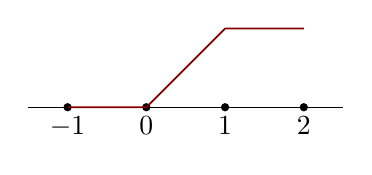
\begin{tikzpicture}
    \draw (-1.5, 0) -- (2.5, 0);
    \foreach \x in {-1,0,1,2} {
      \node [circ] at (\x, 0) {};
      \node [below] at (\x, 0) {$\x$};
    }
    \draw [mred, semithick] (-1, 0) -- (0, 0) -- (1, 1) -- (2, 1);
  \end{tikzpicture}
\end{center}
We can define this function $f$ (in $[0, 1]$) by
\[
  f(x) = x = \inf\left\{\frac{a}{2^n}: a, n \in \N, 0 \leq a \leq 2^n, x \leq \frac{a}{2^n}\right\}.
\]
This is obviously a rather silly way to write our function out. However, this is what we will end up doing in the proof below. So keep this in mind for now.

\begin{proof}
  In this proof, all subsets labeled $C$ are closed, and all subsets labeled $U$ are open.

  First note that normality is equivalent to the following: suppose $C \subseteq U \subseteq X$, where $C$ is open and $U$ is closed. Then there is some $\tilde{C}$ closed, $\tilde{U}$ open such that $C\subseteq \tilde{U} \subseteq \tilde{C} \subseteq U$.

  We start by defining $U_1 = X \setminus C_1$. Since $C_0$ and $C_1$ are disjoint, we know that $C_0 \subseteq U_1$. By normality, there exists $C_{\frac{1}{2}}$ and $U_{\frac{1}{2}}$ such that
  \[
    C_0 \subseteq U_{\frac{1}{2}} \subseteq C_{\frac{1}{2}} \subseteq U_1.
  \]
  Then we can find $C_{\frac{1}{4}}, C_{\frac{3}{4}}, U_{\frac{1}{4}}, U_{\frac{3}{4}}$ such that
  \[
    C_0 \subseteq U_{\frac{1}{4}}\subseteq C_{\frac{1}{4}} \subseteq U_{\frac{1}{2}} \subseteq C_{\frac{1}{2}} \subseteq U_{\frac{3}{4}} \subseteq C_{\frac{3}{4}} \subseteq U_1.
  \]
  Iterating this, we get that for all dyadic rationals $q = \frac{a}{2^n}$, $a, n\in \N, 0 < a < 2^n$, there are some $U_q$ open, $C_q$ closed such that $U_q \subseteq C_q$, with $C_q \subseteq U_{q'}$ if $q < q'$.

  We now define $f$ by
  \[
    f(x) = \inf\left\{q \in (0, 1] \text{ dyadic rational}: x \in U_q\right\},
  \]
  with the understanding that $\inf \emptyset = 1$. We now check the properties desired.
  \begin{itemize}
    \item By definition, we have $0 \leq f(x) \leq 1$.
    \item If $x \in C_0$, then $x \in U_q$ for all $q$. So $f(x) = 0$.
    \item If $x \in C_1$, then $x \not\in U_q$ for all $q$. So $f(x) = 1$.
    \item To show $f$ is continuous, it suffices to check that $\{x: f(x) > \alpha\}$ and $\{x: f(x) < \alpha\}$ for all $\alpha \in \R$, as this shows that the pre-images of all open intervals in $\R$ are open. We know that
      \begin{align*}
        f(x) < \alpha &\Leftrightarrow \inf\{q \in (0, 1)\text{ dyadic rational}: x \in U_q\} < \alpha \\
        &\Leftrightarrow (\exists q)\; q < \alpha \text{ and }x \in U_q\\
        &\Leftrightarrow x \in \bigcup_{q < \alpha} U_q.
      \end{align*}
      Hence we have
      \[
        \{x: f(x) < \alpha\} = \bigcup_{q < \alpha} U_q.
      \]
      which is open, since each $U_q$ is open for all $q$. Similarly we know that
      \begin{align*}
        f(x) > \alpha &\Leftrightarrow \inf\{q: x \in U_q\} > \alpha\\
        &\Leftrightarrow (\exists q > \alpha)\; x \not\in C_q\\
        & x \in \bigcup_{q > \alpha} X \setminus C_q.
      \end{align*}
      Since this is a union of complement of closed sets, this is open.
  \end{itemize}
\end{proof}
With this, we can already say that there are many continuous functions. We can just pick some values on some $C_0, C_1$, and then get a continuous function out of it. However, we can make a stronger statement.

\begin{thm}[Tietze-Urysohn extension theorem]
  Let $X$ be a normal topological space, and $C\subseteq X$ be a closed subset. Suppose $f: C \to \R$ is a continuous function. Then there exists an extension $\tilde{f}: X \to \R$ which is continuous and satisfies $\tilde{f}|_C = f$ and $\|\tilde{f}\|_{C(X)} \leq \|f\|_{C(C)}$.
\end{thm}
This is in some sense similar to the Hahn-Banach theorem, which states that we can extend linear maps to larger spaces.

Note that this implies the Urysohn's lemma, since if $C_0$ and $C_1$ are closed, then $C_0\cup C_1$ is closed.

\begin{proof}
  The idea is to repeatedly use Urysohn's lemma to get better and better approximations. We can assume wlog that $0\leq f(x) \leq 1$ for all $x \in C$. Otherwise, we just translate and rescale our function. Moreover, we can assume that the $\sup\limits_{x \in C} f(x) = 1$. It suffices to find $\tilde{f}: X \to \R$ with $\tilde{f}|_C = f$ with $0 \leq \tilde{f}(x) \leq 1$ for all $x \in X$.

  We define the sequences of continuous functions $f_i: C \to \R$ and $g_i: X \to \R$ for $i \in \N$. We want to think of the sum $\sum_{i = 0}^n g_i$ to be the approximations, and $f_{n + 1}$ the error on $C$.

  Let $f_0 = f$. This is the error we have when we approximate with the zero function.

  We first define $g_0$ on a subset of $X$ by
  \[
    g_0(x) =
    \begin{cases}
      0 & x \in f_0^{-1}\left(\left[0, \frac{1}{3}\right]\right)\\
      \frac{1}{3} & x \in f_0^{-1}\left(\left[\frac{2}{3}, 1\right]\right)
    \end{cases}.
  \]
  We can then extend this to the whole of $X$ with $0 \leq g_0(x) \leq \frac{1}{3}$ for all $x$ by Urysohn's lemma.
  \begin{center}
    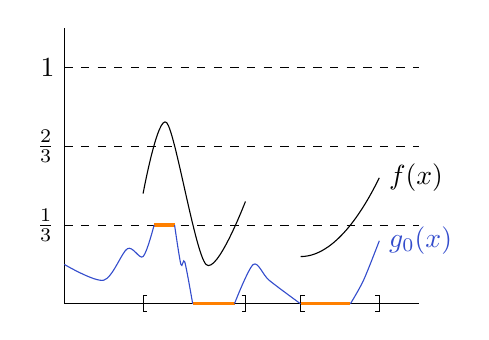
\begin{tikzpicture}
      \draw (0, 0) -- (4.5, 0);
      \draw (0, 0) -- (0, 3.5);
      \node at (0, 1) [left] {$\frac{1}{3}$};
      \node at (0, 2) [left] {$\frac{2}{3}$};
      \node at (0, 3) [left] {$1$};
      \foreach \y in {1, 2, 3} {
        \draw [dashed] (0, \y) -- (4.5, \y);
      }

      \draw plot [smooth] coordinates {(1, 1.4) (1.3, 2.3) (1.8, 0.5) (2.3, 1.3)};
      \draw (3, 0.6) parabola (4, 1.6);

      \draw [very thick, morange] (1.14, 1) -- (1.4, 1);
      \draw [very thick, morange] (1.63, 0) -- (2.17,0);
      \draw [very thick, morange] (3, 0) -- (3.6325, 0);

      \draw (1.05, 0.1) -- +(-0.05, 0) -- +(-0.05, -0.2) -- +(0, -0.2);
      \draw (2.25, 0.1) -- +(0.05, 0) -- +(0.05, -0.2) -- +(0, -0.2);

      \draw (3.05, 0.1) -- +(-0.05, 0) -- +(-0.05, -0.2) -- +(0, -0.2);
      \draw (3.95, 0.1) -- +(0.05, 0) -- +(0.05, -0.2) -- +(0, -0.2);

      \draw [mblue] plot [smooth] coordinates {(0, 0.5) (0.5, 0.3) (0.8, 0.7) (1, 0.6) (1.14, 1)};
      \draw [mblue] plot [smooth] coordinates {(1.4, 1) (1.48, 0.5) (1.53, 0.53) (1.63, 0)};

      \draw [mblue] plot [smooth] coordinates {(2.16, 0) (2.4, 0.5) (2.6, 0.3) (3, 0)};
      \draw [mblue] plot [smooth] coordinates {(3.6325, 0) (3.8, 0.3) (4, 0.8)};
      \node [mblue] at (4, 0.8) [right] {$g_0(x)$};
      \node at (4, 1.6) [right] {$f(x)$};
    \end{tikzpicture}
  \end{center}
  We define
  \[
    f_1 = f_0 - g_0|_C.
  \]
  By construction, we know that $0 \leq f_1 \leq \frac{2}{3}$. This is our first approximation. Note that we have now lowered our maximum error from $1$ to $\frac{2}{3}$. We now repeat this.

  Given $f_i: C \to \R$ with $0 \leq f_i \leq \left(\frac{2}{3}\right)^i$, we define $g_i$ by requiring
  \[
    g_i(x) =
    \begin{cases}
      0 & x \in f_i^{-1}\left(\left[0, \frac{1}{3}\left(\frac{2}{3}\right)^i\right]\right)\\
      \frac{1}{3}\left(\frac{2}{3}\right)^i & x \in f_i^{-1}\left(\left[\left(\frac{2}{3}\right)^{i + 1}, \left(\frac{2}{3}\right)^i\right]\right)\\
    \end{cases},
  \]
  and then extending to the whole of $X$ with $0 \leq g_i \leq \frac{1}{3}\left(\frac{2}{3}\right)^i$ and $g_i$ continuous. Again, this exists by Urysohn's lemma. We then define $f_{i + 1} = f_i - g_i|_C$.

  We then have
  \[
    \sum_{i = 0}^n g_i = (f_0 - f_1) + (f_1 - f_2) + \cdots + (f_n - f_{n + 1}) = f - f_{n + 1}.
  \]
  We also know that
  \[
    0 \leq f_{i + 1} \leq \left(\frac{2}{3}\right)^{i + 1}.
  \]
  We conclude by letting
  \[
    \tilde{f} = \sum_{i = 0}^\infty g_i.
  \]
  This exists because we have the bounds
  \[
    0 \leq g_i \leq \frac{1}{3}\left(\frac{2}{3}\right)^i,
  \]
  and hence $\sum_{i = 0}^n g_i$ is Cauchy. So the limit exists and is continuous by the completeness of $C(X)$.

  Now we check that
  \[
    \sum_{i = 0}^n g_i|_C - f = -f_{n + 1}.
  \]
  Since we know that $\|f_{n + 1}\|_{_C(C)} \to 0$. Therefore, we know that
  \[
    \left.\sum_{i = 0}^\infty g_i\right|_C = \tilde{f}|_C = f.
  \]
  Finally, we check the bounds. We need to show that $0 \leq \tilde{f}(x) \leq 1$. This is true since $g_i \geq 0$ for all $i$, and also
  \[
    |\tilde{f}(x)| \leq \sum_{i = 0}^\infty g_i(x) \leq \sum_{i = 0}^n \frac{1}{3}\left(\frac{2}{3}\right)^i = 1.
  \]
  So done.
\end{proof}
We can already show what was stated last time --- if $K$ is compact Hausdorff, $\{p_1, \cdots, p_n\}\subseteq K$ a finite set of points, and $\{y_1, \cdots, y_n\} \subseteq \R$, then there exists $f: K \to \R$ continuous such that $f(p_i) = y_i$. This is since compact Hausdorff spaces are normal, and singleton points are closed sets in Hausdorff spaces. In fact, we can prove this directly with the Urysohn's lemma, by, say, requesting functions $f_i$ such that $f_i(p_i) = y_i$, $f_i(p_j) = 0$ for $i \not= j$. Then we just sum all $f_i$.

Note that normality is necessary for Urysohn's lemma. Since the Urysohn's lemma is a special case of the Tietze-Urysohn extension theorem, normality is also necessary for the Tietze-Urysohn extension theorem. In fact, the lemma is \emph{equivalent} to normality. Let $C_0, C_1$ be disjoint closed sets of $X$. If there is some $f: X \to \R$ such that $f|_{C_0} = 0$, $f|_{C_1} = 1$, then $U_0 = f^{-1}\left(\left(-\infty, \frac{1}{3}\right)\right)$ and $U_1 = f^{-1}\left(\left(\frac{2}{3}, \infty\right)\right)$ are open disjoint sets such that $C_0 \subseteq U_0, C_1 \subseteq U_1$.

Closedness of $C_0$ and $C_1$ is also necessary in Urysohn's lemma. For example, we cannot extend $f: [0, \frac{1}{2}) \cup (\frac{1}{2}, 1]$ to $[0, 1]$ continuously, where $f$ is defined as
\[
  f(x) =
  \begin{cases}
    0 & x < \frac{1}{2}\\
    1 & x > \frac{1}{2}
  \end{cases}.
\]
\subsection{Arzel\`a-Ascoli theorem}
Let $K$ be compact Hausdorff, and $\{f_n\}_{n = 1}^\infty$ be a sequence of continuous functions $f_n: K \to \R$ (or $\C$). When does $(f_n)$ have a convergent subsequence in $C(K)$? In other words, when is there a subsequence which converges uniformly?

This will be answered by the Arzel\`a-Ascoli theorem. Before we get to that, we look at some examples.
\begin{eg}
  Let $K = [0, 1]$, and $f_n(x) = n$. This does not have a convergent subsequence in $C(K)$ since it does not even have a subsequence that converges pointwise. This is since $f_n$ is unbounded.
\end{eg}
We see that unboundedness is one ``enemy'' that prevents us from having a convergent subsequence.

\begin{eg}
  We again let $K[0, 1])$, and let $f$ be defined as follows:
  \begin{center}
    \begin{tikzpicture}
      \draw [->] (-0.5, 0) -- (3, 0);
      \draw [->] (0, -0.5) -- (0, 2);
      \draw [mred, semithick] (0, 1.5) node [black, left] {$1$} -- (0.6, 0) node [black, below] {$\frac{1}{n}$} -- (2.5, 0) node [black, below] {$1$};
    \end{tikzpicture}
  \end{center}
  We know that $f_n$ does not have a convergent subsequence in $C(K)$, since any subsequence must converge pointwise to
  \[
    f(x) =
    \begin{cases}
      0 & x \not= 0\\
      1 & x = 0
    \end{cases},
  \]
  which is not continuous.
\end{eg}
What is happening here? For every $n$, fixed $x$ every $\varepsilon$, by continuity of $f_n$, there ie some $\delta$ such that $|x - y| < \delta$ implies $|f_n(x) - f_n(y)| < \varepsilon$, but this choice of $\delta$ depends on $n$, and there is no universal choice that works for us. This is another problem that leads to the lack of a limit.

The Arzel\`a-Ascoli theorem tells us these are the only two ``enemies'' that prevent us from extracting a convergent subsequence.

To state this theorem, we first need a definition.
\begin{defi}[Equicontinuous]
  Let $K$ be a topological space, and $F\subseteq C(K)$. We say $F$ is \emph{equicontinuous at $x \in K$} if for every $\varepsilon$, there is some $U$ which is an open neighbourhood of such that
  \[
    (\forall f \in F)(\forall y \in U)\; |f(y) - f(x)| < \varepsilon.
  \]
  We say $F$ is \emph{equicontinuous} if it is equicontinuous at $x$ for all $x \in K$.
\end{defi}

\begin{thm}[Arzel\`a-Ascoli theorem]
  Let $K$ be a compact topological space. Then $F\subseteq C(K)$ is pre-compact, ie. $\bar{F}$ is compact, if and only if $F$ is bounded and equicontinuous.
\end{thm}
This indeed applies to the problem of extracting a uniformly convergent subsequence, since $C(K)$ is a metric space, and compactness is equivalent to sequential compactness. Indeed, let $(f_n)$ be a bounded and equicontinuous sequence in $C(K)$. Then $F = \{f_n: n \in \N\} \subseteq C(K)$ is bounded and equicontinuous. So it is pre-compact, and hence $(f_n)$, being a sequence in $\bar{F}$, has a convergent subsequence.

To prove this, it helps to introduce some more terminology and a few lemmas first.

\begin{defi}[$\varepsilon$-net]
  Let $X$ be a metric space, and let $E\subseteq X$. For $\varepsilon > 0$, we say that $N \subseteq N$ is an \emph{$\varepsilon$-net} for $E$ if and only if $\bigcup_{x \in \N}B(x, \varepsilon) \supseteq E$.
\end{defi}

\begin{defi}[Totally bounded subset]
  Let $X$ be a metric space, and $E\subseteq X$. We say that $E$ is \emph{totally bounded} for every $\varepsilon$, there is a finite $\varepsilon$-net $N_\varepsilon$ for $E$.
\end{defi}

An important result about totally bounded subsets is the following:
\begin{prop}
  Let $X$ be a complete metric space. Then $E\subseteq X$ is totally bounded if and only if for every sequence $\{y_i\}_{i = 1}^\infty \subseteq E$, there is a subsequence which is Cauchy.
\end{prop}

By completeness, we can rewrite this as
\begin{cor}
  Let $X$ be a complete metric space. Then $E\subseteq X$ is totally bounded if and only if $\bar{E}$ is compact.
\end{cor}

We'll prove these later. For now, we assume this corollary and we will prove Arzel\`a-Ascoli theorem.
\begin{thm}[Arzel\`a-Ascoli theorem]
  Let $K$ be a compact topological space. Then $F\subseteq C(K)$ is pre-compact, ie. $\bar{F}$ is compact, if and only if $F$ is bounded and equicontinuous.
\end{thm}

\begin{proof}
  By the previous corollary, it suffices to prove that $F$ is totally bounded if and only if $F$ is bounded and equicontinuous. We first do the boring direction.

  $(\Rightarrow)$ Suppose $F$ is totally bounded. First notice that $F$ is obviously bounded, since $F$ can be written as the finite union of $\varepsilon$-balls, which must be bounded.

  Now we show $F$ is equicontinuous. Let $\varepsilon > 0$. Since $F$ is totally bounded, there exists a finite $\varepsilon$-net for $F$, ie. there is some $\{f_1, \cdots, f_n\} \subseteq F$ such that for every $f \in F$, there exists an $i\in \{1, \cdots, n\}$ such that $\|f - f_i\|_{C(K)} < \varepsilon$.

  Consider a point $x \in K$. Since $\{f_1, \cdots, f_n\}$ are continuous, for each $i$, there exists a neighbourhood $U_i$ of $x$ such that $|f_i (y) - f_i(x)| < \varepsilon$ for all $y \in U_i$.

  Let
  \[
    U = \bigcap_{i = 1}^n U_i.
  \]
  Since this is a finite intersection, $U$ is open. Then for any $f \in F$, $y \in U$, we have we can find some $i$ such that $\|f - f_i\|_{C(K)} < \varepsilon$. So
  \[
    |f(y) - f(x)| \leq |f(y) - f_i(y)| + |f_i(y) + f_i(x)| + |f_i(x) - f(x)| < 3\varepsilon.
  \]
  So $F$ is equicontinuous at $x$. Since $x$ was arbitrary, $F$ is equicontinuous.

  $(\Leftarrow)$ Suppose $F$ is bounded and equicontinuous. Let $\varepsilon > 0$. By equicontinuity, for every $x \in K$, there is some neighbourhood $U_x$ of $x$ such that $|f(y) - f(x)| < \varepsilon$ for all $y \in U_x, f \in F$. Obviously, we have
  \[
    \bigcup_{x \in K}U_x = K.
  \]
  By the compactness of $K$, there are some $\{x_1, \cdots, x_n\}$ such that
  \[
    \bigcup_{i = 1}^n U_{x_i}\supseteq K.
  \]
  Consider the restriction of functions in $F$ to these points. This can be viewed as a bounded subset of $\ell^n_{\infty}$, the $n$-dimensional normed vector space with the supremum norm. Since this is finite-dimensional, boundedness implies total boundedness (due to, say, the compactness of the closed unit ball). In other words, there is a finite $\varepsilon$-net $\{f_1, \cdots, f_n\}$, for every $f \in F$, there is a $j \in \{1, \cdots, m\}$ such that
  \[
    \max_i |f(x_i) - f_j(x_i)| < \varepsilon.
  \]
  Then for every $f \in F$, pick an $f_j$ such that the above holds. Then
  \begin{align*}
    \|f - f_j\|_{C(K)} &= \sup_y |f(y) - f_j(y)|\\
    \intertext{Since $\{U_{x_i}\}$ covers $K$, we can write this as}
    &= \max_i \sup_{y \in U_{x_i}}|f(y) - f_j(y)|\\
    &\leq \max_i \sup_{y \in U_{x_i}} \big(|f(y) - f(x_i)| + |f(x_i) - f_j(x_i)| + |f_j(x_i) - f_j(y)|\big)\\
    &< \varepsilon + \varepsilon +\varepsilon = 3\varepsilon.
  \end{align*}
  So done.
\end{proof}

Now we return to prove the proposition we just used to prove Arzel\`a-Ascoli.
\begin{prop}
  Let $X$ be a (complete) metric space. Then $E\subseteq X$ is totally bounded if and only if for every sequence $\{y_i\}_{i = 1}^\infty \subseteq E$, there is a subsequence which is Cauchy.
\end{prop}

\begin{proof}
  $(\Rightarrow)$ Let $E \subseteq X$ be totally bounded, $\{y_i\} \in E$. For every $j \in \N$, there exists a finite $\frac{1}{j}$-net, call it $N_j$.

  Now since $N_1$ is finite, there is some $x_1$ such that there are infinitely many $y_i$'s in $B(x_1, 1)$. Pick the first $y_i$ in $B(x_1, 1)$ and call it $y_{i_1}$.

  Now there is some $x_2 \in N_2$ such that there are infinitely many $y_i$'s in $B(x_1, 1) \cap B(x_2, \frac{1}{2})$. Pick the one with smallest value of $i > i_1$, and call this $y_{i_2}$. Continue till infinity.

  This procedure gives a sequence $x_i \in N_i$ and a subsequence $\{y_{i_k}\}$, and also
  \[
    y_{i_n} \in \bigcap_{j = 1}^n B\left(x_j, \frac{1}{j}\right).
  \]
  It is easy to see that $\{y_{i_n}\}$ is Cauchy since if $m > n$, then $d(y_{i_m}, y_{i_n}) < \frac{2}{n}$.

  $(\Leftarrow)$ Suppose $E$ is not totally bounded. So there is no finite $\varepsilon$-net. Pick any $y_1$. Pick $y_2$ such that $d(y_1, y_2) \geq \varepsilon$. This exists because there is no finite $\varepsilon$-net.

  Now given $y_1, \cdots, y_n$ such that $d(y_i, y_j) \geq \varepsilon$ for all $i, j = 1, \cdots, n$, $i \not= j$, we pick $y_{n + 1}$ such that $d(y_{n + 1}, y_j) \geq \varepsilon$ for all $j = 1, \cdots, n$. Again, this exists because there is no finite $\varepsilon$-net. Then clearly any subsequence of $\{y_n\}$ is not Cauchy.
\end{proof}
Note that the first part is similar to the proof of Bolzano-Weierstrass in $\R^n$ by repeated bisection.

Recall that at the beginning of the chapter, we have seen that boundedness and equicontinuity assumptions are necessary. The compactness of $K$ is also important. Let $X = \R$, which is not compact, and let $\phi \in C_c^{\infty}$, an infinitely differentiable function with compact support, say, the bump function.
\begin{center}
  \begin{tikzpicture}[scale=1.5]
    \draw [->] (-2, 0) -- (2, 0) node [right] {$x$};
    \draw [->] (0, -0.5) -- (0, 1);

    \draw [semithick, domain=-0.999:0.999, mblue] plot (\x, {exp (-1 / (1 - \x * \x))});
    \draw [semithick, mblue] (-1.5, 0) -- (-1, 0);
    \draw [semithick, mblue] (1, 0) -- (1.5, 0);
  \end{tikzpicture}
\end{center}
We now let $f_n(x) = \phi(x - n)$, ie. we shift our bump function to the right by $n$ units. This sequence is clearly bounded and equicontinuous, but this has no convergent subsequence --- $f_n$ converges pointwise to the zero function, but the convergence is not uniform, and this is true for arbitrary subsequences as well.

We are going to look at some applications of the theorem:

\begin{eg}
  Let $K\subseteq \R$ be a compact space, $\{f_n\}_{n = 1}^\infty$ be a sequence of continuously differentiable functions in $C(K)$, such that
  \[
    \sup_x \sup_n (|f_n(x)| + |f_n'(x)|) < C
  \]
  for some $C$. Then there is a convergent subsequence. We clearly have uniform boundedness. To obtain equicontinuity, since the derivative is bounded, by the mean value theorem, we have
  \[
    \frac{|f_n(x) - f_n(y)|}{|x - y|} = |f_n'(z)| \leq C
  \]
  So
  \[
    |f_n(x) - f_n(y)| \leq C |x - y|.
  \]
\end{eg}

Consider the ordinary differential equation $x' = f(x)$ with the boundary conditions $x(0) = x_0 \in \R^n$. Recall from IB Analysis II that Picard-Lindelof theorem says that if $f$ is a Lipschitz function, then there exists some $\varepsilon > 0$ such that the ODE has a \emph{unique} solution in $(-\varepsilon, \varepsilon)$.

What if $f$ is not Lipschitz? If so, we can get the following
\begin{thm}[Peano*]
  Given $f$ continuous, then there is some $\varepsilon > 0$ such that $x' = f(x)$ with boundary condition $x(0) = x_0 \in \R$ has a solution in $(-\varepsilon, \varepsilon)$.
\end{thm}
Note that uniqueness is false. For example, if $x' = \sqrt{|x|}$, $x(0) = 0$, then $x(t) = 0$ and $x(t) = t^2$ are both solutions.

\begin{proof}(sketch)
  We approximate $f$ by a sequence of continuously differentiable functions $f_n$ such that $\|f - f_n\|_{C(K)} \to 0$ for some $K\subseteq \R$. We use Picard-Lindelof to get a solution for all $n$. Then we use the ode to get estimates for the solution. Finally, we can use Arzel\`a-Ascoli to extract a limit as $n \to \infty$. We can then show it is indeed a solution.
\end{proof}

\subsection{Stone-Weierstrass theorem}
Here we will prove the Stone-Weierstrass theorem, which is a generalization of the classical Weierstrass approximation theorem.
\begin{thm}[Weierstrass approximation theorem]
  The set of polynomials are dense in $C([0, 1])$.
\end{thm}
This tells us that $C([0, 1])$ is not too ``big'' because it is has a dense subset of ``nice'' functions.

We will try to generalize this for more general domains. Note that for this section, real-valued and complex-valued continuous functions are somewhat differentiable. So we will write these as $C_{\R}(K)$ and $C_{\C}(K)$.

To state this theorem, we need some definitions.

\begin{defi}[Algebra]
  A vector space $(V, +)$ is called an \emph{algebra} if there is an operation (called multiplication) $\ph: V \to V$ such that $(V, +, \ph)$ is a \emph{rng} (ie. ring not necessarily with multiplicative identity). Also, $\lambda(\mathbf{v}\cdot \mathbf{w}) = (\lambda \mathbf{v})\cdot \mathbf{w} = \mathbf{v}\cdot (\lambda \mathbf{w})$ for all $\lambda \in \F$, $\mathbf{v}, \mathbf{w} \in \F$.

  If $V$ is in addition a normed vector space and
  \[
    \|\mathbf{v}\cdot \mathbf{w}\|_V \leq \|\mathbf{v}\|_V \cdot \|\mathbf{w}\|_V
  \]
  for all $\mathbf{v}, \mathbf{w} \in V$, then we say $V$ is a \emph{normed algebra}.

  If $V$ complete normed algebra, we say $V$ is a \emph{Banach algebra}.

  If $V$ is an algebra that is commutative as a rng, then we say $V$ is a \emph{commutative algebra}.

  If $V$ is an algebra with multiplicative identity, then $V$ is a \emph{unital algebra}.
\end{defi}

\begin{eg}
  $C(K)$ is a commutative, unital, Banach algebra.
\end{eg}

\begin{eg}
  Recall from the example sheets that if $T_1, T_2: V\to V$, then
  \[
    \|T_1 \circ T_2\|_{\mathcal{B}(V, V)} \leq \|T_1\|_{\mathcal{B}(V, V)}\|T_2\|_{\mathcal{B}(V, V)}.
  \]
  So $\mathcal{B}(V, V)$ is a unital normed algebra.
\end{eg}

We will need this language to generalize the Weierstrass approximation theorem. The main problem in doing so is that we have to figure out what we can generalize polynomials to. This is why we need these funny definitions.

\begin{thm}[Stone-Weierstrass theorem]
  Let $K$ be compact, and $\mathcal{A} \subseteq C_{\R}(K)$ be a subalgebra (ie. it is a subset that is closed under the operations) with the property that it separates points, ie. for every $x, y \in K$ distinct, there exists some $f \in \mathcal{A}$ such that $f(x) \not= f(y)$. Then either $\bar{\mathcal{A}} = C_\R(K)$ or there is some $x_0 \in K$ such that
  \[
    \bar{\mathcal{A}} = \{f \in C_{\R(K)}: f(x_0) = 0\}.
  \]
\end{thm}
Note that it is not possible that $\bar{A}$ is always zero on $2$ or more points, since $\mathcal{A}$ separates points.

This indeed implies the Weierstrass approximation theorem, since polynomials separates points (consider the polynomial $x$), and the polynomial $1$ is never $0$ for all $x$. In fact, this works also for polynomials on compact subsets of $\R^n$.

Note, however, that the second case of Stone-Weierstrass theorem can actually happen. For example, consider $K = [0, 1]$ compact, and $\mathcal{A}$ be the algebra generated by $x$. Then $\bar{A} = \{f \in C_\R(K): f(0) = 0\}$.

We will prove this in using two lemmas:
\begin{lemma}
  Let $K$ compact, $\mathcal{L} \subseteq C_\R(K)$ be a subset which is closed under taking maximum and minimum, ie. if $f, g \in \mathcal{L}$, then $\max\{f, g\} \in \mathcal{L}$ and $\min \{f, g\} \in \mathcal{L}$ (with $\max\{f, g\}$ defined as $\max\{f, g\}(x) = \max\{f(x), g(x)\}$, and similarly for minimum).

  Then given $g \in C_\R(K)$, suppose for any $\varepsilon > 0$ and $x, y \in K$, there exists $f_{x, y} \in \mathcal{L}$ such that
  \[
    |f_{x, y}(x) - g(x)| < \varepsilon,\quad |f_{x, y}(y) - g(y)| < \varepsilon.
  \]
  Then there exists some $f \in \mathcal{L}$ such that
  \[
    \|f - g\|_{C_\R(K)} < \varepsilon,
  \]
  ie. $g \in \bar{\mathcal{L}}$.
\end{lemma}
This means that if we are allowed to take maximums and minimums, to be able to approximate a function, we just need to be able to approximate it at any two points.

The idea is to next show that if $\mathcal{A}$ is a subalgebra, then $\bar{\mathcal{A}}$ is closed under taking maximum and minimum. Then use the ability to separate points to find $f_{x, y}$, and prove that we can approximate arbitrary functions.

\begin{proof}
  Let $g \in C_\R(K)$ and $\varepsilon > 0$ be given. So for every $x, y \in K$, there is some $f_{x, y} \in \mathcal{L}$ such that
  \[
    |f_{x, y}(x) - g(x)| < \varepsilon,\quad |f_{x, y}(y) - g(y)| < \varepsilon.
  \]
  Since $f_{x, y}$ is continuous, there is some $U_{x, y}$ containing $y$ open such that
  \[
    |f_{x, y}(z) - g(z)| < \varepsilon
  \]
  for all $z \in U_{x, y}$. Since
  \[
    \bigcup_{y \in K} U_{x, y} \supseteq K,
  \]
  by compactness of $K$, there exists a some $\mathbf{y}_1, \cdots, \mathbf{y}_n$ such that
  \[
    \bigcup_{i = 1}^n U_{x, y_i}\supseteq K.
  \]
  Now let
  \[
    f_x(z) = \min\{f_{x, y_1}(z), \cdots, f_{x, y_n}(z)\}
  \]
  for every $z \in K$. By assumption, $f_x \in \mathcal{L}$. Now let $z \in K$ be arbitrary. Suppose $z \in U_{x y_i}$. Then
  \[
    f_{x, y_i}(z) < g(z) + \varepsilon.
  \]
  Hence, since $f_x$ is the minimum, for any $z$, we have
  \[
    f_x(z) < g(z) + \varepsilon.
  \]
  On the other hand, we still have $|f_x(x) - g(x)| < \varepsilon$. We are going to play the same game with this. By continuity of $f_x$, there is $V_x$ containing $x$ open such that
  \[
    |f_x(w) - g(w)| < \varepsilon
  \]
  for all $w \in V_x$. Since
  \[
    \bigcup_{x\in K} V_x \supseteq K,
  \]
  by compactness of $K$, there is some $\{x_1, \cdots, x_m\}$ such that
  \[
    \bigcup_{j = 1}^m V_{x_j} \supseteq K.
  \]
  Define
  \[
    f(z) = \max\{f_{x_1}(z), \cdots, f_{x_m}(z)\}.
  \]
  Again, by assumption, $f \in \mathcal{L}$. We still have our first bound
  \[
    f(z) < g(z) + \varepsilon.
  \]
  Moreover, by the same argument as above, we also have the bound
  \[
    f(z) > g(z) - \varepsilon.
  \]
  Therefore we have
  \[
    \|f - g\|_{C_\R (K)} < \varepsilon.
  \]
\end{proof}

\begin{lemma}
  Let $\mathcal{A}\subseteq C_\R(K)$ be a subalgebra that is a closed subset in the topology of $C_\R(K)$. Then $\mathcal{A}$ is closed under taking maximum and minimum.
\end{lemma}

\begin{proof}
  First note that
  \begin{align*}
    \max\{f(x), g(x)\} &= \frac{1}{2}(f(x) + g(x)) + \frac{1}{2}|f(x) - g(x)|,\\
    \min\{f(x), g(x)\} &= \frac{1}{2}(f(x) + g(x)) - \frac{1}{2}|f(x) - g(x)|.
  \end{align*}
  Since $\mathcal{A}$ is an algebra, it suffices to show that $f \in A$ implies $|f| \in A$ for every $f$ such that $\|f\|_{C\R(K)} \leq 1$.

  The key observation is the following: consider the function $h(x) = \sqrt{x + \varepsilon^2}$. Then $h(x^2)$ approximates $|x|$. This has the property that the Taylor expansion of $h(x)$ centered at $x = \frac{1}{2}$ is uniformly convergent for $x \in [0, 1]$. Therefore there exists a polynomial $S(x)$ such that
  \[
    |S(x) - \sqrt{x + \varepsilon^2}| < \varepsilon.
  \]
  Now note that $S(x) - S(0)$ is a polynomial with no constant term. Therefore, since $\mathcal{A}$ is an algebra, if $f \in \mathcal{A}$, then $S(f^2) - S(0) \in \mathcal{A}$ by closure.

  Now look at
  \[
    \||f| - (S(f^2) - S(0))\|_{C_\R(K)} \leq \||f| - \sqrt{f^2 + \varepsilon^2}\| + \|\sqrt{f^2 - \varepsilon^2} - S(f^2)\| + \|S(0)\|
  \]
  We will make each individual term small. For the first term, note that
  \[
    \sup_{x \in [0, 1]} |x - \sqrt{x^2 + \varepsilon^2}| = \sup_{x \in [0, 1]} \frac{\varepsilon^2}{|x + \sqrt{x^2 + \varepsilon^2}|} = \varepsilon.
  \]
  So the first term is at most $\varepsilon$. The second term is also easy, since $S$ is chosen such that $|S(x) - \sqrt{x + \varepsilon^2}| < \varepsilon$, and $f(x) < \varepsilon$ for all $x$. So it is again bounded by $\varepsilon$.

  By the same formula, $|S(0) - \sqrt{0 + \varepsilon^2}| < \varepsilon$. So $|S(0)| < 2\varepsilon$. So
  \[
    \||f| - (S(f^2) - S(0))\|_{C_\R(K)} < 4\varepsilon.
  \]
  Since $\varepsilon > 0$ and $\mathcal{A}$ is closed in the topology of $C_{\R}(K)$, $f\in \mathcal{A}$ and $\|f\|_{C_\R(K)} \leq 1$ implies that $|f| \in \mathcal{A}$.
\end{proof}

We will now combine both lemmas and prove the Stone-Weierstrass lemma.
\begin{thm}[Stone-Weierstrass theorem]
  Let $K$ be compact, and $\mathcal{A} \subseteq C_{\R}(K)$ be a subalgebra (ie. it is a subset that is closed under the operations) with the property that it separates points, ie. for every $x, y \in K$ distinct, there exists some $f \in \mathcal{A}$ such that $f(x) \not= f(y)$. Then either $\bar{\mathcal{A}} = C_\R(K)$ or there is some $x_0 \in K$ such that
  \[
    \bar{\mathcal{A}} = \{f \in C_{\R(K)}: f(x_0) = 0\}.
  \]
\end{thm}

\begin{proof}
  Note that there are two possible outcomes. We will first look at the first possibility.

  Consider the case where for all $x \in K$, there is some $f \in \mathcal{A}$ such that $f(x) \not= 0$. Let $g \in C_{\R}(K)$ be given. By our previous lemmas, to approximate $g$ in $\bar{\mathcal{A}}$, we just need to show that we can approximate $g$ at two points. So given any $\varepsilon > 0$, $x, y \in K$, we want to find $f_{x, y} \in \mathcal{A}$ such that
  \[
    |f_{x, y}(x) - g(x)| < \varepsilon,\quad |f_{x, y}(y) - g(y)| < \varepsilon. \tag{$*$}
  \]
  For every $x, y \in K$, $x \not= y$, we first show that there exists $h_{x, y} \in \mathcal{A}$ such that $h_{x, y}(x) \not= 0$, and $h_{x, y}(x) \not= h_{x, y}(y)$. This is easy to see. By our assumptions, we can find the following functions:
  \begin{enumerate}
    \item There exists $h_{x, y}^{(1)}$ such that $h_{x, y}^{(1)} \not= h_{x, y}^{(1)}(y)$
    \item There exists $h_{x, y}^{(2)}$ such that $h_{x, y}^{(2)}(x) \not= 0$.
    \item There exists $h_{x, y}^{(3)}$ such that $h_{x, y}^{(3)}(y) \not= 0$.
  \end{enumerate}
  Then it is an easy exercise to show that some linear combination of $h_{x, y}^{(1)}$ and $h_{x, y}^{(2)}$ and $h_{x, y}^{(3)}$ works, say $h_{x, y}$.

  We will want to find our $f_{x, y}$ that satisfies $(*)$. But we will do better. We will make it equal $g$ on $x$ and $y$. The idea is to take linear combinations of $h_{x, y}$ and $h_{x, y}^2$. Instead of doing the messy algebra to show that we can find a working linear combination, just notice that $(h_{x, y}(x), h_{x, y}(y))$ and $(h_{x, y}(x)^2, h_{x, y}(y)^2)$ are linearly independent vectors in $\R^2$. Therefore there exists $\alpha, \beta \in \R$ such that
  \[
    \alpha(h_{x, y}(x), h_{x, y}(y)) + \beta(h_{x, y}(x)^2, h_{x, y}(y)^2) = (g(x), g(y)).
  \]
  So done.

  In other case, given $\mathcal{A}$, suppose there is $x_0 \in K$ such that $f(x_0) = 0$ for all $f \in \mathcal{A}$. Consider the algebra
  \[
    \mathcal{A}' = \mathcal{A} + \lambda 1 = \{f + \lambda 1: f \in \mathcal{A}, \lambda \in \R\}
  \]
  Since $\mathcal{A}$ separates points, and for any $\mathbf{x} \in K$, there is some $f \in \mathcal{A}'$ such that $f(x) \not= 0$ (eg. $f = 1$), by the previous part, we know that $\bar{\mathcal{A}}' = C_{\R}(K)$.

  Now note that
  \[
    \bar{\mathcal{A}} \subseteq \{f \in C_\R(K): f(x_0) = 0\} = B.
  \]
  So we suffices to show that we have equality, ie. for any $g \in B$ and $\varepsilon > 0$, there is some $f \in \mathcal{A}$ such that
  \[
    \|f - g\|_{C_\R(K)} < \varepsilon.
  \]
  Since $\bar{\mathcal{A}}' = C_\R(K)$, given such $g$ and $\varepsilon$, there is some $f \in \mathcal{A}$ and $\lambda_0 \in \R$ such that
  \[
    \|g - (f + \lambda 1)\|_{C_{\R}(K)} < \varepsilon.
  \]
  But $g(x_0) = f(x_0) = 0$, which implies that $|\lambda| < \varepsilon$. Therefore $\|g - f\|_{C_\R(K)} < 2 \varepsilon$. So done.
\end{proof}

What happens for $C_\C(K)$?
\begin{eg}
  Let $K = \overline{B(0, 1)} \subseteq \C$, and let $\mathcal{A}$ be the set of polynomials on $\overline{B(0, 1)}$. We will show that $\bar{\mathcal{A}} \not= C_{\C}(\overline{B(0, 1)})$.

  Consider $f(z) = \bar{z}$. This is not in the closure of $\mathcal{A}$, since this is not holomorphic, but the uniform limit of any sequence of holomorphic is holomorphic (by Morera's theorem, ie. $f$ is holomorphic iff $\oint_\gamma f(z) \;\d z = 0$ for all closed piecewise smooth curve $\gamma$).
\end{eg}
Hence we need an additional condition on this. It turns out that this rather simple example is the only way in which things can break. We have the following:

\begin{thm}[Complex version of Stone-Weierstrass theorem]
  Let $K$ be compact and $\mathcal{A} \subseteq C_\C(K)$ be a subalgebra over $\C$ which separates points and is closed under complex conjugation (ie. if $f \in \mathcal{A}$, then $\bar{f} = \mathcal{A}$). Then either $\bar{\mathcal{A}} = C_\C(K)$ or these is an $x_0$ such that $\bar{A} = \{f \in C_\C(K): f(x_0) = 0\}$.
\end{thm}

\begin{proof}
  It suffices to show that either $\bar{\mathcal{A}} \supseteq C_{\R}(K)$ or there exists a point $x_0$ such that $\bar{\mathcal{A}} \supseteq \{f \in C_{\R}(K): f(x_0) = 0\}$, since we can always break a complex function up into its real and imaginary parts.

  Now consider
  \[
    \mathcal{A}' = \left\{\frac{f + \bar{f}}{2}: f \in \mathcal{A}\right\} \cup \left\{\frac{f - \bar{f}}{2i}: f \in \mathcal{A}\right\}.
  \]
  Now note that by closure of $\mathcal{A}$, we know that $\mathcal{A}'$ is a subset of $\mathcal{A}$ and is a subalgebra of $C_\R(K)$ over $\R$, which separates points. Hence by the real version of Stone-Weierstrass, either $\bar{\mathcal{A}'} = C_\R(K)$ or there is some $x_0$ such that $\bar{\mathcal{A}'} = \{f \in C_\R(K): f(x_0) = 0\}$. So done.
\end{proof}

\section{Hilbert spaces}
\subsection{Inner product spaces}
We have just looked at continuous functions on some compact space $K$. Another important space is the space of square-integrable functions. Consider the space
\[
  L^2(\R) = \left\{f: f\text{ is Lebesgue integrable} : \int |f|^2 < \infty\right\} / {\sim},
\]
where $f \sim g$ if $f = g$ is Lebesgue almost everywhere.

One thing we like to think about is the Fourier series. Recall that for $f \in C(S^1)$, we have defined, for each $k \in \Z$,
\[
  \hat{f}(k) = \frac{1}{2\pi} \int_{-\pi}^\pi e^{-ikx}f(x)\;\d x,
\]
and we have defined the partial sum
\[
  S_N(f)(x) = \sum_{n = -N}^N e^{inx} \hat{f}(k).
\]
We have previously seen that even if $f$ is continuous, it is possible that the partial sums $S_N$ do not converge, even pointwise. However, we can ask for something weaker:

\begin{prop}
  Let $f \in C(S^1)$. Then
  \[
    \lim_{N \to \infty} \frac{1}{2\pi}\int_{-\pi}^\pi |f(x) - S_N(f)(x)|^2 \;\d x = 0.
  \]
\end{prop}
We will prove this later. However, the key points of the proof is the ``orthogonality'' of $\{e^{inx}\}$. More precisely, we have
\[
  \frac{1}{2\pi} \int_{-\pi}^\pi e^{inx}e^{-imx} \;\d x = 0\text{ if } m\not= n.
\]
The introduction of Hilbert spaces is in particular a way to put this in a general framework. We want to introduce an extra structure that gives rise to ``orthogonality''.

\begin{defi}[Inner product]
  Let $V$ be a vector space over $\R$ or $\C$. We say $p: V \times V \to \R$ or $\C$ is an \emph{inner product} on $V$ it satisfies
  \begin{enumerate}
    \item $p(\mathbf{v}, \mathbf{w}) = \overline{p(\mathbf{w}, \mathbf{v})}$ for all $\mathbf{v}, \mathbf{w} \in V$.\hfill(antisymmetry)
    \item $p(\lambda_1 \mathbf{v}_1 + \lambda_2 \mathbf{v}_2, \mathbf{u}) = \lambda_1 p(\mathbf{v}_1, \mathbf{w}) + \lambda_2 p(\mathbf{v}_2, \mathbf{w})$. \hfill(linearity in first argument)
    \item $p(\mathbf{v}, \mathbf{v}) \geq 0$ for all $\mathbf{v} \in V$ and equality holds iff $\mathbf{v} = \mathbf{0}$.\hfill(non-negativity)
  \end{enumerate}
  We will often denote an inner product by $p(\mathbf{v}, \mathbf{w}) = \bra \mathbf{v}, \mathbf{w}\ket$. We call $(V, \bra\ph ,\ph \ket)$ an inner product space.
\end{defi}

\begin{defi}[Orthogonality]
  In an inner product space, $\mathbf{v}$ and $\mathbf{w}$ are \emph{orthogonal} if $\bra \mathbf{v}, \mathbf{w} \ket = 0$.
\end{defi}

Orthogonality and the inner product is important when dealing with vector spaces. For example, recall that when working with finite-dimensional spaces, we had things like hermitian matrices, orthogonal matrices and normal matrices. All these are in some sense defined in terms of the inner product and orthogonality. More fundamentally, when we have a finite-dimensional vector spaces, we often write the vectors as a set of $n$ coordinates. To define this coordinate system, we start by picking $n$ orthogonal vectors (which are in fact orthonormal), and then the coordinates are just the projections onto these orthogonal vectors.

Hopefully, you are convinced that inner products are important. So let's see what we can get if we put in inner products to arbitrary vector spaces.


We will look at some easy properties of the inner product.
\begin{prop}[Cauchy-Schwarz inequality]
  Let $(V, \bra \ph,\ph\ket)$ be an inner product space. Then for all $\mathbf{v}, \mathbf{w} \in V$,
  \[
    |\bra \mathbf{v}, \mathbf{w}\ket| \leq \sqrt{\bra \mathbf{v}, \mathbf{v}\ket \bra \mathbf{w}, \mathbf{w}\ket},
  \]
  with equality iff there is some $\lambda \in \R$ or $\C$ such that $\mathbf{v} = \lambda \mathbf{w}$ or $\mathbf{w} = \lambda \mathbf{v}$.
\end{prop}

\begin{proof}
  wlog, we can assume $\mathbf{w} \not= 0$. Otherwise, this is trivial. Moreover, assume $\bra \mathbf{v}, \mathbf{w}\ket \in \R$. Otherwise, we can just multiply $\mathbf{w}$ by some $e^{i\alpha}$.

  By non-negativity, we know that for all $t$, we have
  \begin{align*}
    0 &\leq \bra \mathbf{v} + t\mathbf{w}, \mathbf{v} + t\mathbf{w}\ket\\
    &= \bra \mathbf{v}, \mathbf{v}\ket + 2t\bra \mathbf{v}, \mathbf{w}\ket + t^2 \bra \mathbf{w}, \mathbf{w}\ket.
  \end{align*}
  Therefore, the discriminant of this quadratic polynomial in $t$ is non-positive, ie.
  \[
    4(\bra \mathbf{v}, \mathbf{w}\ket)^2 - 4\bra \mathbf{v}, \mathbf{v}\ket \bra \mathbf{w}, \mathbf{w}\ket \leq 0,
  \]
  from which the result follows.

  Finally, note that if equality holds, then the discriminant is $0$. So the quadratic has exactly one root. So there exists $t$ such that $\mathbf{v} + t\mathbf{w} = 0$, which of course implies $\mathbf{v} = -t\mathbf{w}$.
\end{proof}

\begin{prop}
  Let $(V, \bra \ph, \ph\ket)$ be an inner product space. Then
  \[
    \|\mathbf{v}\| = \sqrt{\bra \mathbf{v}, \mathbf{v}\ket}
  \]
  defines a norm.
\end{prop}

\begin{proof}
  The first two axioms of the norm are easy to check, since it follows directly from definition of the inner product that $\|\mathbf{v}\| \geq 0$ with equality iff $\mathbf{v} = \mathbf{0}$, and $\|\lambda \mathbf{v}\| = |\lambda| \|\mathbf{v}\|$.

  The only non-trivial thing to check is the triangle inequality. We have
  \begin{align*}
    \|\mathbf{v} + \mathbf{w}\|^2 &= \bra \mathbf{v} + \mathbf{w}, \mathbf{v} + \mathbf{w}\ket\\
    &= \|\mathbf{v}\|^2 + \|\mathbf{w}\|^2 + |\bra \mathbf{v}, \mathbf{w}\ket| + |\bra \mathbf{w}, \mathbf{v}\ket|\\
    &\leq \|\mathbf{v}\|^2 + \|\mathbf{w}\|^2 + 2\|\mathbf{v}\|\|\mathbf{w}\| \\
    &= (\|\mathbf{v}\| + \|\mathbf{w}\|)^2
  \end{align*}
  Hence we know that $\|\mathbf{v} + \mathbf{w}\| \leq \|\mathbf{v} \| + \|\mathbf{w}\|$.
\end{proof}

This motivates the following definition:
\begin{defi}[Euclidean space]
  A normed vector space $(V, \|\ph\|)$ is a \emph{Euclidean space} if there exists an inner product $\bra \ph,\ph\ket$ such that
  \[
    \|\mathbf{v}\| = \sqrt{\bra \mathbf{v}, \mathbf{v}\ket}.
  \]
\end{defi}

\begin{prop}
  Let $(E, \|\ph\|)$ be a Euclidean space. Then there is a \emph{unique} inner product $\bra \ph,\ph\ket$ such that $\|\mathbf{v}\| = \sqrt{\bra \mathbf{v}, \mathbf{v}\ket}$.
\end{prop}

\begin{proof}
  The real and complex cases are slightly different.

  First suppose $E$ is a vector space over $\R$, and suppose also that we have an inner product $\bra \ph,\ph\ket$ such that $\|\mathbf{v}\| = \sqrt{\bra \mathbf{v}, \mathbf{v}\ket }$. Then
  \[
    \bra \mathbf{v} + \mathbf{w}, \mathbf{v} + \mathbf{w}\ket = \|\mathbf{v}\|^2 + 2\bra \mathbf{v}, \mathbf{w}\ket + \|\mathbf{w}\|^2.
  \]
  So we get
  \[
    \bra \mathbf{v}, \mathbf{w}\ket = \frac{1}{2} (\|\mathbf{v} + \mathbf{w}\|^2 - \|\mathbf{v}\|^2 + \|\mathbf{w}\|^2).\tag{$*$}
  \]
  In particular, the inner product is completely determined by the norm. So this must be unique.

  Now suppose $E$ is a vector space over $\C$. We have
  \begin{align*}
    \bra \mathbf{v} + \mathbf{w}, \mathbf{v} + \mathbf{w}\ket &= \|\mathbf{v}\|^2 + \|\mathbf{w}\|^2 + \bra \mathbf{v}, \mathbf{w}\ket + \bra \mathbf{w}, \mathbf{v}\ket\tag{1}\\
    \bra \mathbf{v} - \mathbf{w}, \mathbf{v} - \mathbf{w}\ket &= \|\mathbf{v}\|^2 + \|\mathbf{w}\|^2 - \bra \mathbf{v}, \mathbf{w}\ket - \bra \mathbf{w}, \mathbf{v}\ket\tag{2}\\
    \bra \mathbf{v} +i\mathbf{w}, \mathbf{v} +i\mathbf{w}\ket &= \|\mathbf{v}\|^2 + \|\mathbf{w}\|^2 -i\bra \mathbf{v}, \mathbf{w}\ket +i\bra \mathbf{w}, \mathbf{v}\ket\tag{3}\\
    \bra \mathbf{v} -i\mathbf{w}, \mathbf{v} -i\mathbf{w}\ket &= \|\mathbf{v}\|^2 + \|\mathbf{w}\|^2 +i\bra \mathbf{v}, \mathbf{w}\ket -i\bra \mathbf{w}, \mathbf{v}\ket\tag{4}
  \end{align*}
  Now consider $(1) + (2) + i(3) - i(4)$. Then we obtain
  \[
    \|\mathbf{v} + \mathbf{w}\|^2 - \|\mathbf{v} - \mathbf{w}\|^2 + i\|\mathbf{v} + i\mathbf{w}\|^2 - i\|\mathbf{v} - i\mathbf{w}\|^2 = 4\bra \mathbf{v}, \mathbf{w}\ket.\tag{$\dagger$}
  \]
  So again $\bra \mathbf{v}, \mathbf{w}\ket$ is again determined by the norm.
\end{proof}
Note that the identities $(*)$ and $(\dagger)$ are sometimes known as the \emph{polarization identities}.

\begin{defi}[Hilbert space]
  A \emph{Euclidean space} $(E, \|\ph\|)$ is a \emph{Hilbert space} if it is complete.
\end{defi}

We will prove certain properties of the inner product.
\begin{prop}[Parallelogram law]
  Let $(E, \|\ph\|)$ be a Euclidean space. Then for $\mathbf{v}, \mathbf{w} \in E$, we have
  \[
    \|\mathbf{v} - \mathbf{w}\|^2 + \|\mathbf{v} + \mathbf{w}\|^2 = 2\|\mathbf{v}\|^2 + 2\|\mathbf{w}\|^2.
  \]
\end{prop}
This is called the parallelogram law because it says that for any parallelogram, the sum of the square of the lengths of the diagonals is the sum of square of the lengths of the two sides.
\begin{center}
  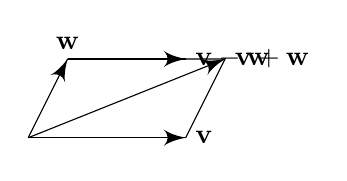
\begin{tikzpicture}
    \draw (2, 0) -- (2.5, 1) -- (0.5, 1);
    \draw [->] (0, 0) -- (2, 0) node [right] {$\mathbf{v}$};
    \draw [->] (0, 0) -- (0.5, 1) node [above] {$\mathbf{w}$};
    \draw [->] (0, 0) -- (2.5, 1) node [right] {$\mathbf{v} + \mathbf{w}$};
    \draw [->] (0.5, 1) -- (2, 1) node [right] {$\mathbf{v} - \mathbf{w}$};
  \end{tikzpicture}
\end{center}

\begin{proof}
  This is just simple algebraic manipulation. We have
  \begin{align*}
    \|\mathbf{v} - \mathbf{w}\|^2 + \|\mathbf{v} + \mathbf{w}\|^2 &= \bra \mathbf{v} - \mathbf{w}, \mathbf{v} - \mathbf{w}\ket + \bra \mathbf{v} + \mathbf{w}, \mathbf{v} + \mathbf{w}\ket\\
    &= \bra \mathbf{v}, \mathbf{v}\ket - \bra \mathbf{v}, \mathbf{w}\ket - \bra \mathbf{w}, \mathbf{v}\ket + \bra \mathbf{w}, \mathbf{w}\ket\\
    &+ \bra \mathbf{v}, \mathbf{v}\ket + \bra \mathbf{v}, \mathbf{w}\ket + \bra \mathbf{w}, \mathbf{v}\ket + \bra \mathbf{w}, \mathbf{w}\ket\\
    &= 2\bra \mathbf{v}, \mathbf{v}\ket + 2 \bra \mathbf{w}, \mathbf{w}\ket.
  \end{align*}
\end{proof}

\begin{prop}
  Let $(E, \|\ph\|)$ be a Euclidean space, and let $\mathbf{v} \mathbf{w}\in E$ be orthogonal. Then
  \[
    \|\mathbf{v} + \mathbf{w}\|^2 = \|\mathbf{v}\|^2 + \|\mathbf{w}\|^2.
  \]
\end{prop}

\begin{proof}
  \begin{align*}
    \|\mathbf{v} + \mathbf{w}\|^2 &= \bra \mathbf{v} + \mathbf{w}, \mathbf{v} - \mathbf{w}\ket\\
    &= \bra \mathbf{v}, \mathbf{v}\ket + \bra \mathbf{v}, \mathbf{w}\ket + \bra \mathbf{w}, \mathbf{v} \ket + \bra \mathbf{w}, \mathbf{w}\ket\\
    &= \bra \mathbf{v}, \mathbf{v}\ket + 0 + 0 + \bra \mathbf{w}, \mathbf{w}\ket\\
    &= \|\mathbf{v}\|^2 + \|\mathbf{w}\|^2.
  \end{align*}
\end{proof}
By induction, if $\mathbf{v}_i \in E$ for $i = 1,\cdots, n$ such that $\bra \mathbf{v}_i, \mathbf{v}_j\ket = 0$ for $i \not= j$, ie. they are mutually orthogonal, then
\[
  \left\|\sum_{i = 1}^n \mathbf{v}_i\right\|^2 = \sum_{i = 1}^n \|\mathbf{v}_i\|^2.
\]
\begin{prop}
  Let $(E, \|\ph\|)$ be a Euclidean space. Then $\bra \ph, \ph\ket: E \times E \to \C$ is continuous.
\end{prop}

\begin{proof}
  Let $(\mathbf{v}, \mathbf{w}) \in E\times E$, and $(\tilde{\mathbf{v}}, \tilde{\mathbf{w}}) \in E\times E$. We have
  \begin{align*}
    \|\bra \mathbf{v}, \mathbf{w}\ket - \bra \tilde{\mathbf{v}}, \tilde{\mathbf{w}}\ket\| &= \|\bra \mathbf{v}, \mathbf{w}\ket - \bra \mathbf{v}, \tilde{\mathbf{w}}\ket + \bra \mathbf{v}, \tilde{\mathbf{w}}\ket - \bra \tilde{\mathbf{v}}, \tilde{\mathbf{w}}\ket\|\\
    &\leq \|\bra \mathbf{v}, \mathbf{w}\ket - \bra \mathbf{v}, \tilde{\mathbf{w}}\ket\| + \|\bra \mathbf{v}, \tilde{\mathbf{w}}\ket - \bra \tilde{\mathbf{v}}, \tilde{\mathbf{w}}\ket\|\\
    &= \|\bra \mathbf{v}, \mathbf{w} - \tilde{\mathbf{w}}\ket \| + \|\bra \mathbf{v} - \tilde{\mathbf{v}}, \tilde{\mathbf{w}}\ket \|\\
    &\leq \|\mathbf{v}\| \|\mathbf{w} - \tilde{\mathbf{w}}\| + \|\mathbf{v} - \tilde{\mathbf{v}}\|\|\tilde{\mathbf{w}}\|
  \end{align*}
  Hence for $\mathbf{v}, \mathbf{w}$ sufficiently closed to $\tilde{\mathbf{v}}, \tilde{\mathbf{w}}$, we can get $\|\bra \mathbf{v}, \mathbf{w}\ket - \bra \tilde{\mathbf{v}}, \tilde{\mathbf{w}}\ket\|$ arbitrarily small. So it is continuous.
\end{proof}

When we have an incomplete Euclidean space, we can of course take the completion of it to form a complete extension of the original normed vector space. However, it is not immediately obvious that the inner product can also be extended to the completion to give a Hilbert space. The following propostion tells us we can do so.
\begin{prop}
  Let $(E, \|\ph\|)$ denote a Euclidean space, and $\bar{E}$ its completion. Then the inner product extends to an inner product on $\bar{E}$, turning $\bar{E}$ into a Hilbert space.
\end{prop}

\begin{proof}
  Recall we constructed the completion of a space as the equivalence classes of Cauchy sequences (where two Cauchy sequences $(x_n)$ and $(x_n')$ are equivalent if $|x_n - x_n'| \to 0$). Let $(\mathbf{x}_n), (\mathbf{y}_n)$ be two Cauchy sequences in $E$, and let $\tilde{x}, \tilde{y} \in \bar{E}$ denote their equivalence classes. We define the inner product as
  \[
    \bra \tilde{\mathbf{x}}, \tilde{\mathbf{y}}\ket = \lim_{n \to \infty} \bra \mathbf{x}_n,\mathbf{y}_n\ket.\tag{$*$}
  \]
  We want to show this is well-defined. Firstly, we need to make sure the limit exists. We can show this by showing that this is a Cauchy sequence. We have
  \begin{align*}
    \|\bra \mathbf{x}_n, \mathbf{y}_n\ket - \bra \mathbf{x}_m, \mathbf{y}_m \ket\| &= \|\bra \mathbf{x}_n, \mathbf{y}_n\ket - \bra \mathbf{x}_m, \mathbf{y}_n\ket + \bra \mathbf{x}_m, \mathbf{y}_n\ket - \bra \mathbf{x}_m, \mathbf{y}_m\ket\|\\
    &\leq \|\bra \mathbf{x}_n, \mathbf{y}_n\ket - \bra \mathbf{x}_m, \mathbf{y}_n\ket \| + \|\bra \mathbf{x}_m, \mathbf{y}_n\ket - \bra \mathbf{x}_m, \mathbf{y}_m\ket\|\\
    &\leq \|\bra \mathbf{x}_n, \mathbf{x}_m, \mathbf{y}_n\ket \| + \|\bra \mathbf{x}_m, \mathbf{y}_n - \mathbf{y}_m\ket\|\\
    &\leq \|\mathbf{x}_n - \mathbf{x}_m\| \|\mathbf{y}_n\| + \|\mathbf{x}\|\|\mathbf{y}_n - \mathbf{y}_n\|
  \end{align*}
  So $\bra \mathbf{x}_n, \mathbf{y}_n\ket$ is a Cauchy sequence since $(\mathbf{x}_n)$ and $(\mathbf{y}_n)$ are.

  We also need to show that $(*)$ does not depend on the representatives for $\tilde{\mathbf{x}}$ and $\tilde{\mathbf{y}}$. This is left as an exercise for the reader % exercise

  We also need to show that $\bra \ph, \ph\ket_{\bar{E}}$ define the norm of $\|\ph \|_{\bar{E}}$, which is yet another exercise. % exercise
\end{proof}

\begin{eg}
  Consider the space
  \[
    \ell_2 = \left\{(x_1, x_2, \cdots): x_i \in \C, \sum_{i = 1}^\infty |x_i|^2 < \infty \right\}.
  \]
  We already know that this is a complete Banach space. We can also define an inner product on this space by
  \[
    \bra \mathbf{a}, \mathbf{b}\ket_{\ell^2} = \sum_{i = 1}^\infty a_i \bar{b}_i.
  \]
  We need to check that this actually converges. We prove this by showing absolute convergence. For each $n$, we can use Cauchy-Schwarz to obtain
  \[
    \sum_{i = 1}^n |a_i \bar{b}_i| \leq \left(\sum_{i = 1}^n|a|^2\right)^{\frac{1}{2}}\left(\sum_{i = 1}^n|b|^2\right)^{\frac{1}{2}} \leq \|\mathbf{a}\|_{\ell^2} \|\mathbf{b}\|_{\ell^2}.
  \]
  So it converges. Now notice that the $\ell^2$ norm is indeed induced by this inner product.
\end{eg}
This is a significant example since we will later show that every separable infinite dimensional Hilbert space is isometric isomorphic to $\ell^2$. % what is separable?

\begin{defi}[Orthogonal space]
  Let $E$ be a Euclidean space and $S\subseteq E$ an arbitrary subset. Then the \emph{orthogonal space} of $S$, denoted by $S^{\perp}$ is given by
  \[
    S^{\perp} = \{\mathbf{v} \in E: \forall \mathbf{w} \in S, \bra \mathbf{v}, \mathbf{w} \ket = 0\}.
  \]
\end{defi}

\begin{prop}
  Let $E$ be a Euclidean space and $S\subseteq E$. Then $S^\perp$ is a closed subspace of $E$, and moreover
  \[
    S^{\perp} = (\overline{\spn S})^{\perp}.
  \]
\end{prop}

\begin{proof}
  We first show it is a subspace. Let $\mathbf{u}, \mathbf{v} \in S^\perp$ and $\lambda, \mu \in \C$. We want to show $\lambda \mathbf{u} + \mu \mathbf{v} \in S^\perp$. Let $\mathbf{w} \in S$. Then
  \[
    \bra \lambda \mathbf{u} + \mu \mathbf{v}, \mathbf{w}\ket = \lambda \bra \mathbf{u}, \mathbf{w}\ket + \mu \bra \mathbf{v}, \mathbf{w}\ket = 0.
  \]
  To show it is closed, let $\mathbf{u}_n \in S^\perp$ be a sequence such that $\mathbf{u}_n \to \mathbf{u} \in E$. Let $\mathbf{w} \in S$. Then we know that
  \[
    \bra \mathbf{u}_n, \mathbf{w}\ket = 0.
  \]
  Hence, by the continuity of the inner product, we have
  \[
    0 = \lim_{n \to \infty} \bra \mathbf{u}_n, \mathbf{w}\ket = \bra \lim \mathbf{u}_n, \mathbf{w}\ket = \bra \mathbf{u}, \mathbf{w}\ket.
  \]
  The remaining part is left as an exercise. % exercise
\end{proof}
Note that if $V$ is a linear subspace, then $V \cap V^\perp = \{0\}$, since any $\mathbf{v} \in V \cap V^\perp$ has to satisfy $\bra \mathbf{v}, \mathbf{v}\ket = 0$. So $V + V^\perp$ is a direct sum.

\begin{thm}
  Let $(E, \|\ph\|)$ be a Euclidean space, and $F\subseteq E$ a \emph{complete} subspace. Then $F \oplus F^\perp = E$.

  Hence, by definition of the direct sum, for $\mathbf{x} \in E$, we can write $\mathbf{x} = \mathbf{x}_1 + \mathbf{x}_2$, where $\mathbf{x}_1 \in F$ and $\mathbf{x}_2 \in F^\perp$. Moreover, $\mathbf{x}_1$ is uniquely characterized by
  \[
    \|\mathbf{x}_n - \mathbf{x}\| = \inf_{\mathbf{y} \in F} \|\mathbf{y\mathbf{}} - \mathbf{x}\|.
  \]
\end{thm}
\begin{center}
  \begin{tikzpicture}
    \draw (-2, 0) -- (2, 0) node [right] {$F$};
    \draw [dashed] (0, 1) node [above] {$\mathbf{x}$} node [circ] {} -- (0, 0) node [below] {$\mathbf{x}_1$} node [circ] {};
  \end{tikzpicture}
  % use diagram of projecting point to plane
\end{center}
Note that this is not necessarily true if $F$ is not complete.

\begin{proof}
  Let $\mathbf{y}_i \in F$ be a sequence with
  \[
    \lim_{i \to \infty} \|\mathbf{y}_i - \mathbf{x}\| = \inf_{\mathbf{y} \in F} \|\mathbf{y} - \mathbf{x}\| = d.
  \]
  We want to show that $\mathbf{y}$ is a Cauchy sequence. Let $\varepsilon > 0$ be given. Let $n_0 \in \N$ such that for all $i \geq n_0$, we have
  \[
    \|\mathbf{y}_i - \mathbf{x}\|^2 \leq d^2 + \varepsilon.
  \]
  We now use the parallelogram law for $\mathbf{v} = \mathbf{x} - \mathbf{y}_i$, $\mathbf{w} = \mathbf{x} - \mathbf{y}_j$ with $i, j \geq n_0$. Then the parallelogram law says:
  \[
    \|\mathbf{v} + \mathbf{w}\| + \|\mathbf{v} - \mathbf{w}\|^2 = 2\|\mathbf{v}\|^2 + 2\|\mathbf{w}\|^2,
  \]
  or
  \[
    \|\mathbf{y}_j - \mathbf{y}_i\|^2 + \|2\mathbf{x} - \mathbf{y}_i - \mathbf{y}_j\|^2 = 2\|\mathbf{y}_i - \mathbf{x}\|^2 + 2\|\mathbf{y}_j - \mathbf{x}\|^2.
  \]
  Hence we know that
  \begin{align*}
    \|\mathbf{y}_i - \mathbf{y}_j\|^2 &\leq 2\|\mathbf{y}_i - \mathbf{x}\|^2 + 2\|\mathbf{y}_j - \mathbf{x}\|^2 - 4\left\|\mathbf{x} - \frac{\mathbf{y}_i - \mathbf{y}_j}{2}\right\|^2\\
    &\leq 2(d^2 + \varepsilon) + 2(d^2 + \varepsilon) - 4d^2\\
    &\leq 4\varepsilon.
  \end{align*}
  So $\mathbf{y}_i$ is a Cauchy sequence. Since $F$ is complete, $\mathbf{y}_i \to \mathbf{y} \in F$ for some $F$. Moreover, by continuity, of $\|\ph\|$, we know that
  \[
    d = \lim_{i \to \infty}\|\mathbf{y}_i - \mathbf{x}\| = \|\mathbf{y} - \mathbf{x}\|.
  \]
  Now let $\mathbf{x}_1 = \mathbf{y}$ and $\mathbf{x}_2 = \mathbf{x} - \mathbf{y}$. The only thing left over is to show $\mathbf{x}_2 \in F^\perp$. Suppose not. Then there is some $\tilde{\mathbf{y}} \in F$ such that
  \[
    \bra \tilde{\mathbf{y}}, \mathbf{x}_2 \ket \not= 0.
  \]
  By multiplying $\tilde{\mathbf{y}}$ with a scalar, we can assume
  \[
    \bra \tilde{\mathbf{y}}, \mathbf{x}_2\ket < 0.
  \]
  Then for $t > 0$, we have
  \begin{align*}
    \|(\mathbf{y} + t\tilde{\mathbf{y}}) - \mathbf{x}\| &= \bra \mathbf{y} + t\tilde{\mathbf{y}} - \mathbf{x}, \mathbf{y} + t\tilde{\mathbf{y}} - \mathbf{x}\ket \\
    &= \bra \mathbf{y} - \mathbf{x}, \mathbf{y} - \mathbf{x}\ket + \bra t\tilde{\mathbf{y}}, \mathbf{y} - \mathbf{x}\ket + \bra \mathbf{y} - \mathbf{x}, t\tilde{\mathbf{y}}\ket + t^2 \bra \tilde{\mathbf{y}}, \tilde{\mathbf{y}}\ket\\
    &= d^2 - 2t \bra \tilde{\mathbf{y}}, \mathbf{x}_2\ket + t^2 \|\tilde{\mathbf{y}}\|^2.
  \end{align*}
  Hence for sufficiently small $t$, the $t^2$ term is negligible, and we can make this less that $d^2$. This is a contradiction since $\mathbf{y} + t\tilde{\mathbf{y}} \in F$.
\end{proof}

As a corollary, we can define the \emph{projection map} as follows:
\begin{cor}
  Let $E$ be a Euclidean space and $F\subseteq E$ a complete subspace. Then there exists a projection map $P: E \to E$ defined by $P(\mathbf{x}) = \mathbf{x}_1$, where $\mathbf{x}_1 \in F$ is as defined in the theorem above. Moreover, $P$ satisfies the following properties:
  \begin{enumerate}
    \item $P(E) = F$ and $P(F^\perp) = \{0\}$, and $P^2 P$. In other words, $F^\perp \leq \ker P$.
    \item $(I - P)(E) = F^{\perp}$, $(I - P)(F) = \{0\}$, $(I - P)^2 = (I - P)$.
    \item $\|P\|_{\mathcal{B}(E, E)} \leq 1$ and $\|I - P\|_{\mathcal{B}(E, E)} \leq 1$, with equality if and only if $F \not= \{0\}$ and $F^{\perp} \not= \{0\}$ respectively.
  \end{enumerate}
\end{cor}
Here $P$ projects our space to $F$, where $I - P$ projects our space to $F^\perp$.

\subsection{Riesz representation theorem}
Our previous theorem allows us to completely understand the duals of Hilbert spaces.

Consider the following map. Given a Hilbert space $H$ and $\mathbf{v} \in H$, consider $\phi_{\mathbf{v}} \in H^*$ defined by
\[
  \phi_{\mathbf{v}}(\mathbf{w}) = \bra \mathbf{w}, \mathbf{v}\ket.
\]
Note that this construction requires the existence of a inner product.

Notice that this is indeed a bounded linear map, where boundedness comes from the Cauchy-Schwarz inequality
\[
  |\bra \mathbf{w}, \mathbf{v}\ket| \leq \|\mathbf{v}\|_H \|\mathbf{w}\|_H.
\]
Therefore, $\phi$ taking $\mathbf{v} \mapsto \phi_{\mathbf{v}}$ is a map $\phi: H \to H^*$.

Using this simple construction, we have managed to produce a lot of members of the dual. Are there any more things in the dual? The answer is no, and this is given by the Riesz representation theorem.
\begin{prop}[Riesz representation theorem]
  Let $H$ be a Hilbert space. Then $\phi: H\to H^*$ defined by $\mathbf{v} \mapsto \bra \ph, \mathbf{v}\ket$ is an isometric anti-isomorphism, ie. it is isometric, bijective and
  \[
    \phi(\lambda \mathbf{v} + \mu \mathbf{w}) = \bar{\lambda} \phi(\mathbf{v}) + \bar{\mu} \phi(\mathbf{v}).
  \]
\end{prop}

\begin{proof}
  Injectivity is obvious. If $\phi_{\mathbf{v}} = \phi_{\mathbf{u}}$, then $\bra \mathbf{w}, \mathbf{v}\ket = \bra \mathbf{w}, \mathbf{u}\ket$ for all $\mathbf{w}$ by definition. So $\bra \mathbf{w}, \mathbf{v} - \mathbf{u}\ket = 0$ for all $\mathbf{w}$. In particular, $\bra \mathbf{v} - \mathbf{w}, \mathbf{v} - \mathbf{w}\ket = 0$. So $\mathbf{v} - \mathbf{w} = 0$.

  To show that it is an anti-homomorphism, let $\mathbf{v}, \mathbf{w}, \mathbf{y} \in H$ and $\lambda, \mu \in \F$. Then
  \[
    \phi_{\lambda\mathbf{v} + \mu \mathbf{w}}(\mathbf{y}) = \bra \mathbf{y}, \lambda \mathbf{v} + \mu \mathbf{w}\ket = \bar{\lambda} \bra \mathbf{y}, \mathbf{v}\ket + \bar{\mu}\bra \mathbf{y}, \mathbf{w}\ket = \bar{\lambda} \phi_{\mathbf{v}}(\mathbf{y}) + \bar{\mu} \phi_{\mathbf{w}} (\mathbf{y}).
  \]
  To show it is isometric, let $\mathbf{v}, \mathbf{w} \in H$ and $\|\mathbf{w}\|_H = 1$. Then
  \[
    |\phi_\mathbf{v}(\mathbf{w})| = |\bra \mathbf{w}, \mathbf{v}\ket| \leq \|\mathbf{w}\|_H \|\mathbf{v}\|_H = \|\mathbf{v}\|_H.
  \]
  Hence, for all $\mathbf{v}$, $\|\phi_\mathbf{v}\|_{H^*} \leq \|\mathbf{v}\|_H$ for all $\mathbf{v} \in H$.

  To show $\|\phi_\mathbf{v}\|_{H^*}$ is exactly $\|\mathbf{v}\|_H$, notice that
  \[
    \phi_\mathbf{v}(\mathbf{v}) = \bra \mathbf{v}, \mathbf{v}\ket = \|\mathbf{v}\|^2.
  \]
  Hence we know that
  \[
    \|\phi_\mathbf{v}\|_{H^*} = \sup_{\mathbf{w} \in H} \frac{|\phi_{\mathbf{v}}(\mathbf{w})|}{\|\mathbf{w}\|_H} \geq \frac{|\phi_{\mathbf{v}}(\mathbf{v})|}{\|\mathbf{v}\|_H} = \|\mathbf{v}\|_H.
  \]
  Therefore $\|\phi_{\mathbf{v}}\|_{H^*} = \|\mathbf{v}\|_H$. So it is an isometry.

  These were all easy. The hard part is surjectivity.

  Let $\xi \in H^*$. If $\xi = 0$, then $\xi = \phi_{\mathbf{0}}$. Otherwise, since $\xi$ is continuous (boundedness is equivalent to continuity), we know that $\ker \xi$ is closed since it is the inverse image of the closed set $\{0\}$. Therefore, since $\ker \xi$ is a closed subspace of a complete space, it is complete. Hence by our previous theorem, we know that $H = (\ker \xi) \oplus (\ker \xi)^\perp$.

  What do we do now? The goal is to find some $\mathbf{v}$ such that $\phi_{\mathbf{v}} = \xi$. We will find it in $(\ker \xi)^\perp$. This is easy, because $(\ker \xi)^\perp$ is one-dimensional. Let $\mathbf{v}_1, \mathbf{v}_2 \in (\ker \xi)^\perp$ and $\xi(\mathbf{v}_i) \not= 0$. Since $\xi(\mathbf{v}_i)$ are real numbers, clearly there exists $\lambda, \mu \in \F$ such that $\lambda \xi(\mathbf{v}_1) + \mu \xi(\mathbf{v}_2) = 0$. So $\lambda_1 \mathbf{v}_1 + \mu \mathbf{v}_2 \in \ker \xi$.

  By linearity, we also know that $\lambda_1 \mathbf{v}_1 + \lambda_2 \mathbf{v}_2 \in (\ker \xi)^\perp$. Since $(\ker \xi) \cap (\ker \xi)^\perp$ is trivial, we must have $\lambda_1 \mathbf{v}_1 + \mu \mathbf{v}_2 = \mathbf{0}$. So any two vectors in $(\ker \xi)^\perp$ are linearly dependent. So it has dimension $1$ (it is non-trivial since $\xi$ is non-trivial). Alternatively, this follows from the first isomorphism theorem.

  Since $(\ker \xi)^{\perp}$ is one-dimensional, there is some $\mathbf{u}$ such that $\xi(\mathbf{u}) \not= 0$. By scaling it appropriately, we can obtain a $\mathbf{v}$ such that
  \[
    \xi(\mathbf{v}) = \bra \mathbf{v}, \mathbf{v}\ket.
  \]
  Finally, we show that $\xi = \phi_\mathbf{v}$. To prove this, let $\mathbf{w} \in H$. We decompose $\mathbf{w}$ using the previous theorem to get
  \[
    \mathbf{w} = \alpha \mathbf{v} + \mathbf{w}_0
  \]
  for some $\mathbf{w}_0 \in \ker \xi$ and $\alpha \in \F$. Note that by definition of $(\ker \xi)^\perp$, we know that $\bra \mathbf{w}_0, \mathbf{v}\ket = 0$. Hence we know that
  \begin{align*}
    \xi(\mathbf{w}) &= \xi(\alpha \mathbf{v} + \mathbf{w}_0)\\
    &= \xi(\alpha \mathbf{v})\\
    &= \alpha \xi (\mathbf{v})\\
    &= \alpha \bra \mathbf{v}, \mathbf{v}\ket\\
    &= \bra \alpha \mathbf{v}, \mathbf{v}\ket\\
    &= \bra \alpha \mathbf{v} + \mathbf{w}_0, \mathbf{v}\ket\\
    &= \bra \mathbf{w}, \mathbf{v}\ket.
  \end{align*}
  Since $\mathbf{w}$ was arbitrary, we are done.
\end{proof}

Using this proposition twice, we know that all Hilbert spaces are reflexive, ie. $H \cong H^{**}$.

We now return to the proof of the proposition we claimed at the beginning.
\begin{prop}
  For $f \in C(S^1)$, defined, for each $k \in \Z$,
  \[
    \hat{f}(k) = \frac{1}{2\pi} \int_{-\pi}^\pi e^{ikx}f(x)\;\d x.
  \]
  The partial sums are then defined as
  \[
    S_N(f)(x) = \sum_{n = -N}^N e^{inx} \hat{f}(k).
  \]
  Then we have
  \[
    \lim_{N \to \infty} \frac{1}{2\pi}\int_{-\pi}^\pi |f(x) - S_N(f)(x)|^2 \;\d x = 0.
  \]
\end{prop}

\begin{proof}
  Consider the following Hilbert space $L^2(S^1)$ defined as the completion of $C_{\C}(S^1)$ under the inner product
  \[
    \bra f, g\ket = \frac{1}{2\pi} \int_{-\pi}^\pi f(x) \bar{g}(x) \;\d x,
  \]
  Consider the closed subspace
  \[
    U_N = \spn \{e^{inx}: |n| \leq N\}.
  \]
  Then in fact $S_N$ defines above by
  \[
    S_N(f)(x) = \sum_{n = -N}^N e^{-inx} \hat{f}(k)
  \]
  is the projection operator onto $U_N$. This is since we have the orthonormal condition
  \[
    \bra e^{inx}, e^{-imx}\ket = \frac{1}{2\pi} \int_{-\pi}^\pi e^{inx}e^{-imx}\;\d x =
    \begin{cases}
      1 & n = m\\
      0 & n \not= m
    \end{cases}
  \]
  Hence it is easy to check that if $f \in U_N$, say $f = \sum_{n = -N}^N a_n e^{inx}$, then $S_N f = f$ since
  \[
    S_N (f) = \sum_{n - -N}^N \hat{f}(k) e^{-inx} = \sum_{n = -N}^N \bra f, e^{inx}\ket e^{-inx} = \sum_{n = -N}^N a_n e^{-inx} = f
  \]
  using the orthogonality relation. But if $f \in U_N^\perp$, then
  \[
    \frac{1}{2\pi} \int_{-\pi}^\pi e^{-inx}\;\d x = 0
  \]
  for all $|n| < N$. So $S_N(f) = 0$. So this is indeed a projection map.

  In particular, we will use the fact that projection maps have norms $\leq 1$. Hence
  \[
    \frac{1}{2\pi}\int_{-\pi}^\pi |S_N(f) - S_N(P)(x)|^2 \;\d x \leq \frac{1}{2\pi} \int_{-\pi}^\pi |f(x) - P(x)|^2 \;\d x
  \]
  Now consider the \emph{algebra} $\mathcal{A}$ generated $\{e^{inx}: n \in \Z\}$. Notice that $\mathcal{A}$ separates points and is closed under complex conjugation. Also, for every $x \in S^1$, there exists $f \in \mathcal{A}$ such that $f(x) \not= 0$ (using, say $f(x) = e^{ix}$). Hence, by Stone-Weierstrass theorem, $\bar{\mathcal{A}} = C_\C(S^1)$, ie. for every $f \in C_\C (S^1)$ and $\varepsilon > 0$, there exists a polynomial $P$ of $e^{ix}$ and $e^{-ix}$ such that
  \[
    \|P - f\| < \varepsilon.
  \]
  We are almost done. We now let $N > \deg P$ be a large number. Then in particular, we have $S_N(P) = P$. Then
  \begin{align*}
    \left(\frac{1}{2\pi} \int_{-\pi}^\pi |S_N(f) - f|^2 \;\d x\right)^{\frac{1}{2}} &\leq \left(\frac{1}{2\pi}\int_{-\pi}^\pi |S_N(f) - S_N(P)|^2 \;\d x\right)^{\frac{1}{2}} \\
    &\quad \quad+ \left(\frac{1}{2\pi} \int_{-\pi}^\pi |S_N(P) - P|^2 \;\d x\right)^{\frac{1}{2}}\\
    &\quad \quad+ \left(\frac{1}{2\pi} \int_{-\pi}^\pi |P - f|^2 \;\d x\right)^{\frac{1}{2}}\\
    &\leq \varepsilon + 0 + \varepsilon\\
    &= 2\varepsilon.
  \end{align*}
  So done.
\end{proof}

\subsection{Orthonormal systems and basis}
\begin{defi}[Orthonormal system]
  Let $E$ be a Euclidean space. A set of unit vectors $\{\mathbf{e}_\alpha\}_{\alpha \in A}$ is called an \emph{orthonormal system} if $\bra \mathbf{e}_\alpha, \mathbf{e}_\beta\ket = 0$ if $\alpha \not= \beta$.
\end{defi}

We want to define a ``basis'' in an infinite dimensional vector space. The idea is that these should be orthonormal systems ``big enough'' to span everything. In finite-dimensions, this was easy, since there is the notion of dimension --- if we have $n$ dimensions, then we just take an orthonormal system of $n$ vectors, and we are done.

If we have infinite dimensions, this is trickier. If we have many many dimensions and vectors, we can keep adding things to our orthonormal system, but we might never get to such a ``basis'', if our ``basis'' has to be uncountable. Hence we have the idea of ``maximality''.

\begin{defi}[Maximal orthonormal system]
  Let $E$ be a Euclidean space. An orthonormal space is called \emph{maximal} if it cannot be extended to a strictly larger orthonormal system.
\end{defi}
By Zorn's lemma, a maximal orthonormal system always exists. We will later see that in certain nice cases, we can construct a maximal orthonormal system directly, without appealing to Zorn's lemma. The advantage of an explicit construction is that we will understand our system much more.

Now if we are given an orthonormal system, Zorn's lemma is useless in helping us decide if it is orthonormal.

Now suppose we are nicer and have a Hilbert space. What we would like to say is that if we have a maximal orthonormal system, then its span is the whole space $H$. However, this doesn't really work. The span of a set $S$ only allows us to take finite linear combinations, but by completeness of $H$, we want to have the infinite sums, ie. the limits as well. So what we really have is the following.

\begin{prop}
  Let $H$ be a Hilbert space. Let $S$ be a maximal orthonormal system. Then $\overline{\spn S} = H$.
\end{prop}
While this might seem difficult to prove at first, it turns out the proof is pretty short and simple.

\begin{proof}
  By the linearity of the inner product, we know that
  \[
    A^\perp = (\spn A)^\perp.
  \]
  Moreover, since the inner product is continuous, we have
  \[
    (\overline{\spn A})^\perp = (\spn A)^\perp = A^\perp.
  \]
  Now since $H$ is Hilbert, we have
  \[
    H = \overline{\spn S} \oplus (\overline{\spn S})^\perp = \overline{\spn S} \oplus S^\perp.
  \]
  Since $S$ is maximal, $S^\perp = \{0\}$. So done.
\end{proof}

How about the converse? It is also true. In fact, it is true even for Euclidean spaces, and the proof is easy.

\begin{prop}
  Let $E$ be Euclidean, and let $S$ be an orthonormal system. If $\overline{\spn S} = E$, then $S$ is maximal.
\end{prop}

\begin{proof}
  \[
    S^\perp = (\overline{\spn S})^\perp = E^\perp = \{0\}.
  \]
\end{proof}
So in an Hilbert space, we have an if and only if condition --- a system is maximal if and only if the closure of the span is everything. In other words, given any vector $\mathbf{v} \in H$, we can find a sequence $\mathbf{v}_i$ that converges to $\mathbf{v}$. This sequence is clearly not unique, since we can just add a random term to the first item.

However, we can do something better. Consider our space $\ell_2$, and the element $(1, \frac{1}{2}, \frac{1}{4}, \cdots)$. There is a very natural way to write this as the limit of the sequence:
\[
  (1, 0, 0, \cdots), (1, \frac{1}{2}, 0, \cdots), (1, \frac{1}{2}, \frac{1}{4}, 0, \cdots), \cdots.
\]
What we are doing is that we are truncating the element at the $n$th component for each $n$. Alternatively, the $n$th term is what we get when we project our $\mathbf{v}$ onto the space spanned by the first $n$ ``basis'' vectors.

\begin{defi}[Hilbert space basis]
  Let $H$ be a Hilbert space. A maximal orthonormal system is called a \emph{Hilbert space basis}.
\end{defi}

Recall that at the beginning, we said we needed Zorn's lemma to get an orthonormal system. In many cases, we can find a basis \emph{without} using Zorn's lemma. This relies on the Gram-Schmidt procedure.

\begin{prop}
  Let $\{\mathbf{x}_i\}_{i = 1}^n$, $n \in \N$ be linearly independent. Then there exists $\{\mathbf{e}_i\}_{i = 1}^n$ such that $\{\mathbf{e}_i\}_{i = 1}^n$ is an orthonormal system and
  \[
    \spn\{\mathbf{x}_1, \cdots, \mathbf{x}_j\} = \spn\{\mathbf{e}_1, \cdots, \mathbf{e}_j\}
  \]
  for all $j \leq n$.
\end{prop}

\begin{proof}
  Define $\mathbf{e}_1$ by
  \[
    \mathbf{e}_1 = \frac{\mathbf{x}_1}{\|\mathbf{x}_1\|}.
  \]
  Assume we have defined $\{\mathbf{e}_i\}_{i = 1}^j$ orthonormal such that
  \[
    \spn\{\mathbf{x}_1, \cdots, \mathbf{x}_j\} = \spn\{\mathbf{e}_1, \cdots, \mathbf{e}_j\}.
  \]
  Then by linear independence, we know that
  \[
    \mathbf{x}_{j + 1} \not\in \spn\{\mathbf{x}_1, \cdots, \mathbf{x}_j\} = \spn\{\mathbf{e}_1, \cdots, \mathbf{e}_j\} = F_j.
  \]
  We now define
  \[
    \tilde{\mathbf{x}}_{j + 1} = \mathbf{x}_{j + 1} - P_{F_j}(\mathbf{x}_{j + 1}),
  \]
  where $P_{F_j}$ is the projection onto $F_j$ given by
  \[
    P_{F_j} = \sum_{i = 1}^j \bra \mathbf{x}, \mathbf{e}_i\ket \mathbf{e}_i.
  \]
  Since $F_j$ is a closed, finite subspace, we know that
  \[
    \mathbf{x}_{j + 1} - P_{F_j} \mathbf{x}_{j + 1} \perp F_j.
  \]
  Thus
  \[
    \mathbf{e}_{j + 1} = \frac{\tilde{\mathbf{x}}_{j + 1}}{\|\tilde{\mathbf{x}}_{j + 1}\|}
  \]
  is the right choice. We can also write this in full as
  \[
    \mathbf{e}_{j + 1} = \frac{\mathbf{x}_{j + 1} - \sum_{i = 1}^j \bra \mathbf{x}_j \mathbf{e}_j\ket \mathbf{e}_i}{\|\mathbf{x}_{j + 1} - \sum_{i = 1}^j \bra \mathbf{x}_j \mathbf{e}_j\ket \mathbf{e}_i\|}.
  \]
  So done.
\end{proof}
Note that projection into the first $n$ basis is exactly what we did when we wrote an element in $\ell_2$ as the limit of the sequence.

This is a helpful result, since it is a constructive way of producing orthonormal systems. So if we are handed a set of vectors, we can just apply this result, plug our vectors into this ugly formula, and get a result. Of course, we want to apply this to infinite spaces.

\begin{prop}
  Let $H$ be separable, ie. there is an infinite set $\{\mathbf{y}_i\}_{i \in \N}$ such that
  \[
    \overline{\spn \{\mathbf{y}_i\}} = H.
  \]
  Then there exists a countable basis for $\spn \{\mathbf{y}_i\}$.
\end{prop}

\begin{proof}
  We find a subset $\{\mathbf{y}_{i_j}\}$ such that $\spn \{\mathbf{y}_i\} = \spn\{\mathbf{y}_{i_j}\}$ and $\{\mathbf{y}_{i_j}\}$ are independent. This is easy to do since we can just throw away the useless dependent stuff. At this point, we do Gram-Schmidt, and done.
\end{proof}

\begin{eg}
  Consider $H = \ell_2$ and the sequence $\{\mathbf{e}_i\}_{i \in \N}$ be defined by
  \[
    \mathbf{e}_i = (0, 0, \cdots, 0, 1, 0, \cdots),
  \]
  with the zero in the $i$th column.

  Note that $\mathbf{x} \perp \{\mathbf{e}_i\}_{i \in \N}$ if and only if each component is zero, ie. $\mathbf{x} = \mathbf{0}$. So $\{\mathbf{e}_i\}$ is maximal, and hence a basis.
\end{eg}

\begin{eg}
  Consider $H = L^2$, the completion of $C(S^1)$ under the $L^2$ norm, ie.
  \[
    \bra f, g\ket = \int_{-\pi}^\pi f\bar{g}\;\d x.
  \]
  Trigonometric polynomials are dense in $C(S^1)$ with respect to the supremum norm due to Stone-Weierstrass. So in fact $\spn \left\{\frac{1}{\sqrt{2\pi}}e^{inx}\right\}$ for $n \in \N$ is dense. Hence it is dense under the $L^2$ norm since convergence under the supremum norm implies convergence under $L^2$. In particular, it is dense in the $L^2$ space. Moreover, this set is orthonormal in $C(S^1)$ under the $L^2$ norm. So $\left\{\frac{1}{\sqrt{2\pi}} e^{inx}\right\}$ is a basis for $L^2$.
\end{eg}
Note that in these two examples, we have exhibited two different ways of constructing a basis. In the first case, we showed that it is maximal directly. In the second case, we show that its span is a dense subset of the space. By our proposition, these are equivalent and valid ways of proving that it is a basis.

\subsection{The isomorphism with \texorpdfstring{$\ell_2$}{l2}}
We ended the previous section with two examples. Both of them are Hilbert spaces, and both have countable basis. Is there any way we can identify the both? This is a reasonable thing to ask. If we are given a Hilbert space $H$ of finite dimension $\dim H = n$, then we know that $H$ is indeed isomorphic to $\R^n$ (or $\C^n$) with the Euclidean norm. In some sense $\ell_2$ is just an ``infinite version'' of $\R^n$. So we might expect all other Hilbert spaces with countable dimension to be isomorphic to $\ell_2$.

Recall that if we have a finite-dimensional Hilbert space $H$ with $\dim H = n$, and an orthonormal basis $\{\mathbf{e}_1, \cdots, \mathbf{e}_n\}$, then each $\mathbf{x} \in H$ can be written as
\[
  \mathbf{x} = \sum_{i = 1}^n \bra \mathbf{x}, \mathbf{e}_i\ket \mathbf{e}_i,
\]
and
\[
  \|\mathbf{x}\|^2 = \sum_{i = 1}^n |\bra \mathbf{x}, \mathbf{e}_i\ket|^2.
\]
Thus $H$ is isomorphic to $\ell_2^n$, the space $\R^n$ with the Euclidean norm, via the map
\[
  \mathbf{x} \mapsto (\bra \mathbf{x}, \mathbf{e}_1\ket, \cdots, \bra \mathbf{x}, \mathbf{e}_n\ket).
\]
Can we push this to the infinite dimensional case? Yes. We will have to replace our finite sum $\sum_{i = 1}^n$ with an infinite sum. Of course, with an infinite sum, we need to make sure things converge. This is guaranteed by Bessel's inequality.

\begin{lemma}[Bessel's inequality]
  Let $E$ be Euclidean and $\{\mathbf{e}_i\}_{i = 1}^N$ with $N \in \N \cup \{\infty\}$ an orthonormal system. For any $\mathbf{x} \in E$, define $x_i = \bra \mathbf{x}, \mathbf{e}_i\ket$. Then for any $j \leq N$, we have
  \[
    \sum_{i = 1}^j |x_i|^2 \leq \|\mathbf{x}\|^2.
  \]
\end{lemma}

\begin{proof}
  Consider the case where $j$ is finite first. Define
  \[
    F_j = \spn\{\mathbf{e}_1, \cdots, \mathbf{e}_j\}.
  \]
  This is a finite dimensional subspace of $E$. Hence an orthogonal projection $P_{F_j}$ exists. Moreover, we have an explicit formula for this:
  \[
    P_{F_j} = \sum_{i = 1}^j \bra \mathbf{x}, \mathbf{e}_i\ket \mathbf{e}_i.
  \]
  Thus
  \[
    \sum_{i = 1}^j |x_i|^2 = \|P_{F_j} \mathbf{x}\|^2 \leq \|\mathbf{x}\|^2
  \]
  since we know that $\|P_{F_j}\| \leq 1$. Taking the limit as $j \to \infty$ proves the case for infinite $j$.
\end{proof}

The only thing we required in the proof is for the space to be Euclidean. This is since we are talking about the sum
\[
  \sum_{i = 1}^\infty |x_i|^2,
\]
and this is a sum of numbers. However, if we want to investigate the sum
\[
  \mathbf{x} = \sum_{i = 1}^\infty \bra \mathbf{x}, \mathbf{e}_i\ket \mathbf{e}_i,
\]
then we'd better require the space to be Hilbert, so that the sum has something to converge to.

\begin{prop}
  Let $H$ be a separable Hilbert space, with a countable basis $\{\mathbf{e}_i\}_{i = 1}^N$, where $N \in \N \cup \{\infty\}$. Let $\mathbf{x}, \mathbf{y} \in H$ and
  \[
    x_i = \bra \mathbf{x}, \mathbf{e}_i\ket ,\quad y_i = \bra \mathbf{y}, \mathbf{e}_i\ket.
  \]
  Then
  \[
    \mathbf{x} = \sum_{i = 1}^N x_i \mathbf{e}_i,\quad \mathbf{y} = \sum_{i = 1}^N y_i \mathbf{e}_i,
  \]
  and
  \[
    \bra \mathbf{x}, \mathbf{y}\ket = \sum_{i = 1}^N x_i \bar{y}_i.
  \]
  Moreover, the sum converges absolutely.
\end{prop}

\begin{proof}
  We only need to consider the case $N = \infty$. Otherwise, it is just finite-dimensional linear algebra.

  First, note that our expression is written as an infinite sum. So we need to make sure it converges. We define the partial sums to be
  \[
    \mathbf{s}_n = \sum_{i = 1}^n x_i \mathbf{e}_i.
  \]
  We want to show $\mathbf{s}_n \to \mathbf{x}$. By Bessel's inequality, we know that
  \[
    \sum_{i = 1}^\infty |x_i|^2 \leq \|\mathbf{x}\|^2.
  \]
  In particular, the sum is bounded, and hence converges.

  For any $m < n$, we have
  \[
    \|\mathbf{s}_n - \mathbf{s}_m\| = \sum_{i = m + 1}^n |x_i|^2 \leq \sum_{i = m + 1}^\infty |x_i|^2.
  \]
  As $m \to \infty$, the series must go to $0$. Thus $\{\mathbf{s}_n\}$ is Cauchy. Since $H$ is Hilbert, $\mathbf{s}_n$ converges, say
  \[
    \mathbf{s}_n \to \mathbf{s} = \sum_{i = 1}^\infty x_i \mathbf{e}_i.
  \]
  Now we want to prove that this sum is indeed $\mathbf{x}$ itself. Note that so far in the proof, we have \emph{not} used the fact that $\{\mathbf{e}_i\}$ is a basis. We just used the fact that it is orthogonal. Hence we should use this now. We notice that
  \[
    \bra \mathbf{s}, \mathbf{e}_i\ket = \lim_{n \to \infty} \bra \mathbf{s}_n, \mathbf{e}_i\ket = \lim_{n \to \infty} \sum_{j = 1}^n x_j \bra \mathbf{e}_j, \mathbf{e}_i\ket = x_i.
  \]
  Hence we know that
  \[
    \bra \mathbf{x} - \mathbf{s}, \mathbf{e}_i\ket = 0.
  \]
  for all $i$. So $\mathbf{x} - \mathbf{s}$ is perpendicular to all $\mathbf{e}_i$. Since $\{\mathbf{e}_i\}$ is a basis, we must have $\mathbf{x} - \mathbf{s} = 0$, ie. $\mathbf{x} = \mathbf{s}$.

  To show our formula for the inner product, we can compute
  \begin{align*}
    \bra \mathbf{x}, \mathbf{y}\ket &= \lim_{n \to \infty}\left\bra \sum_{i = 1}^n x_i \mathbf{e}_i, \sum_{j = 1}^n y_j \mathbf{e}_j\right\ket\\
    &= \lim_{n \to \infty} \sum_{i, j = 1}^n x_i \bar{y}_j \bra \mathbf{e}_i, \mathbf{e}_j\ket\\
    &= \lim_{n \to \infty} \sum_{i, j = 1}^n x_i \bar{y}_j \delta_{ij}\\
    &= \lim_{n \to \infty} \sum_{i = 1}^n x_i \bar{y}_i\\
    &= \sum_{i = 1}^\infty x_i \bar{y}_i.
  \end{align*}
  Note that we \emph{know} the limit exists, since the continuity of the inner product ensures the first line is always valid.

  Finally, to show absolute convergence, note that for all finite $j$, we have
  \[
    \sum_{i = 1}^j |x_i \bar{y}_i| \leq \sqrt{\sum_{i = 1}^n |x_i|^2} \sqrt{\sum_{i = 1}^n |y_i|^2} \leq \|\mathbf{x}\|\|\mathbf{y}\|.
  \]
  Since this is a uniform bound for any $j$, the sum converges absolutely.
\end{proof}
Note that in the case of $\mathbf{x} = \mathbf{y}$, our formula for the inner product gives
\[
  \|\mathbf{x}\|^2 = \sum_{i = 1}^N |x_i|^2.
\]
This is known as \emph{Parseval's equality}

What this proposition gives us is that given any separable Hilbert space, we can find ``coordinates'' for it, and in terms of these coordinates, our inner product and hence norm all act like $\ell_2$. In particular, we have the map
\[
  \mathbf{x} \mapsto \{\bra \mathbf{x}, \mathbf{e}_i\ket \}_{i = 1}^N
\]
that takes $H$ into $\ell_2$. This is injective since by Parseval's equality, if the image of $\mathbf{x}$ is $0$, then $\|\mathbf{x}\|^2 = \sum 0 = 0$. So $\mathbf{x} = \mathbf{0}$.

This is good, but not good enough. We want the map to be an isomorphism. Hence, we need to show it is surjective. In other words, \emph{every} element in $\ell_2$ is obtained. This is a theorem by Riesz and Fisher, and is in fact easy to prove, since there is an obvious candidate for the preimage of any $\{x_i\}_{i \in \N}$.

\begin{prop}
  Let $H$ be a separable Hilbert space with orthonormal basis $\{\mathbf{e}_i\}_{i \in \N}$. Let $\{a_i\}_{i \in \N} \in \ell_2(\C)$. Then there exists an $\mathbf{x} \in H$ with $\bra \mathbf{x}, \mathbf{e}_i \ket = a_i$. Moreover, this $\mathbf{a}$ is exactly
  \[
    \mathbf{x} = \sum_{i = 1}^\infty x_i \mathbf{e}_i.
  \]
\end{prop}

\begin{proof}
  The only thing we need to show is that this sum converges. For any $n \in \N$, define
  \[
    \mathbf{s}_n = \sum_{i = 1}^n a_i \mathbf{e}_i \in H.
  \]
  For $m < n$, we have
  \[
    \|\mathbf{s}_n - \mathbf{s}_m\|^2 = \sum_{m + 1}^n |a_i|^2 \to 0
  \]
  as $m \to \infty$ because $\{a_i\} \in \ell^2$. Hence $\mathbf{s}_n$ is Cauchy and as such converges to $\mathbf{x}$. Obviously, we have
  \[
    \bra \mathbf{x}, \mathbf{e}_i\ket = \lim_{n \to \infty} \sum_{j = 1}^n a_j \bra \mathbf{e}_j, \mathbf{e}_i \ket = a_i.
  \]
  So done.
\end{proof}
This means we have a isomorphism between $\ell_2$ and $H$. Moreover, this is continuous and in fact isometric. So this is a very strong result. This says all separable Hilbert spaces \emph{are} $\ell_2$.
\subsection{Operators}
We are going to look at operators on Hilbert spaces. For example, we would like to see how differential operators behave on spaces of differential functions.

In this section, we will at least require the space to be Banach. So let $X$ be a Banach space over $\C$. We will consider $\mathcal{B}(X) = \mathcal{B}(X, X)$, the vector space of bounded linear maps from $X$ to itself. We have seen in the example sheets that $\mathcal{B}(X)$ is a unital Banach algebra, ie. it forms a complete algebra with composition as multiplication. Our goal is to generalize some considerations in finite dimensions such as eigenvectors and eigenvalues.

\begin{defi}[Spectrum and resolvent set]
  Let $X$ be a Banach space and $T \in \mathcal{B}(X)$, we define the \emph{spectrum} of $T$, denoted by $\sigma(T)$ by
  \[
    \sigma(t) = \{\lambda \in \C: T - \lambda I\text{ is not invertible}\}.
  \]
  The \emph{resolvent set}, denoted by $\rho(T)$, is
  \[
    \rho(t) = \C \setminus \sigma(T).
  \]
\end{defi}
Note that if $\lambda \in \sigma(T)$, then either $T - \lambda I$ is not injective, or it is not surjective. In other words, $\ker (T - \lambda I) \not= \{0\}$ or $\im (T - \lambda I) \not= X$. In finite dimensions, these are equivalent by, say, the rank-nullity theorem, but in general, they are not.

\begin{eg}
  Consider the shift operator $s: \ell_\infty \to \ell_\infty$ defined by
  \[
    (a_1, a_2, a_3, \cdots) \mapsto (0, a_1, a_2, \cdots).
  \]
  Then this is injective but not surjective.
\end{eg}
Now if $\lambda \in \rho(T)$, ie. $T - \lambda I$ is invertible, then $(T - \lambda I)^{-1}$ is automatically bounded by the inverse mapping theorem. This is why we want to work with Banach spaces.

\begin{defi}[Resolvent]
  Let $X$ be a Banach space. The \emph{resolvent} is the map $R: \rho(T) \to \mathcal{B}(X)$ given by
  \[
    \lambda \mapsto (T - \lambda I)^{-1}.
  \]
\end{defi}

\begin{defi}[Eigenvalue]
  We say $\lambda$ is an \emph{eigenvalue} of $T$ if $\ker (T - \lambda I) \not= \{0\}$.
\end{defi}

\begin{defi}[Point spectrum]
  Let $X$ be a Banach space. The \emph{point spectrum} is
  \[
    \sigma_p(T) = \{\lambda \in \C: \lambda\text{ is an eigenvalue of }T\}.
  \]
\end{defi}
Obviously, $\sigma_p(T) \subseteq \sigma(T)$, but they are in general not equal.

\begin{defi}[Approximate point spectrum]
  Let $X$ be a Banach space. The \emph{approximate point spectrum} is defined as
  \[
    \sigma_{ap}(X) = \{ \lambda \in \C: \exists \{\mathbf{x}_n\} \subseteq X: \|\mathbf{x}_n\|_X = 1\text{ and }\|(T - \lambda I)\mathbf{x}_n\|_X \to 0\}.
  \]
\end{defi}
Again, we have
\[
  \sigma_p(T) \subseteq \sigma_{ap}(T) \subseteq \sigma(T).
\]

\begin{thm}
  Let $X$ be a Banach space, $T \in B(X)$. Then $\sigma(T)$ is a non-empty, closed subset of
  \[
    \{\lambda \in \C: |\lambda| \leq \|T\|_{\mathcal{B}(X)}\}.
  \]
\end{thm}
In finite dimensions, this in particular implies the existence of eigenvalues, since the spectrum is equal to the point spectrum. Notice this is only true for vector spaces over $\C$, as we know from linear algebra.

To prove this theorem, we will first prove two lemmas.
\begin{lemma}
  Let $X$ be a Banach space, $T \in \mathcal{B}(X)$ and $\|T\|_{\mathcal{B}(X)} < 1$. Then $I - T$ is invertible.
\end{lemma}

\begin{proof}
  To prove it is invertible, we construct an explicit inverse. We want to show
  \[
    (I - T)^{-1} = \sum_{i = 0}^\infty T^i.
  \]
  First, we check the right hand side is absolutely convergent. This is since
  \[
    \sum_{i = 0}^\infty \|T^i\|_{\mathcal{B}(X)} \leq \sum_{i = 0}^\infty \|T\|_{\mathcal{B}(X)}^i \leq \frac{1}{1 - \|T\|_{\mathcal{B}(X)}} < \infty.
  \]
  Since $X$ is Banach, and hence $\mathcal{B}(X)$ is Banach, the limit is well-defined. Now it is easy to check that
  \begin{align*}
    (I - T) \sum_{i = 1}^\infty T^i &= (I - T)(I + T + T^2 + \cdots) \\
    &= I + (T - T) + (T^2 - T^2) + \cdots \\
    &= I.
  \end{align*}
  Similarly, we have
  \[
    \left(\sum_{i = 1}^\infty T^i\right)(I - T) = I.
  \]
\end{proof}

\begin{lemma}
  Let $X$ be a Banach space, $S_1 \in \mathcal{B}(X)$ be invertible. Then for all $S_2 \in \mathcal{B}(X)$ such that
  \[
    \|S_1^{-1}\|_{\mathcal{B}(X)} \|S_1 - S_2\|_{\mathcal{B}(X)} < 1,
  \]
  $S_2$ is invertible.
\end{lemma}
This is some sort of an ``openness'' statement for the invertible bounded linear maps, since if $S_1$ is invertible, then any ``nearby'' bounded linear map is also invertible.
\begin{proof}
  We can write
  \[
    S_2 = S_1(I - S_1^{-1}(S_1 - S_2)).
  \]
  Since
  \[
    \|S_1^{-1}(S_1 - S_2)\|_{\mathcal{B}(X)} \leq \|S_1^{-1} \|_{\mathcal{B}(X)} \|S_1 - S_2\|_{\mathcal{B}(X)} < 1
  \]
  by assumption, by the previous lemma, $(I - S_1^{-1}(S_1 - S_2))^{-1}$ exists. Therefore the inverse of $S_2$ is
  \[
    S_2^{-1} = (I - S_1^{-1}(S_1 - S_2))^{-1} S_1^{-1}.
  \]
\end{proof}

We can now return to prove our original theorem.
\begin{thm}
  Let $X$ be a Banach space, $T \in B(X)$. Then $\sigma(T)$ is a non-empty, closed subset of
  \[
    \{\lambda \in \C: |\lambda| \leq \|T\|_{\mathcal{B}(X)}\}.
  \]
\end{thm}
Note that it is not hard to prove that it is closed and a subset of $\{\lambda \in \C: |\lambda| \leq \|T\|_{\mathcal{B}(X)}\}$. The hard part is to prove it is non-empty.

\begin{proof}
  We first prove the closedness of the spectrum. It suffices to prove that the resolvent set $\rho(T) = \C \setminus \sigma(T)$ is open, by the definition of closedness.

  Let $\lambda \in \rho(T)$. By definition, $S_1 = T - \lambda I$ is invertible. Define $S_2 = T - \mu I$. Then
  \[
    \|S_1 - S_2\|_{\mathcal{B}(X)} = \|(T - \lambda I) - (T - \mu I)\|_{\mathcal{B}(X)} = |\lambda - \mu|.
  \]
  Hence if $|\lambda - \mu|$ is sufficiently small, then $T - \mu I$ is invertible by the above lemma. Hence $\mu \in \rho(T)$. So $\rho(T)$ is open.

  To show $\sigma(T) \subseteq \{\lambda \in \C: |\lambda| \leq \|T\|_{\mathcal{B}(X)}\}$ is equivalent to showing
  \[
    \{\lambda \in \C: |\lambda| > \|T\|_{\mathcal{B}(X)}\} \subseteq \C \setminus \sigma(T) = \rho(T).
  \]
  Suppose $|\lambda| > \|T\|$. Then $I - \lambda^{-1} T$ is invertible since
  \[
    \|\lambda^{-1} T\|_{\mathcal{B}(X)} = \lambda^{-1} \|T\|_{\mathcal{B}(X)} < 1.
  \]
  Therefore, $(I - \lambda^{-1} T)^{-1}$ exists, and hence
  \[
    (\lambda I - T)^{-1} = \lambda^{-1} (I - \lambda T)^{-1}
  \]
  is well-defined. Therefore $\lambda I - T$, and hence $T - \lambda I$ is invertible. So $\lambda \in \rho(T)$.

  Finally, we need to show it is non-empty. Recall that we mentioned it is important that we are working over $\C$, and we want to use that now. We want to use Liouville's theorem, which says that every bounded entire functions on $\C$ is constant.

  We prove by contradiction and assume $\sigma(T) = \emptyset$. We need to construct an entire function, and we use the resolvent. We will show that $R: \C \to \mathcal{B}(X)$ is a $\mathcal{B}(X)$ entire function.

  We want to produce a ``Taylor series'' for $R$. Let $\lambda_0 \in \C$. By assumption, $(T - \lambda_0 I)^{-1}$ is well-defined. Take $\lambda$ sufficiently closed to $\lambda_0$. Then
  \[
    T - \lambda I = (T - \lambda_0 I)(I - (T - \lambda_0 I)^{-1} ((T - \lambda_0 I) - (T - \lambda I)))
  \]
  This is just the formula for $S_1$ and $S_2$ we had above, with $S_1 = T - \lambda_0 I$ and $S_2 = T - \lambda I$. We can expand this as
  \[
    T - \lambda I = (T - \lambda_0 I)(I - (T - \lambda_0 I)^{-1}((\lambda - \lambda_0)I)).
  \]
  For $|\lambda - \lambda_0|$ sufficiently small, we have $\|(T - \lambda_0 I)^{-1}((\lambda - \lambda_0)I)\| < 1$. Then by the proof the previous lemma, the inverse of $(I - (T - \lambda_0 I)^{-1}((\lambda - \lambda_0)I))$ is given by
  \begin{align*}
    (T - \lambda I)^{-1} &= \sum_{i = 0}^\infty ((T - \lambda_0 I)^{-1} (\lambda - \lambda_0) I)^i (T - \lambda_0 I)^{-1}\\
    &= \sum_{i = 0}^\infty (T - \lambda_0 I)^{-i - 1}(\lambda - \lambda_0)^i I.
  \end{align*}
  This is a power series in $(\lambda - \lambda_0)$, and for $|\lambda - \lambda_0|$ small, this series converges absolutely. Hence $R$ is analytic at $\lambda_0$. Since $\lambda_0$ is arbitrary, $R$ is entire.

  Next, we show $R$ is bounded, i.e
  \[
    \sup_{\lambda \in \C} \|R (\lambda)\|_{\mathcal{B}(X)} < \infty.
  \]
  It suffices to prove this for $\lambda$ large. Note that we have
  \[
    (T - \lambda I)^{-1} = \lambda^{-1}(\lambda^{-1} T - I)^{-1} = -\lambda^{-1} \sum_{i = 0}^\infty \lambda^{-i} T^i.
  \]
  Hence we get
  \begin{align*}
    \|(\lambda I - T)^{-1}\|_{\mathcal{B}(X)} &\leq |\lambda|^{-1}\sum_{i = 0}^\infty |\lambda|^{-1} \|T^i\|_{\mathcal{B}(X)}\\
    &\leq |\lambda|^{-1} \sum_{i = 0}^\infty |\lambda^{-i}| \|T\|^i_{\mathcal{B}(X)}\\
    &\leq \frac{1}{|\lambda| - \|T\|_{\mathcal{B}(X)}},
  \end{align*}
  which tends to $0$ as $|\lambda| \to \infty$. So it is bounded.

  By ``Liouville's theorem'', $R(\lambda)$ is constant, which is clearly a contradiction since $R(\lambda) \not= R(\mu)$ for $\lambda \not= \mu$.
\end{proof}
Of course, to do this properly, we need a version of Liouville's theorem for Banach-space valued functions as opposed to complex-valued functions. So let's prove this.

\begin{prop}[Liouville's theorem for Banach space-valued analytic function]
  Let $X$ be a Banach space, and $F: \C \to X$ be entire (in the sense that $F$ is given by an absolutely convergent power series in some neighbourhood of any point) and norm bounded, ie.
  \[
    \sup_{z \in \C} \|F(z)\|_X < \infty.
  \]
  Then $F$ is constant.
\end{prop}
This is a generalization of Liouville's theorem to the case where the target of the map is a Banach space. To prove this, we reduce this to the case of complex-valued functions. To do so, we compose this $F$ to a map $X \to \C$.

\begin{proof}
  Let $f \in X^*$. Then we show $f \circ F: \C \to \C$ is bounded and entired. To see it is bounded, just note that $f$ is a bounded linear map. So
  \[
    \sup_{z \in \C} |f\circ F(z)| \leq \sup_{ z \in \C} \|f\|_{X^*} \|F(z)\|_X < \infty.
  \]
  Analyticity can be shown in a similar fashion, exploiting the fact that $f^*$ is linear.

  Hence Liouville's theorem implies $f \circ F$ is constant, ie. $(f \circ F)(z) = (f\circ F)(0)$. In particular, this implies $f(F(z) - F(0)) = 0$. Moreover, this is true for all $f \in X^*$. Hence by (corollary of) Hahn-Banach theorem, we know $F(z) - F(0) = 0$ for all $z \in \C$. Therefore $F$ is constant.
\end{proof}
We have thus completed our proof that $\sigma(T)$ is non-empty, closed and a subset of $\{\lambda \in \C: |\lambda| \leq \|T\|_{\mathcal{B}(X)}\}$. However, we want to know more. Apart from the spectrum itself, we also had the point spectrum $\sigma_p(T)$ and the approximate point spectrum $\sigma_{ap}(T)$, and we had the inclusions
\[
  \sigma_p(T) \subseteq \sigma_{ap}(T) \subseteq \sigma(T).
\]
We know that the largest set $\sigma(T)$ is non-empty, but we want the smaller ones to be non-empty as well. We have the following theorem:
\begin{thm}
  We have
  \[
    \sigma_{ap}(T) \supseteq \partial \sigma(T),
  \]
  where $\partial \sigma(T)$ is the boundary of $\sigma(T)$ in the topology of $\C$. In particular, $\sigma_{op}(T) \not= \emptyset$.
\end{thm}
On the other hand, it is possible for $\sigma_p(T)$ to be empty (in infinite dimensional cases).

\begin{proof}
  Let $\lambda \in \partial \sigma(T)$. Hence there exists a sequence $\{\lambda_n\}_{n = 1}^\infty \subseteq \rho(T) = \C\setminus \sigma(T)$ such that $\lambda_n \to \lambda$. We will show $R(\lambda_n) = (T - \lambda_n I)^{-1}$ satisfies
  \[
    \|R(\lambda_n)\|_{\mathcal{B}(X)} \to \infty.
  \]
  Why is this so? Recall from last time if $S_1$ is invertible, and
  \[
    \|S_1^{-1}\|_{\mathcal{B}(X)} \|S_1 - S_2\|_{\mathcal{B}(X)} \leq 1, \tag{$*$}
  \]
  then $S_2$ is invertible. We define
  \[
    d_n = \inf\{ |\mu - \lambda_n|: \mu \in \sigma(T)\}.
  \]
  Of course, $d_n \to 0$ by definition. Hence it suffices to show
  \[
    \|R(\lambda_n)\|_{\mathcal{B}(X)} \geq \frac{1}{d_n} \to \infty;
  \]
  This is true because since $\sigma(T)$ is compact, the infimum is achieved. So there exists some $\mu_n \in \sigma(T)$ such that $|\mu_n - \lambda_n| = d_n$. So if $\|R(\lambda_n)\|_{\mathcal{B}(X)} \leq \frac{1}{d_n}$, then since
  \[
    \|(T - \lambda_n I) - (T - \mu_n i)\|_{B(X)} = d_n,
  \]
  by $(*)$, we know $T - \mu_n I$ is invertible, contradicting the fact that $\mu_n \in \sigma(T)$.

  As a consequence, we know there exists $\mathbf{y}_n \in X$ such that $\|\mathbf{y}_n\| \to 0$ while $\|R(\lambda_n)(\mathbf{y}_n)\|_X = 1$. Now let $\mathbf{x}_n = R(\lambda_n) (\mathbf{y}_n)$. Note that $\|\mathbf{x}_n\| = 1$, and
  \begin{align*}
    \|(T - \lambda I)\mathbf{x}_n \| &\leq \|(T - \lambda_n I) \mathbf{x}_n\|X + \|(\lambda - \lambda_n) I \mathbf{x}_n\|\\
    &= \|(T - \lambda_n I) (T - \lambda_n I)^{-1} \mathbf{y}_n\|_X + \|(\lambda - \lambda_n) I \mathbf{x}_n\|\\
    &= \|\mathbf{y}_n\|_X + |\lambda - \lambda_n|\\
    &\to 0
  \end{align*}
  So $\lambda \in \sigma_{ap}(T)$.
\end{proof}

Having proven so many theorems, we now look at an specific example.

\begin{eg}
  Consider the shift operator $S: \ell_\infty \to \ell_\infty$ defined by
  \[
    (a_1, a_2, a_3, \cdots) \mapsto (0, a_1, a_2, \cdots).
  \]
  Then $S$ is a bounded linear operator with norm $\|S\|_{\mathcal{B}(\ell_\infty)} = 1$. The theorem then tells $\sigma(S)$ is a non-empty closed subset of $\{\lambda \in \C: \|\lambda\| \leq 1\}$.

  First, we want to understand what the point spectrum is. In fact, it is empty. To show this, suppose
  \[
    S(a_1, a_2, a_3, \cdots) = \lambda (a_1, a_2, a_3, \cdots)
  \]
  for some $\lambda \in \C$. In other words,
  \[
    (0, a_1, a_2, \cdots) = \lambda (a_1, a_2, a_3, \cdots).
  \]
  First consider the possibility that $\lambda = 0$. This would imply that the left is zero. So $a_i = 0$ for all $i$.

  If $\lambda \not= 0$, then for the first coordinate to match, we must have $a_1 = 0$. Then for the second coordinate to match, we also need $a_2 = 0$. By induction, we need all $a_i = 0$. So $\ker (S - \lambda I) = \{0\}$ for all $\lambda \in \C$.

  To find the spectrum, we will in fact show that
  \[
    \sigma(S) = D = \{\lambda \in \C: |\lambda \leq 1\}.
  \]
  To prove this, we need to show that for any $\lambda \in D$, $S - \lambda I$ is not surjective. The $\lambda = 0$ case is obvious. For the other cases, we first have a look at what the image of $S - \lambda I$ looks like. We take
  \[
    (b_1, b_2, b_3, ...) \in \ell_\infty.
  \]
  Suppose for some $\lambda \in D$, there exists $(a_1, a_2, \cdots)$ such that we have
  \[
    (S - \lambda I) (a_1, a_2, \cdots) = (b_1, b_2, \cdots)
  \]
   In other words, we have
  \[
    (0, a_1, a_2, \cdots) - (\lambda a_1, \lambda a_2, \lambda a_3, \cdots) = (b_1, b_2, b_3, \cdots).
  \]
  So $-\lambda a_1 = b_1$. Hence we have
  \[
    a_1 = -\lambda^{-1} b_1.
  \]
  The next line then gives
  \[
    a_1 - \lambda a_2 = b_2.
  \]
  Hence
  \[
    a_2 = -\lambda^{-1}(b_2 - a_1) = -\lambda^{-1} (b_2 + \lambda^{-1} b_1).
  \]
  Inductively, we can show that
  \[
    a_n = \lambda^{-1}(b_n + \lambda^{-1} b_{n - 1} + \lambda^{-2}b_{n - 2} + \cdots + \lambda^{-n + 1}b_1).
  \]
  Now if $|\lambda| \leq 1$, we pick $b_n$ such that $|b_n| = 1$ and $\lambda^{-i}b_{n - i} = |\lambda|^{-i}$. Then we get $|a_n| \to \infty$. Such a sequence $(a_n) \not\in \ell_\infty$. So $(b_n) \not\in \im (S - \lambda I)$. Therefore for $|\lambda| \leq 1$, $S - \lambda I$ is not surjective.

  Hence we have $\sigma(S) \supseteq D$. By the theorem, we also know $\sigma(S) \subseteq D$. So in fact $\sigma(S) = D$.

  Finally, we show that
  \[
    \sigma_{ap}(S) = \partial D = \{\lambda \in \C: |\lambda| = 1\}.
  \]
  Our theorem tells us that $\partial D \subseteq \sigma_{ap}(S) \subseteq D$. To show that indeed $\partial D = \sigma_{ap}(S)$, note that if $|\lambda| < 1$, then for all $\mathbf{x} \in \ell_\infty$.
  \[
    \|(S - \lambda I)\mathbf{x}\|_{\ell_\infty} \geq \|S_\mathbf{x}\|_{\ell\infty} - |\lambda|\|\mathbf{x}\|_{\ell_\infty} = \|\mathbf{x}\|_{\ell_\infty} - |\lambda| \|\mathbf{x}\|_{\ell_\infty} = (1 - \lambda) \|\mathbf{x}\|_{\ell_\infty}.
  \]
  So if $|\lambda| < 1$, then there exists no sequenecs $\mathbf{x}_n$ with $\|\mathbf{x}_n\|_{\ell_\infty} = 1$ and $\|(S - \lambda I) \mathbf{x}_n \|_{\ell_\infty} \to 0$. So $\lambda$ is not in the approximate point spectrum.
\end{eg}
We see that these results are rather unpleasant and the spectrum behaves rather unlike the finite dimensional cases. We saw last time that the spectrum $\sigma(T)$ can in general be complicated. In fact, any non-empty compact subset of $\C$ can be realized as the spectrum of some operator $T$ on some Hilbert space $H$. This is an exercise on the Example sheet.

We are now going to introduce a class of ``nice'' operators whose spectrum behaves in a way more similar to the finite-dimensional case. In particular, most of $\sigma(T)$ consists of $\sigma_p(T)$ and is discrete. This includes, at least, all finite rank operators (ie. operators $T$ such that $\dim (\im T)) < \infty$) and their limits.

\begin{defi}[Compact operator]
  Let $X, Y$ be Banach spaces. We say $T \in \mathcal{L}(X, Y)$ is \emph{compact} if for every bounded subset $E$ of $X$, $T(E)$ is totally bounded.

  We write $\mathcal{B}_0(X)$ for the set of all compact operators $T \in \mathcal{B}(X)$.
\end{defi}
Note that in the definition of $T$, we only required $T$ to be a linear map, not a bounded linear map. However, boundedness comes from the definition for free because a totally bounded set is bounded.

There is a nice alternative characterization of compact operators:
\begin{prop}
  Let $X, Y$ be Banach spaces. Then $T \in \mathcal{L}(X, Y)$ is compact if and only if $T(B(1))$ is totally bounded if and only if $\overline{T(B(1))}$ is compact.
\end{prop}
The first equivalence is obvious, since $B(1)$ is a bounded set, and given any bounded set $E$, we can rescale it to be contained in $B(1)$. The second equivalence comes from the fact that a space is compact if and only if it is totally bounded and complete.

The last characterization is what we will use most of the time, and this is where the name ``compact operator'' came from.

\begin{prop}
  Let $X$ be a Banach space. Then $\mathcal{B}_0(X)$ is a closed subspace of $\mathcal{B}(X)$. Moreover, if $T \in \mathcal{B}_0(X)$ and $S \in \mathcal{B}(X)$, then $TS, ST \in \mathcal{B}_0(X)$.

  In a more algebraic language, this means $\mathcal{B}_0(X)$ is a closed ideal of the algebra $\mathcal{B}(X)$.
\end{prop}

\begin{proof}
  There are three things to prove. First, it is obvious that $\mathcal{B}_0(X)$ is a subspace. To check it is closed, suppose $\{T_n\}_{n = 1}^\infty \subseteq \mathcal{B}_0(X)$ and $\|T_n - T\|_{\mathcal{B}(X)} \to 0$. We need to show $T \in \mathcal{B}_0(X)$, ie. $T(B(1))$ is totally bounded.

  Let $\varepsilon > 0$. Then there exists $N$ such that
  \[
    \|T - T_n\|_{\mathcal{B}(X)} < \varepsilon
  \]
  whenever $n \geq N$. Take such an $n$. Then $T_n(B(1))$ is totally bounded. So there exists $\mathbf{x}_1, \cdots, \mathbf{x}_k \in B(1)$ such that $\{T_n \mathbf{x}_i\}_{i = 1}^k$ is an $\varepsilon$-net for $T_n(B(1))$. We now claim that $\{T \mathbf{x}_i\}_{i = 1}^k$ is an $3\varepsilon$-net for $T(B(1))$.

  This is easy to show. Let $\mathbf{x} \in X$ be such that $\|\mathbf{x}\| \leq 1$. Then by the triangle inequality,
  \begin{align*}
    \|T \mathbf{x} - T \mathbf{x}_i\|_X &\leq \| T \mathbf{x} - T_n \mathbf{x}\| + \|T_n \mathbf{x} - T_n \mathbf{x}_i\| + \|T_n \mathbf{x}_i - T \mathbf{x}_i\|\\
    &\leq \varepsilon + \|T_n \mathbf{x} - T_n \mathbf{x}_i\|_X + \varepsilon\\
    &= 2 \varepsilon + \|T_n \mathbf{x} - T_n \mathbf{x}_i\|_X
  \end{align*}
  Now since $\{T_n \mathbf{x}_i\}$ is an $\varepsilon$-net for $T_n (B(1))$, there is some $i$ such that $\|T_n \mathbf{x} - T_n \mathbf{x}_i\| < \varepsilon$. So this gives
  \[
    \|T \mathbf{x} - T \mathbf{x}_i\|_X \leq 3 \varepsilon.
  \]
  Finally, let $T \in \mathcal{B}_0(X)$ and $S \in \mathcal{B}(X)$. Let $\{\mathbf{x}_n \} \subseteq X$ such that $\|\mathbf{x}_n\|_X \leq 1$. Since $T$ is compact, ie. $\overline{T(B(1))}$ is compact, there exists a convergence subsequence of $\{T \mathbf{x}_i\}$.

  Since $S$ is bounded, it maps a convergent sequence to a convergent sequence. So $\{S T \mathbf{x}_n\}$ also has a convergent subsequence. So $\overline{ST(B(1))}$ is compact. So $ST$ is compact.

  We also have to show that $TS(B(1))$ is totally bounded. Since $S$ is bounded, $S(B(1))$ is bounded. Since $T$ sends a bounded set to a totally bounded set, it follows that $TS(B(1))$ is totally bounded. So $TS$ is compact.
\end{proof}

At this point, it helps to look at some examples at actual compact operators.
\begin{eg}\leavevmode
  \begin{enumerate}
    \item Let $X, Y$ by Banach spaces. Then any finite rank operator in $\mathcal{B}(X, Y)$ are compact. This is since $T(B(1))$ is a bounded subset of a finite-dimensional space (since $T$ is bounded), and any bounded subset of a finite-dimensional space is totally bounded.

      In particular, any $f \in X^*$ is compact. Moreover, by the previous proposition, limits of finite-rank operators are also compact (since $\mathcal{B}_0(X)$ is closed).
    \item Let $X$ be a Banach sapce. Then $I: X \to X$ is compact if and only if $X$ is finite dimensional. This is since $\overline{B(1)}$ is compact if and only if the space is finite-dimensional.
    \item Let $K: \R \to \R$ be a smooth function. Define $T: C([0, 1]) \to C([0, 1])$ by the convolution
      \[
        (T f)(x) = \int_0^1 K(x - y) f(y)\;\d y.
      \]
    We first show $T$ is bounded. This is since
    \[
      \sup_x |T f(x)| \leq \sup_{z \in [-1, 1]} K(z) \sup_y |f(y)|.
    \]
    Since $K$ is smooth, it is bounded on $[-1, 1]$. So $Tf$ is bounded. In fact, $T$ is compact. To see this, notice
    \[
      \sup_x \left|\frac{\d (Tf)}{\d x}(x)\right| \leq \sup_{z \in [-1, 1]} |K'(z)| \sup_y |f(y)|.
    \]
    Therefore if we have a sequence $\{f_n\} \subseteq C([0, 1])$ with $\|f_n\|_{C([0, 1])} \leq 1$, then $\{T f_n\}_{n = 1}^\infty$ is uniformly bounded with uniformly bounded derivative, and hence equicontinuous. By Arzela-Ascoli theorem, $\{T f_n\}_{n = 1}^\infty$ has a convergent subsequence. Therefore $\overline{T(B(1))}$ is compact.
  \end{enumerate}
\end{eg}
There is much more we can say about the last example. For example, requiring $K$ to be smooth is clearly overkill. Requiring, say, differentiable with bounded derivative is already sufficient. Alternatively, we can ask what we can get if we work on, say, $L^2$ instead of $C([0, 1])$.

However, we don't have enough time for that, and instead we should return to developing some general theory. An important result is the following theorem, characterizing the point spectrum and spectrum of a compact operator.
\begin{thm}
  Let $X$ be an infinite-dimensional Banach space, and $T \in \mathcal{B}(X)$ be a compact operator. Then $\sigma_p(T) = \{\lambda_i\}$ is at most countable. If $\sigma_p(T)$ is infinite, then $\lambda_i \to 0$.

  The spectrum is given by $\sigma(T) = \sigma_p(T) \cup 0$. Moreover, for every non-zero $\lambda_i \in \sigma_p (T)$, the eigenspace has finite dimensions.
\end{thm}
Note that it is still possible for a compact operator to have empty point spectrum. In that case, the spectrum is just $\{0\}$. An example of this is found on the example sheet.

We wil only prove this in the case where $X = H$ is a Hilbert space. The full proof for Banach spaces is not so much harder, but the proof is cleaner if we assume it is a Hilbert space. To prove this, we break it down into smaller propositions.

\begin{prop}
  Let $H$ be a Hilbert space, and $T \in \mathcal{B}_0(H)$ a compact operator. Let $a > 0$. Then there are only finitely many linearly independent eigenvectors whose eigenvalue have magnitude $\geq a$.
\end{prop}
This already gives most of the theorem, since this mandates $\sigma_p(T)$ is at most countable, and if $\sigma_p(T)$ is infinite, we must have $\lambda_i \to 0$. Since there are only finitely many linearly independent \emph{eigenvectors}, the eigenspaces are also finite.

\begin{proof}
  Suppose not. There there are infinitely many independent $\mathbf{x}_1, \mathbf{x}_2, \mathbf{x}_3, \cdots$ such that $T \mathbf{x}_i = \lambda_i \mathbf{x}_i$ with $|\lambda_i| \geq a$.

  Define $X_n = \spn\{\mathbf{x}_1, \cdots, \mathbf{x}_n\}$. Since the $\mathbf{x}_i$'s are linearly independent, there exists $\mathbf{y}_n \in X_n \cap X_{n - 1}^\perp$ with $\|\mathbf{y}_n\|_H = 1$.

  Now let
  \[
    \mathbf{z}_n = \frac{\mathbf{y}_n}{\lambda_n}.
  \]
  Note that
  \[
    \|\mathbf{z}_n\|_H \leq \frac{1}{a}.
  \]
  Since $X_n$ is spanned by the eigenvectors, we know that $T$ maps $X_n$ into itself. So we have
  \[
    T \mathbf{z}_n \in X_n.
  \]
  Moreover, we claim that $T \mathbf{z}_n - \mathbf{y}_n \in X_{n - 1}$. We can check this directly. Let
  \[
    \mathbf{y}_n = \sum_{k = 1}^n c_k \mathbf{x}_k.
  \]
  Then we have
  \begin{align*}
    T\mathbf{z}_n - \mathbf{y}_n &= \frac{1}{\lambda_n} T\left(\sum_{k = 1}^n c_k \mathbf{x}_k\right) - \sum_{k = 1}^n c_k \mathbf{x}_k\\
    &= \sum_{k = 1}^n c_k \left(\frac{\lambda_k}{\lambda_n} - 1\right) \mathbf{x}_k\\
    &= \sum_{k = 1}^{n - 1} c_k \left(\frac{\lambda_k}{\lambda_n} - 1\right) \mathbf{x}_k \in X_{n - 1}.
  \end{align*}
  We next claim that $\|T \mathbf{z}_n - T \mathbf{z}_m\|_H \geq 1$ whenever $n > m$. If this holds, then $T$ is not compact, since $T \mathbf{z}_n$ does not have a convergent subsequence.

  To show this, wlog, assume $n > m$. We have
  \begin{align*}
    \|T \mathbf{z}_n - T \mathbf{z}_m\|_H^2 &= \|(T \mathbf{z}_n - \mathbf{y}_n) - T \mathbf{z}_m - \mathbf{y}_n\|_H^2\\
    \intertext{Note that $T \mathbf{z}_n - \mathbf{y}_n \in X_{n - 1}$, and since $m < n$, we also have $T \mathbf{z}_m \in X_{n - 1}$. By construction, $\mathbf{y}_n \perp X_{n - 1}$. So by Pythagorean theorem, we have}
    &= \|T \mathbf{z}_n - \mathbf{y}_n - T \mathbf{z}_m\|_H^2 + \|\mathbf{y}_n\|_H^2\\
    &\geq \|\mathbf{y}_n\|^2\\
    &= 1
  \end{align*}
  So done.
\end{proof}

To prove the previous theorem, the only remaining thing to prove is that $\sigma(T) = \sigma_p(T) \cup \{0\}$. In order to prove this, we need a lemma, which might seem a bit motivated at first, but will soon prove itself useful.

\begin{lemma}
  Let $H$ be a Hilbert space, and $T \in \mathcal{B}(H)$ compact. Then $\im (I - T)$ is closed.
\end{lemma}

\begin{proof}
  First we get rid of the kernel of $I - T$. Let $N = \ker I - T$ and $M = N^\perp$. Let $S_0 = (I - T)|_{M}$. Then $\im (I - T) = \im S_0$. So it suffices to show $\im S_0$ is closed.

  To prove the lemma, we first show there exists some $C > 0$ such that $\|\mathbf{x}\|_H \leq C \|S_0 \mathbf{x}\|_H$ for all $\mathbf{x} \in M$. Suppose not. Then we can find a sequence $\{\mathbf{x}_n\}_{n = 1}^\infty \subseteq M$ such that $\|\mathbf{x}_n\|_H = 1$ and $\|S_0 \mathbf{x}_n\|_H \to 0$.

  By compactness of $T$, $\{T \mathbf{x}_n\}$ has a convergent subsequence. So without loss of generality, we can assume $T \mathbf{x}_n \to \mathbf{y}$ for some $\mathbf{y} \in H$. But now since $\|S_0 \mathbf{x}_n\|_H \to 0$, we have $\|(I - T) \mathbf{x}_n\|_H \to 0$, and therefore $\|\mathbf{x}_n - \mathbf{y}\| \to 0$, ie. $\mathbf{x}_n \to \mathbf{y}$. In particular, $\|\mathbf{y}\|_H = 1$.

  By continuity of $(I - T)$, we also have $(I - T) \mathbf{x}_n \to (I - T) \mathbf{y}$. But $(I - T) \mathbf{x}_n = S_0 \mathbf{x}_n \to \mathbf{0}$. So $(I - T) \mathbf{y} = 0$. Therefore $\mathbf{y} \in \ker(I - T)$. However, since $M$ is closed, we also have $\mathbf{y} \in M = (\ker (I - T))^\perp$. So $\mathbf{y} = \mathbf{0}$. This is impossible, since $\|\mathbf{y}\|_H = 1$.

  So we have shown that there is some $C > 0$ such that $\|\mathbf{x}\|_H \leq C \|S_0 \mathbf{x}\|_H$. We now show $\im S_0$ is closed.

  Suppose there is some $\mathbf{x}_n \subseteq M$ such that $S_0 \mathbf{x}_n \to \mathbf{y}$. for some $\mathbf{y} \in H$. Since $S_0 \mathbf{x}_n \to \mathbf{y}$, we know that $\{S \mathbf{x}_n\}$ is Cauchy. By the above, it follows that $\{\mathbf{x}_n\}$ is also Cauchy. Since $M = N^\perp$ is closed (and therefore complete, since $H$ is Hilbert), there exists some $\mathbf{x}$ such that $\mathbf{x}_n \to \mathbf{x}$. By continuity of $S_0$, it follows $S_0 \mathbf{x}_n \to S_0 \mathbf{x}$. So $S_0 \mathbf{x} = \mathbf{y}$. So $\mathbf{y} \in \im S_0$. So $S_0$ is closed.
\end{proof}

\begin{prop}
  Let $H$ be a Hilbert space, $T \in \mathcal{B}(H)$ compact. If $\lambda \not= 0$ and $\lambda \in \sigma(T)$, then $\lambda \in \sigma_p(T)$.
\end{prop}

\begin{proof}
  We will prove if $\lambda \not= 0$ and $\lambda \not\in \sigma_p(T)$, then $\lambda\not\in \sigma(T)$. In other words, let $\lambda \not= 0$ and $\ker (T - \lambda I) \not= \{0\}$. We will show that $T - \lambda I$ is surjective, ie. $\im (T - \lambda I) = H$.

  Suppose this is not the case. Denote $H_0 = H$ and $H_1 = \im (T - \lambda I)$. We know that $H_1$ is closed and is hence a Hilbert space. Moreover, $H_1 \subsetneq H_0$ by assumption.

  Now given $H_0, \cdots, H_{n - 1}$, define $H_n$ by $H_n = (T - \lambda I)(H_{n - 1})$. We now claim $H_n \subsetneq H_{n - 1}$.

  $H_n \subseteq H_{n - 1}$ is clear, so we have to show this inclusion is strict. For concreteness, we show $H_2 \subsetneq H_1$, and this can be easily extended to higher subscripts. If not, ie. if $H_2 = H_1$, then $(T - \lambda I)(H_1) = H_1$. Now take $\mathbf{x} \in H_1^\perp$ with $\mathbf{x}\not= \mathbf{0}$. Then $(T - \lambda I) \mathbf{x} \in \im (T - \lambda I) = H_1$. We also know $H_1 = (T - \lambda I)H_1$. So there exists $\mathbf{y} \in H_1$ such that $(T - \lambda I)\mathbf{y} = (T - \lambda I)\mathbf{x}$. So $(T - \lambda I)(\mathbf{y} - \mathbf{x}) = \mathbf{0}$, but $\mathbf{y} \not= \mathbf{x}$. This contradicts the assumption that $\ker(T - \lambda I) = \{0\}$.

  We now have the inclusions
  \[
    H_0 \supsetneq H_1 \supsetneq H_2 \supsetneq \cdots
  \]
  Let $\mathbf{y}_n$ be such that $\mathbf{y}_n \in H_n$, $\mathbf{y}_n \perp H_{n + 1}$ and $\|\mathbf{y}_n\|_H = 1$. We now claim $\|T \mathbf{y}_n - T \mathbf{y}_m\| \geq |\lambda|$ if $n \not= m$. This then contradicts the compactness of $T$. To show this, again wlog we can assume that $n > m$. Then we have
  \begin{align*}
    \|T \mathbf{y}_n - T \mathbf{y}_m\|_H^2 &= \|(T \mathbf{y}_n - \lambda\mathbf{y}_n) - (T \mathbf{y}_m - \lambda\mathbf{y}_m) - \lambda\mathbf{y}_m + \lambda\mathbf{y}_n\|^2\\
    &= \|(T - \lambda I) \mathbf{y}_n - (T - \lambda I) \mathbf{y}_m - \lambda \mathbf{y}_m + \lambda \mathbf{y}_n\|^2_H\\
    \intertext{Now note that $(T - \lambda I)\mathbf{y} _n \in H_{n + 1}\subseteq H_{m + 1}$, while $(T - \lambda I)\mathbf{y}_m$ and $\lambda \mathbf{y}_n$ are both in $H_{m + 1}$. So $\lambda \mathbf{y}_m$ is perpendicular to all of them, and Pythagorean theorem tells}
    &= |\lambda|^2 \|\mathbf{y}_m\|^2 + \|(T - \lambda I)\mathbf{y}_m - (T - \lambda I)\mathbf{y}_m - \lambda \mathbf{y}_m\|^2\\
    &\geq |\lambda|^2 \|\mathbf{y}_m\|^2\\
    &= |\lambda|^2.
  \end{align*}
  This contradicts the compactness of $T$. Therefore $\im (T - \lambda I) = H$.
\end{proof}

Finally, we can prove the initial theorem.
\begin{thm}
  Let $H$ be an infinite-dimensional Hilbert space, and $T \in \mathcal{B}(H)$ be a compact operator. Then $\sigma_p(T) = \{\lambda_i\}$ is at most countable. If $\sigma_p(T)$ is infinite, then $\lambda_i \to 0$.

  The spectrum is given by $\sigma(T) = \sigma_p(T) \cup 0$. Moreover, for every non-zero $\lambda_i \in \sigma_p (T)$, the eigenspace has finite dimensions.
\end{thm}

\begin{proof}
  As mentioned, it remains to show that $\sigma(T) = \sigma_p(T) \cup \{0\}$. The previous propositon tells us $\sigma(T) \setminus \{0\} \subseteq \sigma_p(T)$. So it only remains to show that $0 \in \sigma(T)$.

  There are two possible cases. The first is if $\{\lambda_i\}$ is infinite. We have already shown that $\lambda_i \to 0$. So $0 \in \sigma(T)$ by the closedness of the spectrum.

  Otherwise, if $\{\lambda_i\}$ is finite, let $E_{\lambda_1}, \cdots, E_{\lambda_n}$ be the eigenspaces. Define
  \[
    H' = \spn\{E_{\lambda_1}, \cdots, E_{\lambda_n}\}^\perp.
  \]
  This is non-empty, since each $E_{\lambda_i}$ is finite-dimensional, but $H$ is infinite dimensional. Then $T$ restricts to $T|_{H'}: H' \to H'$.

  Now $T|_{H'}$ has no non-zero eigenvalues. By the previous discussion, we know $\sigma(T|_{H'}) \subseteq \{0\}$. By non-emptiness of $\sigma(T|_{H'})$, we know $0 \in \sigma(T|_{H'}) \subseteq \sigma(T)$.

  So done.
\end{proof}

\subsection{Self-adjoint operators}
We have just looked at compact operators. This time, we are going to add a condition of self-adjointness.

\begin{defi}[Self-adjoint operator]
  Let $H$ be a Hilbert space, $T \in \mathcal{B}(H)$. Then $T$ is \emph{self-adjoint} or \emph{Hermitian} if for all $\mathbf{x}, \mathbf{y} \in H$, we have
  \[
    \bra T \mathbf{x}, \mathbf{y}\ket = \bra \mathbf{x}, T \mathbf{y}\ket.
  \]
\end{defi}
It is important to note that we defined the term for bounded linear operators $T$. If we have unbounded operators instead, Hermitian means something different from self-adjoint, and we have to be careful.

Recall that we defined the adjoint of a linear map to be a map of the dual spaces. However, we will often abuse notation and call $T^*: H \to H$ the \emph{adjoint}, which is the (unique) operator such that for all $\mathbf{x}, \mathbf{y} \in H$,
\[
  \bra T \mathbf{x}, \mathbf{y}\ket = \bra \mathbf{x}, T^* \mathbf{y}\ket.
\]
It is an exercise to show that this is well-defined.

How is this related to the usual adjoint? Let $\tilde{T}^*: H^* \to H^*$ be the usual adjoint. Then we have
\[
  T^* = \phi^{-1} \circ \tilde{T}^* \circ \phi,
\]
where $\phi: H \to H^*$ is defined by
\[
  \phi(\mathbf{v})(\mathbf{w}) = \bra \mathbf{w}, \mathbf{v}\ket
\]
as in the Reisz representation theorem.

The main result regarding self-adjoint operators is the spectral theorem:
\begin{thm}[Spectral theorem]
  Let $H$ be an infinite dimensional Hilbert space and $T: H \to H$ a compact self-adjoint operator.
  \begin{enumerate}
    \item $\sigma_p(T) = \{\lambda_i\}_{i = 1}^N$ is at most countable (ie. $1 \leq N \leq \infty$).
    \item $\sigma_p(T) \subseteq \R$.
    \item $\sigma(T) = \{0\} \cup \sigma_p(T)$.
    \item If $E_{\lambda_i}$ are the eigenspaces, then $\dim E_{\lambda_i}$ is finite if $\lambda_i \not= 0$.
    \item $E_{\lambda_i} \perp E_{\lambda_j}$ if $\lambda_i \not= \lambda_j$.
    \item If $\{\lambda_i\}$ is infinite, then $\lambda_i \to 0$.
    \item
      \[
        T = \sum_{i = 1}^N \lambda_i P_{E_{\lambda_i}}.
      \]
  \end{enumerate}
\end{thm}
There are many statements we have already proved last time, when we just assumed compactness. What we have to prove here are (ii), (iv) and (vii). Note that (ii) and (iv) do not actually require compactness, but just self-adjointness.

\begin{prop}
  Let $H$ be a Hilbert space and $T \in \mathcal{B}(H)$ self-adjoint. Then $\sigma_p(T) \subseteq \R$.
\end{prop}

\begin{proof}
  Let $\lambda \in \sigma_p(T)$ and $\mathbf{v} \in \ker(T - \lambda I) \setminus \{0\}$. Then by definition of $\mathbf{v}$, we have
  \[
    \lambda = \frac{\bra T \mathbf{v}, \mathbf{v}\ket}{\|\mathbf{v}\|^2_H} = \frac{\bra \mathbf{v}, T \mathbf{v}\ket}{\|\mathbf{v}\|^2_H} = \bar{\lambda}.
  \]
  So $\lambda \in \R$.
\end{proof}

\begin{prop}
  Let $H$ be a Hilbert space and $T \in \mathcal{B}(H)$ self-adjoint. If $\lambda, \mu \in \sigma_p(T)$ and $\lambda \not= \mu$, then $E_\lambda \not= E_\mu$.
\end{prop}

\begin{proof}
  Let $\mathbf{v} \in \ker (T - \lambda I)\setminus \{0\}$ and $\mathbf{w} \in \ker(T - \mu I)\setminus \{0\}$. Then
  \[
    \lambda \bra \mathbf{v}, \mathbf{w}\ket = \bra T\mathbf{v}, \mathbf{w}\ket = \bra \mathbf{v}, T \mathbf{w}\ket = \bar{\mu} \bra \mathbf{v}, \mathbf{w}\ket = \mu \bra \mathbf{v}, \mathbf{w}\ket,
  \]
  using the fact that eigenvalues are real. Since $\lambda \not= \mu$ by assumption, we must have $\bra \mathbf{v}, \mathbf{w}\ket = 0$.
\end{proof}

To prove the final part, we need the following proposition:
\begin{prop}
  Let $H$ be a Hilbert space and $T \in \mathcal{B}(H)$ a \emph{compact} self-adjoint operator. If $T \not= 0$, then $T$ has a non-zero eigenvalue.
\end{prop}
This is consistent with our spectral theorem, since if $T$ is non-zero, then something in the sum $\lambda_i P_{E_{\lambda_i}}$ has to be non-zero. It turns out this is most of the work we need.

However, to prove this, we need the following lemma:
\begin{lemma}
  Let $H$ be a Hilbert space, and $T \in \mathcal{B}(H)$ a compact self-adjoint operator. Then
  \[
    \|T\|_{\mathcal{B}(H)} = \sup_{\|\mathbf{x}\|_H = 1} |\bra \mathbf{x}, T \mathbf{x}\ket|
  \]
\end{lemma}

\begin{proof}
  Write
  \[
    \lambda = \sup_{\|\mathbf{x}\|_H = 1} |\bra \mathbf{x}, T \mathbf{x}\ket|.
  \]
  Note that one direction is easy, since for all $\mathbf{x}$, Cauchy-Schwarz gives
  \[
    |\bra \mathbf{x}, T \mathbf{x}\ket| \leq \|T\mathbf{x}\|_H \|\mathbf{x}\|_H = \|T\|_{\mathcal{B}(H)} \|\mathbf{x}\|_H^2.
  \]
  So it suffices to show the inequality in the other direction. We now claim that
  \[
    \|T\|_{\mathcal{B}(H)} = \sup_{\|\mathbf{x}\|_H = 1, \|\mathbf{y}\|_H = 1} |\bra T\mathbf{x}, \mathbf{y}\ket|.
  \]
  To show this, recall that $\phi: H \to H^*$ defined by $\mathbf{v} \mapsto \bra \ph, \mathbf{v}\ket$ is an isometry. By definition, we have
  \begin{align*}
    \|T\|_{\mathcal{B}(H)} &= \sup_{\|\mathbf{x}\|_H = 1} \|T \mathbf{x}\|_H \\
    &= \sup_{\|\mathbf{x}\|_H = 1} \|\phi(T \mathbf{x})\|_{H^*}\\
    &= \sup_{\|\mathbf{x}\|_H = 1}\sup_{\|\mathbf{y}\|_H = 1} |\bra \mathbf{y}, T \mathbf{x}\ket|.
  \end{align*}
  Hence, it suffices to show
  \[
    \sup_{\|\mathbf{x}\|_H = 1, \|\mathbf{y}\|_H = 1} |\bra T\mathbf{x}, \mathbf{y}\ket| \leq \lambda.
  \]
  Take $\mathbf{x}, \mathbf{y} \in H$ such that $\|\mathbf{x}\|_H = \|\mathbf{y}\|_H = 1$. We first perform a trick similar to the polarization identity. First, by multiplying $\mathbf{y}$ by an appropriate scalar, we can wlog assume $\bra T\mathbf{x}, \mathbf{y}\ket$ is real. Then we have
  \begin{align*}
    |\bra T(\mathbf{x} + \mathbf{y}), \mathbf{x} + \mathbf{y} \ket - \bra T(\mathbf{x} - \mathbf{y}), \mathbf{x} - \mathbf{y}\ket| &= 2 |\bra T\mathbf{x}, \mathbf{y}\ket + \bra T \mathbf{y}, \mathbf{x}\ket|\\
    &= 4 |\bra T \mathbf{x}, \mathbf{y}\ket|.
  \end{align*}
  Hence we have
  \begin{align*}
    |\bra T \mathbf{x}, \mathbf{y}\ket| &= \frac{1}{4}|\bra T(\mathbf{x} + \mathbf{y}), \mathbf{x} + \mathbf{y} \ket - \bra T(\mathbf{x} - \mathbf{y}), \mathbf{x} - \mathbf{y}\ket|\\
    &\leq \frac{1}{4} (\lambda \|\mathbf{x} + \mathbf{y}\|_H^2 + \lambda \|\mathbf{x} - \mathbf{y}\|_H^2)\\
    &= \frac{\lambda}{4} (2\|\mathbf{x}\|_H^2 + 2 \|\mathbf{y}\|_H^2)\\
    &= \lambda,
  \end{align*}
  where we used the parallelogram law. So we have $\|T\|_{\mathcal{B}(H)} \leq \lambda$.
\end{proof}

Finally, we can prove our proposition.
\begin{prop}
  Let $H$ be a Hilbert space and $T \in \mathcal{B}(H)$ a \emph{compact} self-adjoint operator. If $T \not= 0$, then $T$ has a non-zero eigenvalue.
\end{prop}

\begin{proof}
  Since $T \not= 0$, then $\|T\|_{\mathcal{B}(H)} \not= 0$. Let $\|T\|_{\mathcal{B}(H)} = \lambda$. We now claim that either $\lambda$ or $-\lambda$ is an eigenvalue of $T$.

  By the previous lemma, there exists a sequence $\{\mathbf{x}_n\}_{n = 1}^\infty \subseteq H$ such that $\|\mathbf{x}_n\|_H = 1$ and $\bra \mathbf{x}_n, T \mathbf{x}_n\ket \to \pm \lambda$.

  We consider the two cases separately. Suppose $\bra \mathbf{x}_n, T \mathbf{x}_n \ket \to \lambda$. Consider $T \mathbf{x}_n - \lambda \mathbf{x}_n$. Since $T$ is compact, there exists a subsequence such that $T \mathbf{x}_{n_k} \to \mathbf{y}$ for some $\mathbf{y} \in H$. For simplicity of notation, we assume $T \mathbf{x}_n \to \mathbf{y}$ itself. We have
  \begin{align*}
    0 &\leq \|T \mathbf{x}_n - \lambda \mathbf{x}_n \|_H^2\\
    &= \bra T\mathbf{x}_n - \lambda \mathbf{x}_n, T \mathbf{x}_n - \lambda \mathbf{x}_n\ket\\
    &= \|T \mathbf{x}_n\|_H^2 - 2\lambda \bra T \mathbf{x}_n, \mathbf{x}_n\ket + \lambda^2 \|\mathbf{x}_n\|^2\\
    &\to \lambda^2 - 2 \lambda^2 + \lambda^2\\
    &= 0
  \end{align*}
  as $n \to \infty$. Note that we implicitly used the fact that $\bra T \mathbf{x}_n, \mathbf{x}_n\ket = \bra \mathbf{x}_n, T \mathbf{x}_n\ket$ since $\bra T \mathbf{x}_n, \mathbf{x}_n\ket$ is real. So we must have
  \[
    \|T \mathbf{x}_n - \lambda \mathbf{x}_n\|_H^2 \to 0.
  \]
  In other words,
  \[
    \mathbf{x}_n \to \frac{1}{\lambda} \mathbf{y}.
  \]
  Finally, we show $\mathbf{y}$ is an eigenvector. This is easy, since
  \[
    T \mathbf{y} = \lim_{n \to \infty} T(\lambda \mathbf{x}_n) = \lambda \mathbf{y}.
  \]
  The case where $\mathbf{x}_n \to -\lambda$ is entirely analogous. In this case, $-\lambda$ is an eigenvalue. The proof is exactly the same, apart form some switching of signs.
\end{proof}

Finally, we can prove the last part of the spectral theorem.
\begin{prop}
  Let $H$ be an infinite dimensional Hilbert space and $T: H \to H$ a compact self-adjoint operator. Then
  \[
    T = \sum_{i = 1}^N \lambda_i P_{E_{\lambda_i}}.
  \]
\end{prop}

\begin{proof}
  Let
  \[
    U = \spn\{E_{\lambda_1}, E_{\lambda_2}, \cdots\}.
  \]
  Firstly, we clearly have
  \[
    T|_U = \sum_{i = 1}^N \lambda_i P_{E_{\lambda_i}}.
  \]
  This is since for any $\mathbf{x} \in U$ can be written as
  \[
    \mathbf{x} = \sum_{i = 1}^n P_{E_{\lambda_i}} \mathbf{x}.
  \]
  Less trivially, this is also true for $\bar{U}$, ie.
  \[
    T|_{\bar{U}} = \sum_{i = 1}^N \lambda_i P_{E_{\lambda_i}},
  \]
  but this is also clear from definition once we stare at it hard enough.

  We also know that
  \[
    H = \bar{U} \oplus U^\perp.
  \]
  It thus suffices to show that
  \[
    T|_{U^\perp} = 0.
  \]
  But since $T|_{U^\perp}$ has no non-zero eigenvalues, this follows from our previous proposition. So done.
\end{proof}
\end{document}
